\documentclass[9pt, landscape, fleqn]{scrartcl}
\setlength{\parindent}{0pt}
\usepackage[ngerman]{babel}
%\usepackage[applemac]{inputenc}
\usepackage[utf8]{inputenc}
\usepackage[dvips]{geometry}
\usepackage{latexsym}
\usepackage{multicol}
\usepackage{amsmath}
\usepackage{graphicx}
\usepackage{array}
\usepackage{booktabs}
\usepackage{amsmath}
\usepackage{mathtools}
\usepackage{ulem}
\usepackage{amsfonts}
\usepackage{dsfont}
\usepackage{charter} %%% Schreibart
%\renewcommand{\familydefault}{\sfdefault}



%%%%%%%%%%Paket für Chemische Formeln
\usepackage{chemformula} 
\usepackage[version=3]{mhchem}
%%%%%%%%%%%%%%%%% Farbe
\usepackage{color}

\pagestyle{plain}
\typearea{45}
\columnsep 30pt
\columnseprule .4pt
\setlength{\extrarowheight}{0.9em}

\renewcommand{\arraystretch}{0.8}

\makeatletter
\renewcommand{\section}{\@startsection{section}{1}{0mm}%
{-2\baselineskip}{0.8\baselineskip}%
{\hrule depth 0.2pt width\columnwidth\hrule depth1.5pt
width0.25\columnwidth\vspace*{1.2em}\Large\bfseries\rmfamily}}
\makeatother


\makeatletter
\renewcommand{\subsection}{\@startsection{subsection}{1}{0mm}%
{-2\baselineskip}{0.8\baselineskip}%
{\hrule depth 0.2pt width\columnwidth\hrule depth0.75pt
width0.25\columnwidth\vspace*{1.2em}\large\bfseries\rmfamily}}
\makeatother

\makeatletter
\renewcommand{\subsubsection}{\@startsection{subsubsection}{1}{0mm}%
{-2\baselineskip}{0.8\baselineskip}%
{\hrule depth 0.2pt width\columnwidth\vspace*{1.2em}\normalsize\bfseries\rmfamily}}
\makeatother

\newcommand{\Mx}[1]{\begin{bmatrix}#1\end{bmatrix}}
\begin{document}
\part*{\LARGE\textrm{Aviation 1 - Summary $\hfill$ Xeno Meienberg}}
\begin{multicols*}{3}

\section{Air Transport as part of overall traffic}
\begin{itemize}
    \item Air transport: On one hand dismissed as commodity, on the other as as magnet for the population (high interest)
    \item Economist perspective: Air transport as part of econom. transport system
    \item Modern economy: Division of labour: Pre-requisite for this is a functioning air transport system
    \item Air transport is an \textbf{indicator of wealth and poverty}
    \item \textbf{Globalisation} builds strongly on air transport 
    \item Strong growth projected (based on CAGR of 3.7\% $\rightarrow$ 7.2 billion in 2035 / double of 2016 )
\end{itemize}

\underline{\textbf{Air transport vs. Aviation}}
\begin{itemize}
    \item \textbf{Air traffic/transport}: All operations used to change location of people, freight and post by air and incorporates all services directly associated with the change of location (flight, catering, airport)
    \item \textbf{Aviation}: Air transport + in-kind services to produce air transport services (manufacturing of airplanes and traffic control systems)
\end{itemize}

\underline{\textbf{Systemization of Air Transport}}:
\begin{itemize}
    \item Functional specification: Civil/Military
    \item Transport Object: Passenger/Freight/Post
    \item Commercial: Public/not public
    \item Non-commercial (not-public): Factory flights, company (internal), private, state
    \item Length of leg: Short (2000km), Mid (5000km), Long
    \item Legal: Inland(domestic), Cross-border (international)
    \item Aircraft Type (Engine): Turbo-prop, Jet, Piston engine
    \item Regularity: Regular (scheduled), On demand (chartered)
    \item Business model: Network / charter / low cost / business jet 
\end{itemize}

\underline{\textbf{Specialities reg. Supply and Demand}}
In contrast to other modes of transport, air transport has additional, special characteristics:
\begin{itemize}
    \item Governmental framework conditions (regulations, state carriers, cabotage ban (no provision of transport services within a country by a foreign transport company))
    \item Special Infrastructure/State Controlled (Airports, air traffic control, SLOT)
    \item Intermodal Transport (dependency, limited ability to network)
    \item High fixed costs / perishable inventory (up to 80\% fixed costs, production and use of services are combined, external production factor)
    \item Derived demand by GDP, and income as driver for demand
    \item Deregulation has increased supply (LCC)
\end{itemize}
\underline{\textbf{Performance Metrics for Air Transport}}
\begin{itemize}
    \item $PKM = PAX \cdot KM$ (passenger km = pax times km)
    \item $TKM = Tonne \cdot KM$ (transport/tonne km)
    \item Supply: $ASK = Available~Seats \cdot KM$ (available seat km)
    \item Demand: $RPK = Seats~sold~(passengers) \cdot KM$ (revenue passenger km)
    \item $PKM = 1.852\cdot PM$ (Miles - KM)
    \item $SLF = RPK / ASK$ (seat load factor in percentage), analogous for CLF (cargo load factor)
\end{itemize}
\underline{\textbf{Air transport data - Global (IATA) 2017 - see slide 15}} \\ \\
\underline{\textbf{Air transport and COVID}}
\begin{itemize}
    \item Demand shocks normally do not have long-lasting impacts (previously shocks of RPK minus 5-20\%, but recovery after 6-18 months)
    \item RPK is depending on regions (high RPK in Asia Pacific, Europe, lower in Africa)
    \item Different markets recover at different paces (depending on vaccine availability, large markets, GDP and leisure markets)
    \item High uncertainty for prediction: 2036-2037 - uncertainties include: COVID development, Business travels, Global economy, Global security, Climate attitude
\end{itemize}
\underline{\textbf{Air transport in Europe}}
\begin{itemize}
    \item Overall increase in SLF, PKM
    \item Seasonality: Summer season 50\% more flights
    \item EU traffic mainly stays in EU
    \item Largest traffic is LDN Heathrow (77m / year) in terms of PAX, Paris in terms of post/freight
    \item Most of non-EU traffic goes to non-EU Europe (36.4\%), North America (19.8\%) or Near East (13.3\%)
    \item Strongest Airport pairs: Paris-Tolouse, Madrid-Barcelona, largest growth: Palma de Mallorca
    \item Nearly all domestic flights, as carriers work in a hub model
    \item PKM modal split within Europe: Air has 9-10\% share, passenger cars 70\%, Buses and Coaches 8\%, Railways 7\%.
    \item Share of business model within Air transport: 50\% traditional scheduled, 32\% LCC, 7 \% business aviation, 3\% Charter (diminishing due to LCC) 
\end{itemize}
\underline{\textbf{Air transport in Switzerland}}
\begin{itemize}
    \item Traffic volume in comparison to GDP: Even though share of modes is low, air transport is 17x of Swiss GDP
    \item Lines and charters: stable at 450'000 movements (starts and landings) per year
    \item Increase of PAX by 5\% over time due to high SLF and larger aircrafts
    \item Freight and post stable
    \item 34\% of movements in CH are transfers (percentage of ingoing=outgoing transfer)
    \item Nr of Aircrafts were stable over the years (commercial), private however decreasing (80\% of aircrafts in CH for sports purposes)
    \item In CH: 5.6\% of GDP, 33.5 bn CHF value and 190'000 employees 
\end{itemize}
\underline{\textbf{Emissions}}
\begin{itemize}
    \item Number of flights probably grow by 42\% from 2017 until 2040
    \item Aviation around 3.6\% of EU28 greenhouse emmissions, 13.4\% of transport
    \item Environmental Efficiancy will increase, average fuel burn per passenger by then expected to be -12\% and noise reduction by -24\%
    \item CO2 Reduction by 21\% and NOX by 16\%
    \item How are these addressed: Technology and Design, Biofuels and Synthetic Fuels, Air Traffic Management, Market based measures
\end{itemize}
\underline{\textbf{Conversions}}
\begin{itemize}
    \item Nautical Mile: 1 NM = 1.852 KM 
    \item Statute Mile: 1 SM = 1.602 km
    \item Feet: M x 3.281 = FT 
    \item Knot: 1 KT = 1 NM/H = 1.852 KM/H
\end{itemize}
\begin{center}
    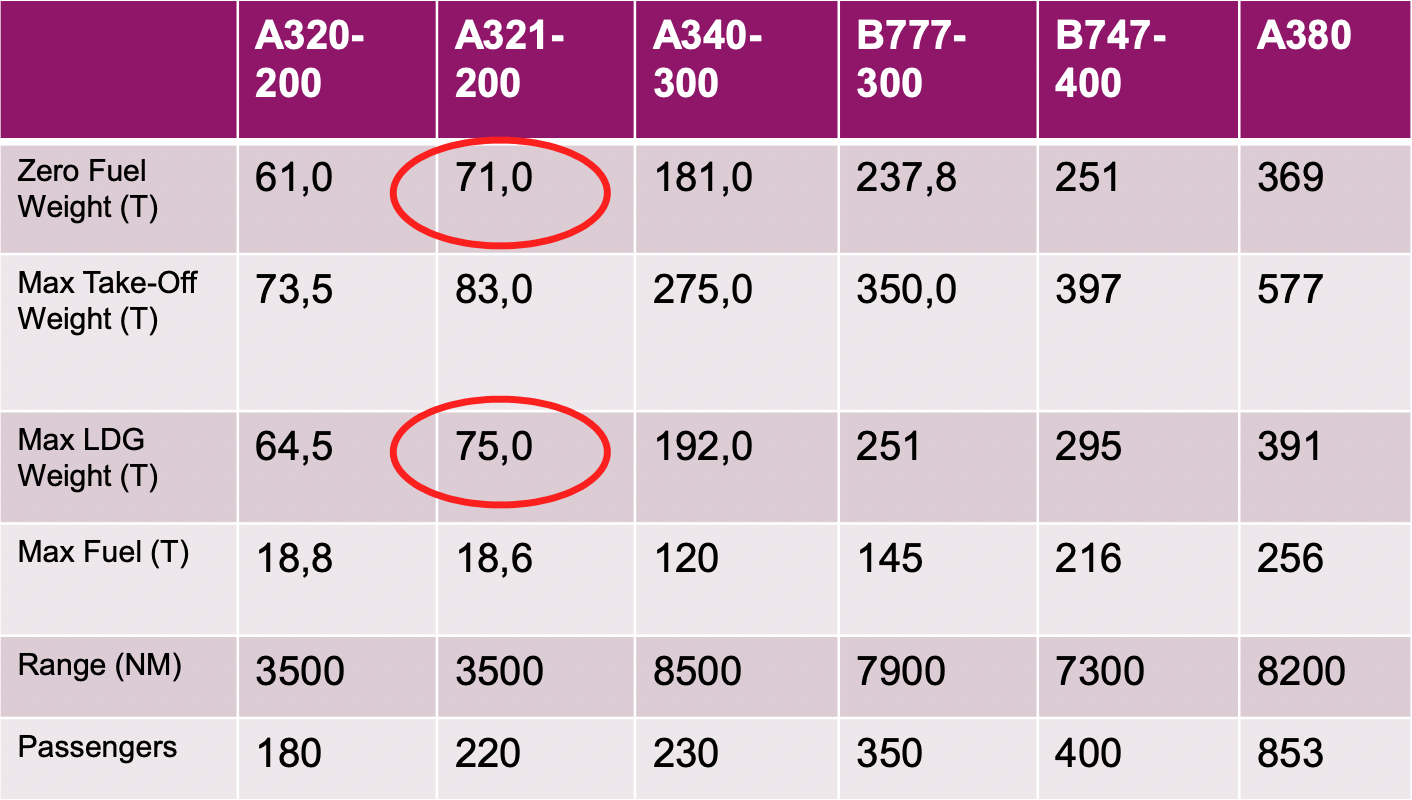
\includegraphics[width=9cm]{Images/Weights.png}
\end{center}
\newpage
\section{Aircraft Operations}
\underline{\textbf{Abbreviations}}
\begin{itemize}
    \item AFIS: Aerodrome Flight Information Service
    \item AFM: Aircraft Flight Manual
    \item ALT: Altimeter
    \item AI: Attitude indicator
    \item ASI: Air Speed Indicator 
    \item FIC: Flight Information Center 
    \item GA or MISAP: Go Around or Missed Approach
    \item IAS: Indicated Air Speed 
    \item KIAS: Knots indicated Air speed 
    \item ROC: Rate of Climb 
    \item RTF: Radiotelephony 
    \item V STALL: Stall Speed
\end{itemize}
\underline{\textbf{Flight Sequence of ZRH-LHR with an A320}}
\begin{enumerate}
    \item Prep at home 
    \item Checkin/ Pre-flight Planning 
    \item At the Gate 
    \item Pushback
    \item Taxi 
    \item Take-Off 
    \item Climb 
    \item Cruise 
    \item Descend 
    \item Approach 
    \item Landing 
    \item Turnaround
\end{enumerate}
\underline{\textbf{1 - Preparation at Home}}
\begin{itemize}
    \item Duty Time (65-90 min before Start of Duty until 30min after official End of Duty)
    \item Block Time (Rolling until Parking, in Duty Time)
    \item Flight Time (Take-Off until Landing, within Block, hence also Duty Time)
    \item Rest Period in Home Base: Matches previous Duty Time or 12hours (the greater one)
    \item Rest Period abroad: Previous Duty Time or 10 hours (the greater one)
    \item Block Times: 100 hours in 28 days or 900h per calendar year 
    \item Duty Times: 13 hours per day (depending on check in times and delays), 60 hours per week (7 days) or 2000h per calendar year
    \item \textbf{Chart} Studies (airports, routes, public addresses (PA), duty times, specifically Passengers (PAX)/freight, weather WX, political situations)
    \item \textbf{Reserve/Standby}: Short haul 1h, Long-haul 1.5h
    \item \textbf{Crew}: Seating Position: CMD Commander and COPI Co-Pilot (1,2), 1 Senior Cabin Member (Maitre de Cabine) \& 3 Cabin Members (on A320)
    \item Commander Rank: Senior Captain, Captain (4 stripes), Co-Pilot: Senior First Officer, First Officer (F/O) or Second Officer (3 Stripes, 2 Stripes)
\end{itemize}
\underline{\textbf{2 - Check-In (T-65')}}
Crew meets, collects documents, planning
\begin{itemize}
    \item Airport: Departure Aerodrome (AD) and Destination AD
    \item Intermediate Alternates: 
    \begin{itemize}
        \item Short haul: Reachable within 60 min at one-engine operative (OEI) cruise speed 
        \item Long haul (3 and 4 engines): 120 min 
        \item ETOPS: Extended Twin Operations (A330): 180min
    \end{itemize}
    \item Flight preparation: Weather: Weather assessment documents 
    \begin{itemize}
        \item General Weather assessment (SWC: Significant Weather Chart)
        \item Satelite Images 
        \item Wind \& Temperature Charts 
        \item Weather Forecast (TAF: Terminal Aerodrome Forecast) - long range forecast (9/18/24 or 30 hours)
        \item Current Weather (METAR: Meteorological Aerodrome Report)
        \item Airports must fulfil certain general minima for sight and/or cloud cover
        \item Report Details Slide 14
    \end{itemize}
    \item Flight preparation: NOTAM (Notice to Airmen): Info for airfields (constructions), airspaces, hazards (radioactive materials)
    \item Flight preparation: Operation Flight Plan (OFP)
    \begin{itemize}
        \item Performance
        \item Mass \& Balance 
        \item Fuel Calculation
        \item Route 
        \item ATC (Air Traffic Control) Flight Plan 
    \end{itemize}
    \item Cabin Briefing: Meet crew and inform them about flight, flight time, PAX, weather (turbulence), stopover
    \item Weights and Fuel (ZFW = A/C + Crew + Freight/PAX):
\end{itemize}
\begin{center}
    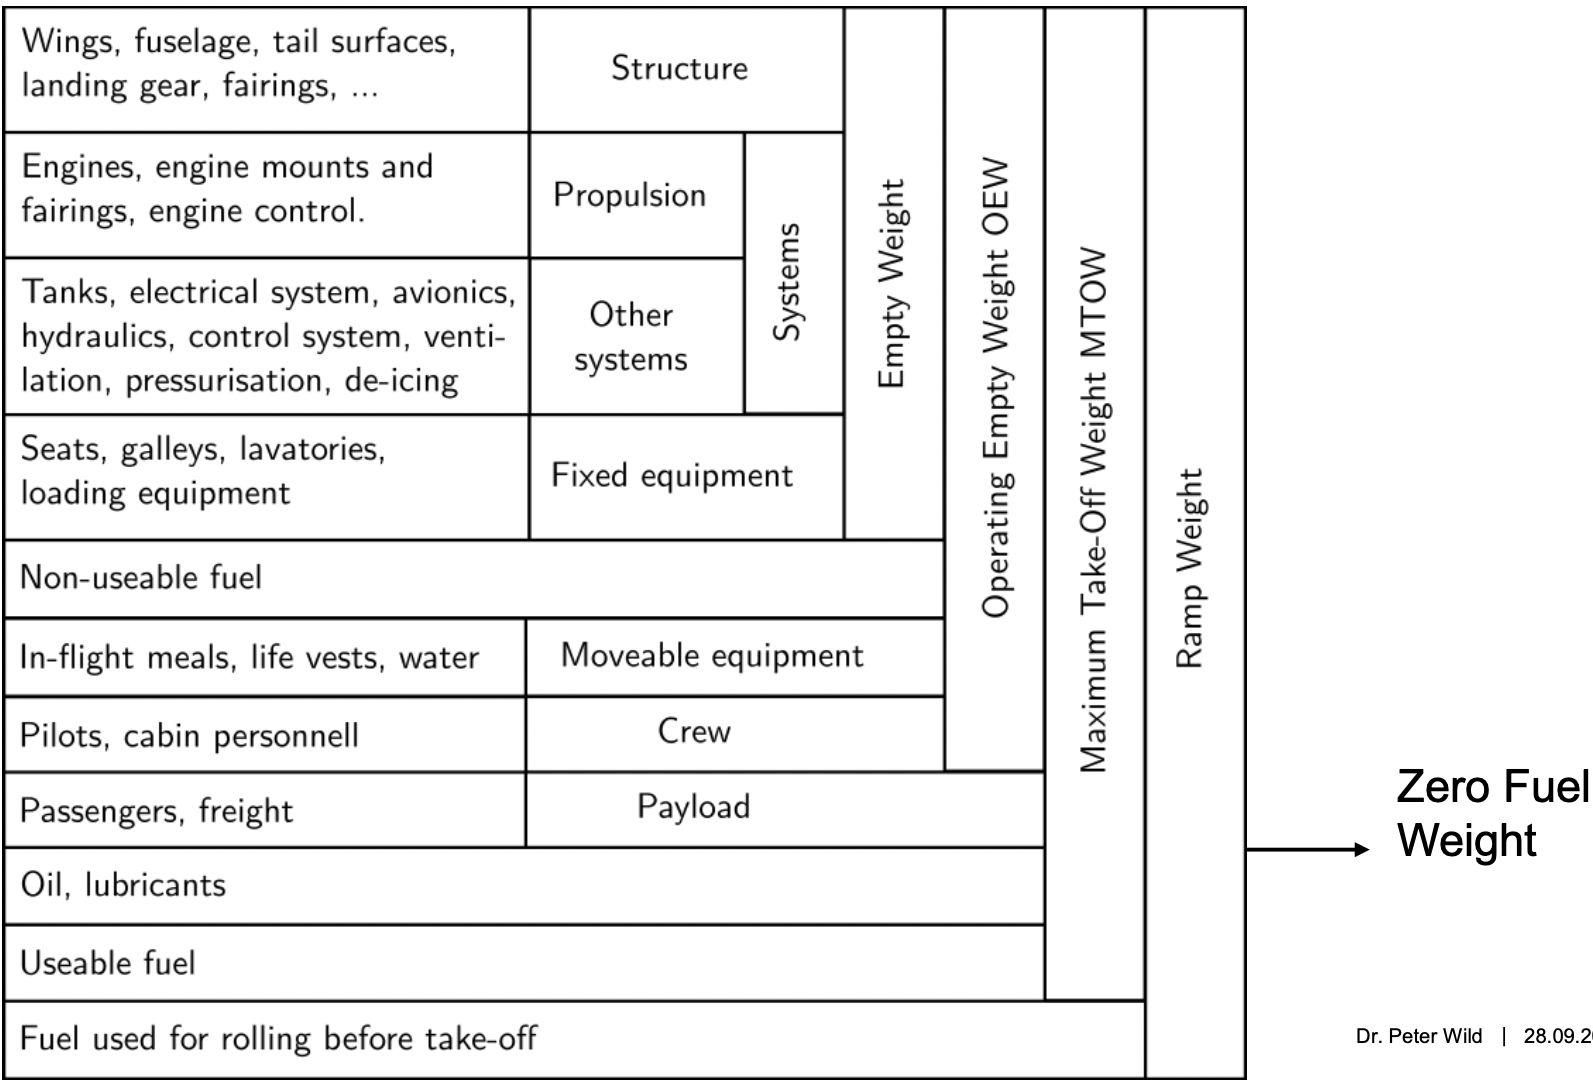
\includegraphics[width=9cm]{Images/Weight_and_Fuel.png}
\end{center}
\begin{itemize}
    \item For different Aircrafts, there is a maximum landing weight (Max LDG/MLDG), which is larger than the zero fuel weight. Weigths above the MLDG will require a checks on the aircraft after landing if they are exceeded. (See slide 21 for details)
    \item (T-40) Bus to Aircraft: Security checks, ID check for Non-Schengen Areas, Own bus 
\end{itemize}
\underline{\textbf{3 - At the Gate/Stand}}
\begin{itemize}
    \item Aircraft: Power through GPU (GNU Power Unit) or APU (Auxiliary). Cooling (air) through Airport or APU.
    \item CMD: Walk around, aircraft acceptance (Aircraft Log/MEL), fuelling
    \item COPI: Cockpit Preparation, FMS (Flight Management System) loading (route \& wind automatic)
    \item Cabin: Safety equipment check (fire extinguisher, axe, gloves, medical kits, cabin search, PBE (protective breathing equipment))
    \item Catering: Load food, drinks, newspapers for booked PAX 
    \item Maintenance: Solve technical problems reported by maintenance / last crew (topping up oil, tyre pressure)
    \item Water/Waste: Empty toilets/refill, fill up water as required
    \item Loading Crew: Load aircraft with ULD (uniform load devices with luggage etc.) 
    \item Overview: See slide 26 (stakeholders)
    \item T-20 (Cabin): Boarding begins: Special PAX first, Unaccompanied Minors (UM), Wheelchairs, Deportees, Medical (Blind, Deaf, Stretcher, Oxygen), Families, Musical Instruments, and anything connected with seating restrictions
    \item Finish Checklists: Cockpit Preparation. Take-off briefings
    \begin{itemize}
        \item Departure Briefing (ATC Clearance) (SID= Standard Instrument Departure) departure route 
        \item Emergency Briefing: Procedure if aircraft experiences and engine failure or any other emergency (fire, both engines damaged)
    \end{itemize}
    \item T-3 (Cabin): Boarding completed (headcount agrees). Coordinator (GND Handling Agent) confirms completion/PAX numbers and brings loading sheet (mass \& balance) as well as NOTOC (Notification to Captain)
    \item NOTOC: Dangerous Good (what kind of), Volume/Weight, Where loaded (ULD NR.), UN Classification, Emergency Response Drill (info Fire Brigade etc.)
    \item (Ground): Complete Loading completed, Pushback tractor gets into position 
    \item T-0 (Cabin): Close doors and arm them (including slides for evacuation)
    \item (Cockpit): Official ATC Clearance obtained for Departure Route \& Pushback. Passengers are greeted over Public Address (PA)
    \item Engines are started during the Push with the help of the APU   
\end{itemize}
\underline{\textbf{5 - Taxiing to Runway }}
\begin{itemize}
    \item The ATC determines the take-off sequence based on traffic and route 
    \item Different checks are made during taxiing 
    \item The cabin crew prepares the cabin (trolley, stowaway items) and shows safety on board film 
    \item \textbf{Influence on Departure and Landing Sequence by categories of Aircraft (WTC: Wake turbulence category)}: 
    \begin{itemize}
        \item J/SUPER (A380)
        \item H/HEAVY (136'000 kg or 3'000'000 LBS) or more
        \item M/MEDIUM (less than H and more than L)
        \item L/LIGHT (7000 kg 15500 LBS) or less
    \end{itemize}
    \item Seperation and LDG: The WTC category defines a separation minimum (in Nautical Miles) from a leading to a following aircraft. Optimally, smaller planes go ahead
    \item Takeoff T/O Minimum (IFR, instrument flight rules): An instrumentally derived horizontal distance a pilot should see down the runway from an approach end, based either on the sighting of high intensity runway lights or on the visual contrasts of objects, whichever yields the greater visual range.
    \item Wind limits and contaminated runways: Crosswinds, tailwinds (normally 10KTS) assumed, and based on runway contamination, different thrust profiles have to be chosen 
\end{itemize}
\underline{\textbf{6 - Take-Off}}
\begin{itemize}
    \item Performance Calculations TORA and ASDA, 2nd Segment (to 400 ft, 2.4\% Gradient), Obstacle Clearance
    \item V1 (if smaller, take-off is rejected), Acceleration to VR (take-off rotation starts), V2 (flight continues with this max speed, climb)
    \item Take-off run acceleration (TORA): Acceleration to V1, then one engine fails with acceleration to VR and rotating 
    \item Accelerate Stop Distance Acceleration (ASDA): Acceleration to V1, then reject and stop on runway 
    \item 2nd Segment: Regulations from Authorities: Gradient 2.4\% with one engine operative (normal OPS 13-27\%) and usually for all engine climbs 3.3-10\%
    \item Obstacle clearance
\end{itemize}
\underline{\textbf{7 - Climb}}
\begin{itemize}
    \item FL (flight level) 100 (depending on pressure, but normally 10'000 ft), altitude at standard air pressure: Max 250 KN 
    \item Over FL 100: Speed determined by airline/manufacturer, for optimum efficiency: Normally 280-320 KTS 
    \item Max FL390 (around 37'000 ft): low weight / valid for most airliners 
    \item FL 390: 27 min / 1900 kg fuel burn / 180 NM speed
\end{itemize}
\underline{\textbf{8 - Cruise}}
\begin{itemize}
    \item Flight Measurement System (FMS) suggest MAX FL, and based on weight and wind + temperature optimum FL 
    \item MACH around 0.78 (depends on outside temperature, but assume normally 300 m/s or 1080 km/h for speed and sound)
    \item Step Climbs: As the aircraft burns fuel, it becomes lighter and climbs to optimum cruise level. In practice, a step climb is carried out  
    \item \textbf{Terrain/Obstacle Clearance}: Maps are published for minimum flight altitude (MGA, grid altitude), minor sector altitude MSA or min Terrain clearance altitude MTCA.
    \item They all guarantee following margins (even though differently calculated)
    \begin{itemize}
        \item Obstacles up to 6000 ft: 1000 ft Margin 
        \item Obstacles above 6000 ft: 2000 ft Margin 
    \end{itemize}
    \item Tasks while cruising: 
    \begin{itemize}
        \item Flying pilot (FP): Flying, navigation, passenger announcements. Pilot monitoring (PM): Radio, Calculations, systems monitoring. Preparation of turnaround (30-40 min on ground): weather, flight planning, fuel, organisation of trouble-free sequence on ground 
        \item Cabin: starts with seatbelts sign off (FL 100) until seatbelts sign on (15 min befor Landing)
    \end{itemize}
    \end{itemize}
\underline{\textbf{9 - Descent}}
\begin{itemize}
    \item Top of Descent (TOD):Flight Monitoring System (FMS) calculates ideal descent taking constraints into consideration. Speed and attitude readings from approach are determined
    \item Calculation: Normally a 3 degree descent or 5.2\%, distance * 3 = nominal height 
    \item Performance: 17 min / 170 kg Fuel / 110 NM 
\end{itemize}
\underline{\textbf{10 - Approach}}
\begin{itemize}
    \item Types of Approaches: Precision Approach, or Non-Precision Approach. Main difference: Non-Precision approach only guides flight crew on lateral axis. Precision approach also on vertical 
    \item Precision Approach: An ILS (instrument landing system) is consists of a localizer (lateral) and a glideslope (vertical). The glideslope leads the aircraft on a 3° angle to the runway. Red/white station and larger beacons
    \item Non-Precision Approach:
    \begin{itemize}
        \item VOR (VHF omnidirectional range): Allows naviagition on a specific course on or away from the station (FR=from and TO=to, multiple stations 1-6, given in degrees, readings agree with map). VOR station is circular
        \item NDB (Non-directional beacon): NDB only shows the route to/from the station. NDB station is a large antenna above ground 
        \item RNAV/GPS (Area navigation/ global positioning system): Aircraft-based platform which can self determine its position wih the help of VOR, ILS, NDB, GPS and IRS (inertial reference system). Independent from ground (satelite based) and support direct routes instead of routes from station to station
    \end{itemize}
    \item Approach type? Depending on:
    \begin{itemize}
        \item Weather: Non-precision approaches need better weather conditions. due to imprecisions. Basically 500ft ceiling (cloud cover), 1500m visibility (ILS: only needs 220ft and 500m)
        \item The on/board aircraft installations 
        \item Qualification of Crew members (for Cat. 2 or 3 approaches)
        \item Needs of the crew (training)
        \item Preference of the airfield/ATC (Noise, efficiency)
    \end{itemize}
    \item Fog - Low visibility approaches:
    \begin{itemize}
        \item Cloud base 200ft/500m visibility: Cat 1 approach via ILS. If visibility is below 400m RVR, then low visibility approach. Lower sequences, greater spacing in the air and on the ground are consequence
        \item Category 2: 100ft/300m. Requirements: Qualified crew, minimum 1 auto-pilot (AP), 2 Pilots, Procedure Autoland
        \item Category 3A: 50ft/200m. Requirements:Additionally to Cat 2, autothrust 
        \item Category 3B: No/75m. Requirements: Additional to Cat 3A, 2 AP, auto rollout and also often auto brake 
    \end{itemize}
\end{itemize}
\underline{\textbf{11 - Landing}}
\begin{itemize}
    \item Begins 50ft on the centerline and should be landed within 300-600m in touchdown zone 
    \item Braking: Carbon brakes, Reverse Thrust, Ground Spoilers 
    \item The landing distance is defined as the effective distance from 50ft above ground until still stand. A safety margin is built in. Measuring the landing distance, this LD=60\% Length of required landing distance needed. Margin is total Runway (TR - LD/0.6 = Margin)
\end{itemize}
\underline{\textbf{12 - Standing at place or at gate + Turnaround}}
\begin{itemize}
    \item Rolling to standing place via signs or marshalls
    \item GPU is attached or APU switched on when engines are shut down
    \item Turnaround time is 30-40 min. This includes
    \begin{itemize}
        \item Passengers leave
        \item Aircraft is cleaned up 
        \item Catering restocked 
        \item Planning completed and A/C refueled 
        \item Checks/safety checks completed 
        \item Boarding starts again
    \end{itemize} 
\end{itemize}
\newpage
\section{Aircraft Aerodynamics}
\begin{itemize}
    \item Lift: Aerodyn. Force perpendicular to the flight vector
    \item Drag: Aeordyn. Force in opposite direction to flight vector
\end{itemize}
\begin{itemize}
    \item Standard condition: $H = 2000 m$ and $\rho = 1~kg/m^3$
\end{itemize}
\underline{\textbf{Fuel consumption}}
\begin{equation*}
    Fuel~burn~per~distance \approx \frac{SFC}{M_\infty} \frac{Weight}{Lift/Drag}
\end{equation*}
$M_\infty$ affected by aerodynamics and Engine, Lift and Drag by Aerodynamics, SFC by engine \\ \\
Equilibrum of forces: Drag=Thrust (minimse thrust), Lift = Weight (mandatory). Design goal Lift $\gg$ Drag \\ \\ Flight Performance: How far: $c_L/c_D$, How long: $c_L^3 / c_D^2$ \\ \\
\underline{\textbf{Forces}}
\begin{align*}
    F_D = c_D \frac{1}{2}\rho_\infty V_\infty^2 A~~/~~F_L = c_L \frac{1}{2}\rho_\infty V_\infty^2 A = mg = L
\end{align*}
The fuel consumption depends on the drag ``Area'': $c_D A$ \\ \\
\underline{\textbf{Eq. of motion}}
\begin{align*}
    &T cos\alpha - D - mg sin\varphi = 0 \\
    &L + T sin\alpha - mg cos \varphi = 0 \\
    &\Theta = Attitude = \alpha + \varphi = AoA + flight/climb~angle  
\end{align*}
\underline{\textbf{Why does a wing generate lift}}: The wing diverts a mass of air downwards. For this the wing acts with a force to the fluid. In return the air generates a force of the same magnitude to the wing (actio = reactio). \\ \\
\underline{\textbf{Induced Drag (Drag due to Lift)}}
\begin{align*}
    D_i &= \frac{2}{\rho V^2 \pi}\left(\frac{L}{b}\right)^2~~,~~F^* = \pi/4 b^2 (Prandtl) \\
    c_{D_i} &= \frac{1}{\pi}c_L^2 \frac{F}{b^2} = \frac{c_L^2}{\pi \Lambda} \\
    b &= Wing~Span, F=Wing~Area, \Lambda = Aspect~Ratio
\end{align*}
\begin{itemize}
    \item Induced drag ($D_i$) depends on ratio of lift and wing span 
    \item The coefficent of induced drag ($c_{D_i}$) depends on the aspect ratio 
    \item A slim wing with high aspect ratio produces less induced drag than a compact wing with small aspect ratio
    \item Induced Drag stems from the principle of linear momentum. No friction is included. The induced drag is an additional contribution to total drag 
    \item In general however, for non elliptical lift distribution, an Oswald-Factor $e$ must be considered $c_{D_{i,true}} = c_{D_{i}} / e$ 
\end{itemize}
\underline{\textbf{Tip Vortices}}
\begin{itemize}
    \item Consider Oswald factor $e$
    \item Heavy Aircraft $\rightarrow$ Strong tip vortex $\rightarrow$ High Separation Distance / Time 
\end{itemize}

\underline{\textbf{Drag}}
Total Drag = Induced Drag + Parasite Drag 
\begin{itemize}
    \item Parasite Drag is depending on the Reynolds, Mach number and some velocity regimes
    \item Influence of Reynolds number: Laminar, turbulent flow and separation. Separation mainly due to pressure drag, turbulent and laminar flow due to friction drag (small contribution)
    \item Target of small drag: No separation, turbulent downstream and large range laminar flow
    \item Incluence of Mach Number: At airspeed M $\geq$ 0.7, the flow is no longer incompressible. Additional drag occurs
    \item Lift and drag depend on the angle of attack. The polar diagram describes the dependence of the lift and drag coefficients on the angle of attack $\alpha$
    \item Following components can lead to drag: skin friction drag, induced drag, profile drag, form drag, compressibility drag, interference drag, base drag, trim drag
\end{itemize}
\underline{\textbf{Flight Performance and characteristics}}
\begin{itemize}
    \item Atmosphere: Aerodynamic Forces depend on the air density. The engine power (thrust) depends on the ambient pressure and temperature
    \item Steady thrust: $tan \varphi = \frac{T cos \alpha - D}{T sin \alpha + L}$
    \item Without thrust: $tan \varphi = \frac{-D}{L} = \frac{-c_D}{c_L} = \frac{height}{distance} $ flight path angle points downwards
    \item $\varphi$ is a measure for the aerodynamic quality of an airplane (how far it can travel from a given altitude)
\end{itemize}
\underline{\textbf{Drag at steady horizontal flight}}
\begin{align*}
    &L = mg = c_L \frac{\rho}{2} V^2 F \\
    &V = \sqrt{\frac{2mg}{\rho F c_L}} \\
    &c_L = \frac{2mg}{\rho V^2 F} \\
    &D = D_{parasite} + D_{ind} = c_{D,para} \cdot \frac{\rho}{2}V^2 F + \frac{\rho}{2} V^2 F \frac{c_L^2}{\pi \Lambda e} \\
    &= \frac{\rho}{2} V^2 F (c_{D,para} + c_{D,ind}) = K_1 V^2 + K_2 \frac{1}{V^2}
\end{align*}
The function $D(V)$ intersects with the function of Thrust $T(V)$ twice due to its shape. There are two optimal points with velocities $V_1$ and $V_2$, where there is no excess thrust or drag ($T=D$). However the stall speed is determined as follows with the maximal Lift coefficient from the polar diagram:
\begin{equation*}
    V_{stall} = \sqrt{\frac{2mg}{\rho F c_{L,max}}}~~~(c_{L,max} = c_{a,max} ~from~diagram)
\end{equation*}
\begin{itemize}
    \item The maximum speed (ideally $V_2$ is determined from the maximum Thrust ($V_max, horiz$))
    \item The minimum speed is the stall speed $V_{stall} > V_1$
    \item The speed range is between minimum and maximum speed
\end{itemize}
\underline{\textbf{Stability control}}
\begin{itemize}
    \item Steady flight condition $\rightarrow$ Disturbance $\rightarrow$ Answer of airplane $\rightarrow$ Flight path
    \item Example: Horizontal flight, then Pilot command: elevator deflection or gust comes, then pitching moment, then determine if stable/unstable/indifferent
    \item $alpha$, $\Delta \alpha > 0$, $-\Delta c_m$, $\frac{dc_M}{d\alpha} > 0$ (positive criterion)
    \item Lilienthal: Positive long. stability, Wright: Negative long. stability
    \item Dassault Falcon: stable, Neuron (delta wing): instable, Raffale: indifferent/neutral
\end{itemize}
\underline{\textbf{Development trends}} \\ \\
Good airplane
\begin{itemize}
    \item High lift to drag ratio (low drag)
    \item High ratio of payload to weight (low empty weight)
    \item High engine efficiency (high ratio of engine diameter to shaft power for propeller) + high compressor, combustor and turbine efficiency
\end{itemize}
Highest efficiency drivers
\begin{itemize}
    \item Engine: -15\% (high combustion efficiency, geared fan)
    \item Energy: -5 \% (no bleed air, more electric aircraft)
    \item Aerodynamics: -10 \% (Wing tip, engine integration, empennage config, Detail improvement)
    \item Structure: -5\% (Detail improvment, composites, new alloys, new joining technologies)
    \item Air traffic management
    \item New configurations revolutions vs. tube-wing evolution (curent)
    \item Electric/hybrid aircraft - new design freedom
\end{itemize}
\newpage
\section{Manufacturing and Maintenance}
\underline{\textbf{Abbreviations}}:
\begin{itemize}
    \item A/C: Aircraft
    \item AMM: Aircraft Maintanance Manuals (Detailed instructions)
    \item AMP: Aircraft Maintenance Program
    \item CAMO: Continuing Airworthiness Management Organisation
    \item CRS: Certificate of Release to Service
    \item DIS: Discard
    \item DOA: Design Organisation Approval
    \item EASA: European Aviation Safety Agency
    \item ETOPS: Extended Range Twin Operations
    \item FAA: Federal Aviation Agency
    \item FC: Flight Cycles
    \item FH: Flight Hours
    \item FNC: Functional Check 
    \item IFE: In-flight entertainment
    \item MEL: Minimum Equipment List 
    \item MOE: Maintenance Organisation Equipment
    \item MSN: Manufacturer Serial Number 
    \item MX PFC: Maintenance Pre Flight Check
    \item OPS: Operational Check  
    \item PFC: Pre Flight Check
    \item POA: Production Organistion Approval 
    \item RST: Restore (Overhaul)
    \item SPC: Special Check 
    \item STC: Supplemental Type-Certificate 
    \item TC: Type Certificate 
    \item XWB: Extra Wide Body
\end{itemize}
\underline{\textbf{Manufacturing - Initial Airworthiness}} \\ \\
\underline{\textbf{A350 XWB Program Summary - see slides 7-9 }} \\ \\
\underline{\textbf{Tasks in Approval of the A350 XWB}}
\begin{itemize}
    \item MSN1: Initial Handling, Systems \& Powerplant Tangentensteigung
    \item MSN2: Cabin Certification, early long-flight tests, in-flight entertainment (IFE), cabin hot \& cold testing, visit the McKinley Climatic Lab in Florida, USA
    \item MSN3: High altitude (Bolivia) and cold weather (in Canada) testing, performance and measurement, hot and cold weather campaigns, systems and powerplant testing 
    \item MSN4: External Noise, and lightning tests, avionics development/certification, training for pilot and maintenance 
    \item MSN5: Cabin operability training, route-proving, ETOPS (extended twin operations) certification
\end{itemize}
Comparing A350 to A340 Final Assembly: A 350 has at first the fuselage completed, then the wings are attached. For the A340, the center fuselage with the wings are first assembled. \\ \\
Important information:
\begin{itemize}
    \item A350 XWB uses mostly Carbon Fiber Reinforced Polymer (53\% weight)
    \item An Iron Bird is a zero-test rig, which is used to test hydraulic, electrical and flight control systems. It has the same components as installed on MSN1. It is also used to test the interface between Cockpit and A/C systems
    \item The McKinley Climatic Lab is used to demonstrate the whole operational spectrum of the aircraft on ground 
    \item The EASA is the primary certification authority for A350, whereas the FAA is the primary cert. auth. of Boeing A/C. The FAA or EASA validates the approvals of their respective counterparts (bilateral agreement US-EU)
    \item Multiple screens of same type are used in the cockpit - why? Dispatch reliability/exchange capability, less stock of screens required by operator
    \item The A350 has an ETOPS Approval of 370min (2500 NM)
    \item Common Type Rating: Is approved by EASA as a way for decreasing the time of training required by a pilot to change from an  A330 to an A350. Cross Crew Qualification normally takes longer (slide 15 details)
\end{itemize}
\underline{\textbf{Regulatory Basics for Certification in Europe - Airworthiness}}
\begin{itemize}
    \item Initial Airworthiness (EASA Part 21 + 26 [for passenger A/C], 748/2021 + 2015/640): 
    \begin{itemize}
        \item Airworthiness and environmental certification of A/C and related products, parts and appliances
        \item Certification of Design Organisations (DOA) (Section J)
        \item Certification of Production Organisations (POA) (Section G)
    \end{itemize}
    \item Certification Specifications (CS) for Products:
    \begin{itemize}
        \item CS25: Large Aeroplanes (1100 pages), CS-22: Sailplanes, CS23: Normal, Utility and commuter aeroplanes, CS-27: Small rotorcraft (up to 3.175 tonnes and 9 PAX), CS-29 Large rotorcraft ($>$3.175 tonnes), CS-31 Balloons
        \item CS-34: Aircraft Engine Emmissions and Fuel Venting
        \item CS-36 Aircraft Noise 
        \item CS-E Engines (only engine)
        \item CS-26: Additional Airworthiness specifications for operation (Part 26) - for crew and transport important!
        \item (CS-LSA): Light Sport Aeroplanes, (CS-ETSO): European Technical Standard Order 
    \end{itemize}
\end{itemize}
Examples
\begin{itemize}
    \item CS25.581: Lightning Protection $\rightarrow$ Non-metallic and non-metallic, as mostly today many CFRP wings etc. $\rightarrow$ Static Wicks (Lightning Rods) burn away, in metal planes farrady cage. As well metallic meshes underneath the wing surface
    \item CS25.803: Emergency Evacuation: More than 44 passengers, maximum seat capacity can be evacuated from aeroplane to ground within 90 seconds. Compliance shown by actual demonstration outlined in CS25 Appendix J. 
\end{itemize}
\underline{\textbf{Part-21 Production Organisations in CH (slide 25)}}
\begin{itemize}
    \item 19 in CH, Pilatus, Bucher, Lantal, RUAG Int. (CH.21G.0002,0015,0012,0021)
\end{itemize}
\underline{\textbf{Largest Aircraft Manufacturers}}
\begin{itemize}
    \item Commercial: Airbus, Boeing, (Bombardier), Embraer
    \item Private Large A/C: Bombardier, Cessna, Dassault, Embraer, Gulfstream
    \item General Aviation: Textron Aviation (Cessna, Hawker, Beech), Diamond, Pilatus
    \item Numbers:
    \begin{itemize}
        \item Most produced A/C: Cessna C172 $>$ 44'000
        \item Most produced Heli: Mil Mi-8 $>$ 18'000
        \item Most produced commercial airliner: Douglac DC-03: 16'079 
        \item Largest manufacturere by produced A/C: Cessna $>$ 450'000 A/C since 1945
    \end{itemize}
\end{itemize}
\underline{\textbf{MMEL - Master Minimum Equipment List}}
\begin{itemize}
    \item An A/C is certified with all equipment operative. However defects occur, and the operator wants to fly 
    \item Conditional Deviations from Type Certificate (TC) are authorised $\rightarrow$ Dispatch Conditions 
    \item The Dispatch Conditions are listed in the MMEL 
    \item The MMEL is an approved deviation from the Type Certicficate
    \item MMEL assures an acceptable level of safety while an aircraft is operative with inoperative equipment
\end{itemize}
\underline{\textbf{MEL - Minimum Equipment List}}
\begin{itemize}
    \item The MEL is based on the MMEL
    \item Is developed by Operator, and is less restrictive than the MMEL
    \item Contains operations specific items based on A/C configuration, equipment installed and routes flown (additional requirements on cleaning etc.)
    \item The MEL must be approved by the authority of the operator 
\end{itemize}
\underline{\textbf{Layout of MEL and MMEL}}
\begin{enumerate}
    \item System and Sequence Numbers (Item Reference and designation (ATA breakdown designation))
    \item Rectification Interval (B,C,D may be extended one time)
    \begin{itemize}
        \item A: No standard rect. Interval
        \item B: 3 consecutive calendar days 
        \item C: 10 cons. cal. days 
        \item D: 120 cons. cal. days
    \end{itemize}
    \item Number installed 
    \item Number required for Dispatch (dispatch conditions can be different for different numbers)
    \item Remarks or exceptions (marked through (o), (*) or (m))
\end{enumerate}
\underline{\textbf{Continuing Airworthiness - EASA Part-M, -CAMO, -145 etc.}}
\begin{itemize}
    \item EU No 1321/2014 regulates the continuing of Airworthiness of A/C and aeronautical products, parts and appliances, rights and obligations for organisations seeking approval to carry out following activities:
    \begin{itemize}
        \item Planning for Continuing Airworthiness of A/C is done in the Part-CAMO Organisation (Annex Vc), according to tasks as described in Part-M (Annex I)
        \item Execution of maintenance is done in Part-145 (Annex II) or Part-CAO Organisation (Annex Vd)
    \end{itemize}
    \item EASA Continuing Airworthiness also regulates Part-66 licenses for maintenance personell performing maintenance activities (Annex III)
    \item Rights and Obligations for Part-147 organisations seeking approval to conduct training and examination of Part-66 
    \item Additional requirements for continuing airworthiness of leased-in country aircraft (CAT) (Part-T) Annex Va
\end{itemize}
\underline{\textbf{Planning and Continuing Airworthiness}}
\begin{itemize}
    \item Part-CAMO: Commercial or Complex A/C, there continuing airworthiness is ensured by a CAMO 
    \item Example: Swiss, Helvetic, Pilatus, Rega, Air Zermatt, Jet Aviation Business Jets 
    \item Tasks are described in Part-M
    \begin{itemize}
        \item Creating and updating maintenance program 
        \item Preparing workorders for the required maintenance on the A/C for the respective Maintenance Organisation 
        \item Implementation of all relevant airworthiness directives (AD)
        \item Ensure that maintenance is carried out by an approved organisation
    \end{itemize}
\end{itemize}
\underline{\textbf{Perfomance of Maintenance in a Part-145 organisation}}
\begin{itemize}
    \item Example: SR Technics, Swiss, RUAG, Rega, Pilatus Jet Aviation, Bucher Leichtbau (Maintance organisation)
    \item Is required to provide a suitable facility
    \item Must hav the licensed Part 66 certified personell available
    \item Must have the approval for the type of aircraft and scope (line/light or base maintenance)
    \item Must have necessary equipment, tools and materials 
    \item Must have a QC-System in place
    \item Must have a maintenance organisation exposition (MOE) - org-chart 
    \item Performs maintenance in accordance with the workorder received from the owner or CAMO 
    \item Must record all its work in maintenance records 
    \item Certifies the work performed in the technical logbook on the \textbf{Certificate of Release (CRS)}, which is copied after completion of work (one in aircraft, one on ground, going to CAMO)
\end{itemize}
\underline{\textbf{Licensed Personnel according to Part-66}}
\begin{itemize}
    \item Example: Technician of Aircraft 
    \item Must demonstrate basic knowledge 
    \item Must attend different module-courses and pass exams (license categories)
    \item Training time approx. 2 years 
    \item Must have attended relevant A/C type trainings
    \item Prove experience, as license must be renewed by component authority every 5 years  
\end{itemize}
\underline{\textbf{Part-147 Training organisation}}
\begin{itemize}
    \item Example: SR Technics, Pilatus, Aviotrace, QCM 
    \item Must provide appropriate facilities 
    \item Have apropriate staff 
    \item Must provide teaching material including access to workshops for practical training 
    \item Quality System 
    \item Records of performed courses 
    \item Must have a Maintenance Training Organisation Exposition 
\end{itemize}
\underline{\textbf{Aircraft Maintenance Program (AMP)}}
\begin{itemize}
    \item All maintenance on an aircraft is based on its individual maintenance program 
    \item It must be developed by the operator, bosed on the Maintenance Plannign Document (MPD)
    \item MPD is part of the certification process 
    \item Operator/CAMO can add items or decrease mainteance intervals based on experience made during maintenance
    \item Increase of mainteance intervals is possible in cooperation with the TC holder 
    \item Maintenace intervals (since ops start)
    \begin{itemize}
        \item Line Maintenance:
        \begin{itemize}
            \item MXPFC + PFC: Before each departure 
            \item W (Weekly): All 14 calendar days 
            \item A: Every 800 FH (approx 3 weeks)
        \end{itemize}
        \item Base Maintance
        \begin{itemize}
            \item C: 1C,2C,4C,8C = 18/36/72/144 months 
            \item IV: 1IV = 6Y = 72 months 
            \item D: 1D = 12Y = 144 months
        \end{itemize}
    \end{itemize}
\end{itemize}
\begin{center}
    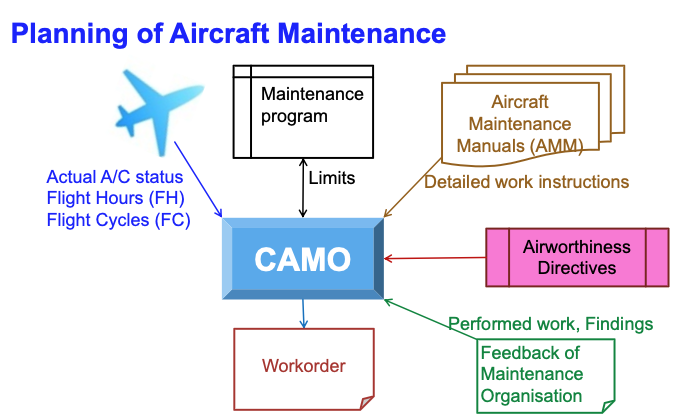
\includegraphics[width=9cm]{Images/Planning of Aircraft Maintenance.png}
    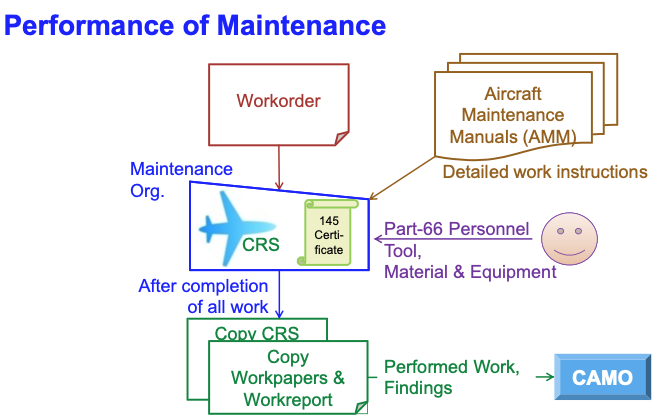
\includegraphics[width=9cm]{Images/Performance of Maintenance.png}
    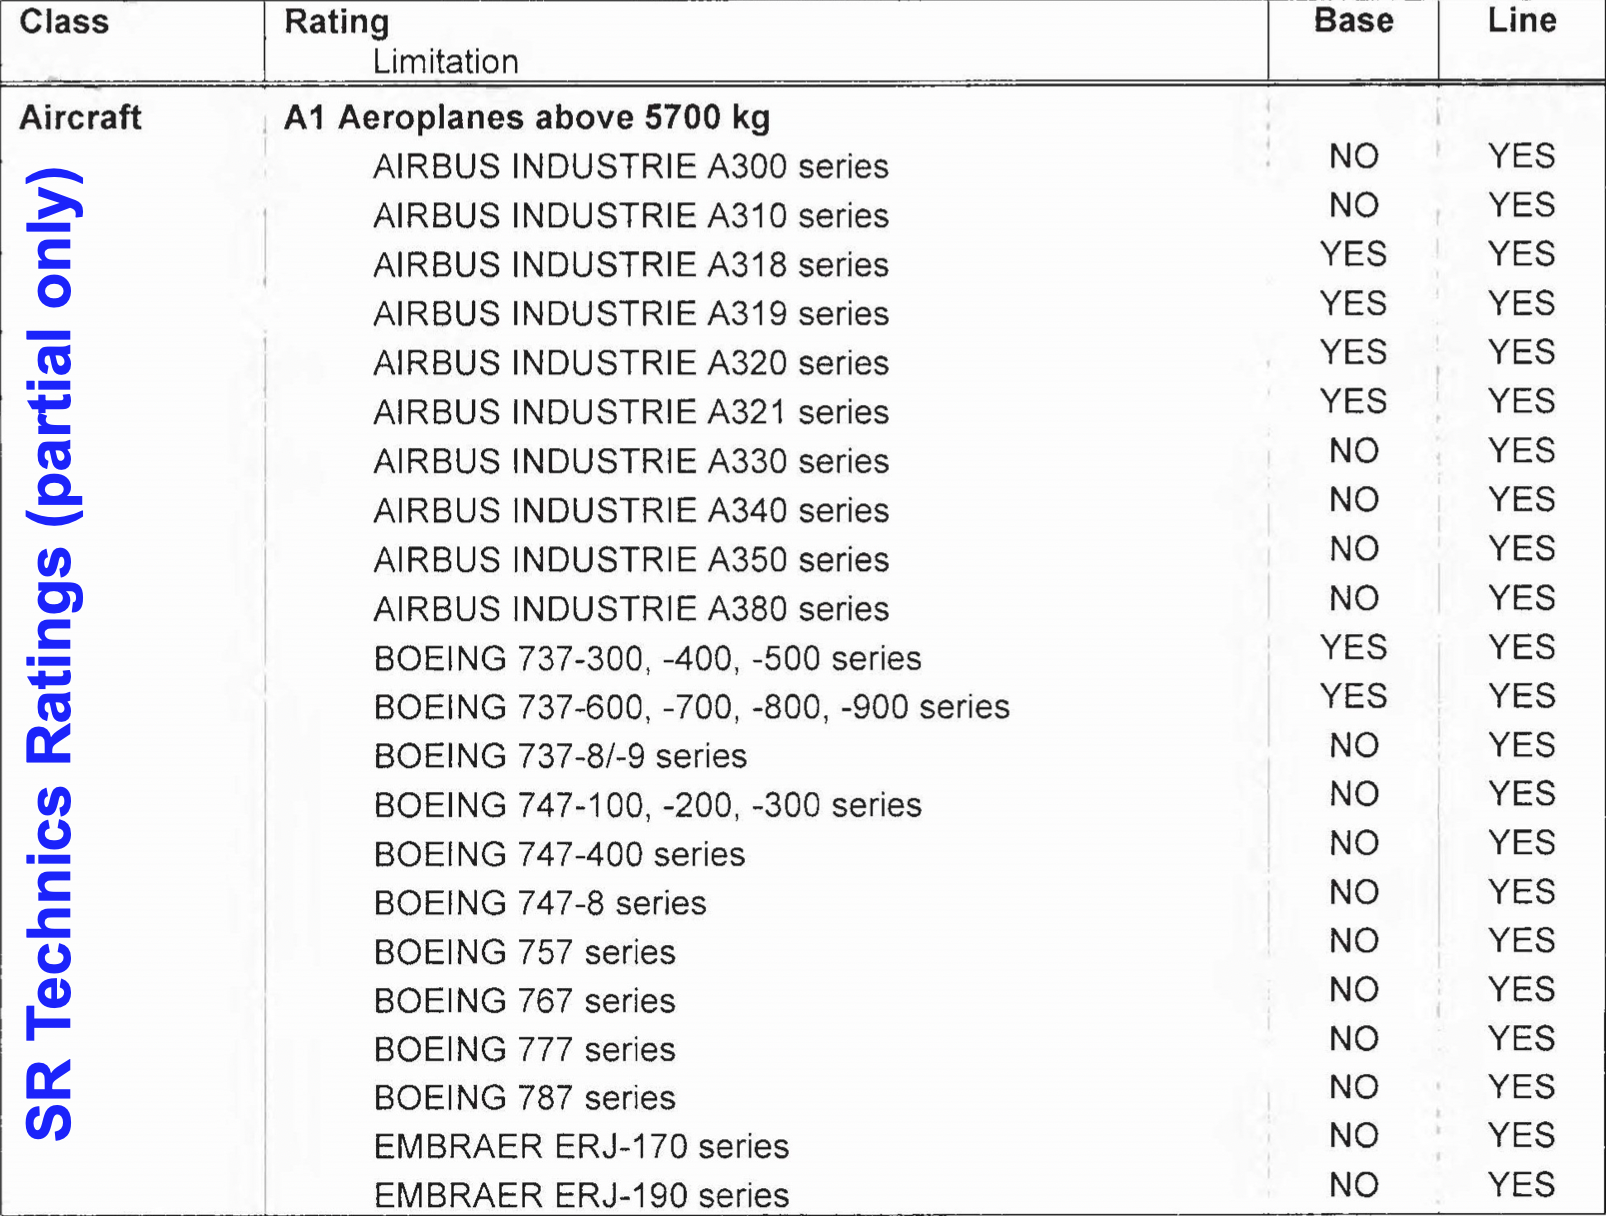
\includegraphics[width=9cm]{Images/Maintenance Rating.png}
\end{center}
\newpage
\section{Military Aviation}
\underline{\textbf{Tasks and capabilities of the Swiss Air Force}}
\begin{itemize}
    \item During times in peace: Surveillance of the airspace + air policing (AP)
    \item During times of peace, crisis and war: Gathering and distribution of intelligence, air transport (heli), and protection of the airspace (air policing, air defense)
    \item In the past: Enemy was known 
    \item Today: Assumption about capabilities and devices of potential adversary
\end{itemize}
\underline{\textbf{Task of the air force}}
\begin{center}
    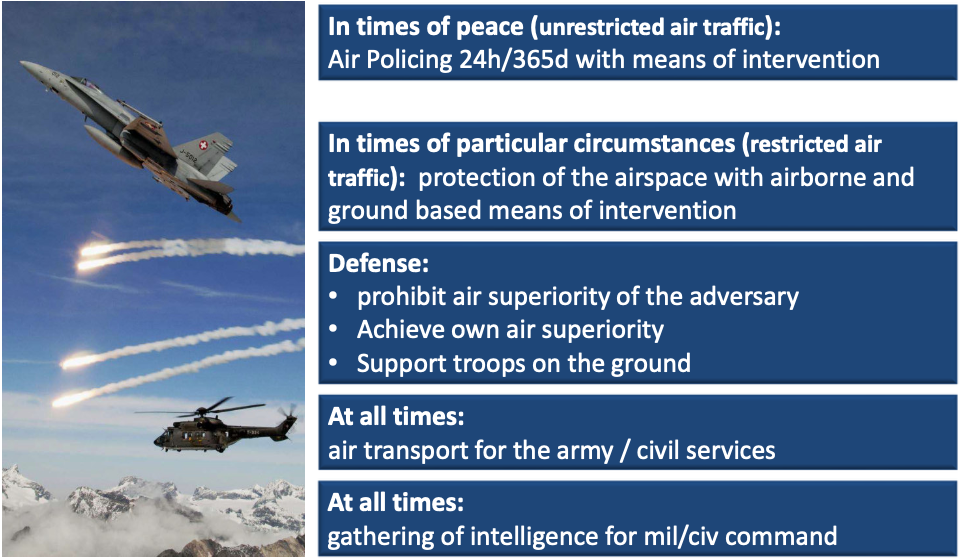
\includegraphics[width=9cm]{Images/Tasks of the air force.png}
\end{center}
\underline{\textbf{Capabilities of the Swiss Air Force}}
\begin{center}
    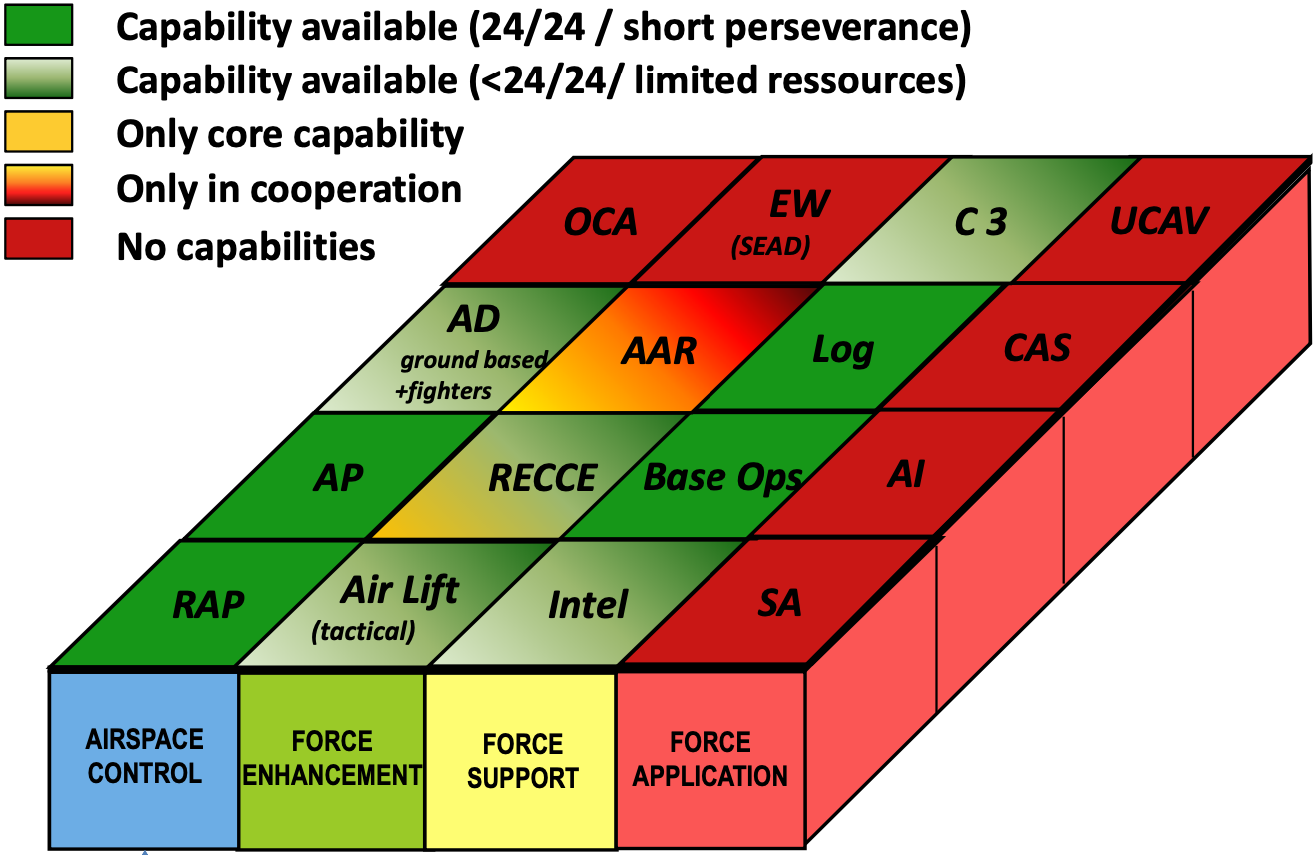
\includegraphics[width=9cm]{Images/Capabilities of the Swiss Air Force.png}
\end{center} 
Abbreviations
\begin{itemize}
    \item RAP: Recognised Air Picture
    \item AP: Air Policing / Air Police
    \item AD: Air Defence 
    \item OCA: Offensive Counter Air 
    \item Air Lift: Air Transport 
    \item RECCE: Aerial Reconnaissance
    \item AAR: Air-to-Air Refuelling
    \item EW: Electronic Warfare 
    \item Intel: Intelligence 
    \item Base Ops: Air Base Operations 
    \item Log: Logistics 
    \item C3: Command - Control - Communication 
    \item SA: Strategic Attack 
    \item AI: Air Interdiction 
    \item CAS: Close Air Support 
    \item UCAV: Unmanned Combat Aerial Vehicle
\end{itemize}
\underline{\textbf{Air Police}}
\begin{itemize}
    \item Identification: of foreign state craft (1/day)
    \item Detection: of airspace infringements (1/week)
    \item Help: In case of problems with navigation or radio communication (1/month). If a transponder is turned off, then the air traffic control (secondary radar) cannot detect airborne vehicle anymore. The military ATC can however detect Position, Altitude, Direction or Speed via a primary radar (+IFF) for RAP
    \item Enforcement: of airspace restrictions (1/year). Two airplanes, one behind and one next to cockpit 
\end{itemize}
\underline{\textbf{Rules when intercepted}}
\begin{itemize}
    \item Intercepting Aircraft: Rocking of weeks = follow me (acknoledged by rocking wings)
    \item Intercepting Aircraft: Abrupt break away = you may proceed (acknoledged by rocking wings)
    \item Intercepting Aircraft: Circles aerodrome and lowers landing gear = land here (acknoledged by lowering landing gear)
    \item Intercepted Aircraft: Gear retraction and irregular switching of all available lights = cannot comply 
    \item Intercepted Aircraft: Flashing of lights = in distress
\end{itemize}
\underline{Enforcement of airspace restrictions}:
\begin{itemize}
    \item 30 F/A 18
    \item Radar, Datalink
    \item Mach 1.6
    \item 20mm  M61A1 Gatling Gun (6000 rpm)
    \item Raytheon AIM-9X Sidewinder (Multipurpose Missile)
    \item Raytheon AIM-120B AMRAAM (Medium Range Air-to-Air Missile)
    \item Helmet Visor 
    \item NVG (Night Vision Goggles)
\end{itemize}
\underline{\textbf{Why WEF requires Constant Air Police}}:
\begin{itemize}
    \item Air fields in Payerne, Emmen and Meiringen are each 10, 7.5 or 5 min away from Davos  
\end{itemize}
Decision making 
\begin{center}
    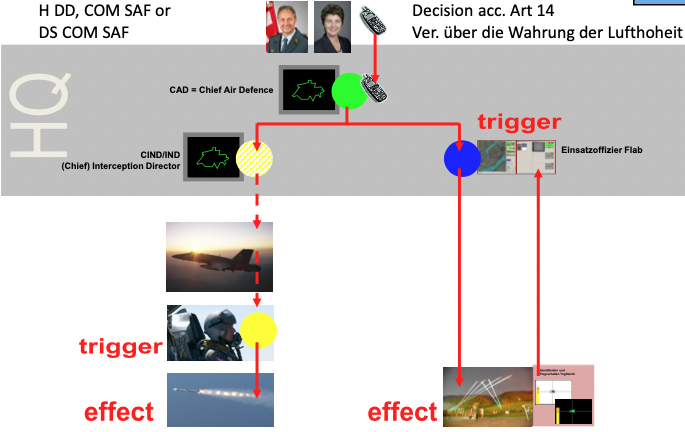
\includegraphics[width=9cm]{Images/Decision_Making_CH_Army.png}
\end{center}
\underline{\textbf{Airspace Control in Times of Peace}}
\begin{itemize}
    \item In unrestricted airspace no weapons may be used against civil air traffic 
    \item In restricted airspace the Head of the Defense Department may order the use of weapons in isolated cases. But only if air policing orders are disobeyed and no other means are available.
    \item The use of weapons is allowed for self defense and helping others in self defense.
    \item Against foreign state air traffic, namely military air traffic, weapons may be used if they enter Swiss airspace without permission or by deliberate deviation from permissions or restrictions and if air policing orders are disobeyed and no other means are available.
    \item International cooperation is not compatible with neutrality.
\end{itemize}
\underline{\textbf{Planning Air Defense and Police}}
\begin{itemize}
    \item 4 fighters (SOP) 144h/d
    \item 3-4 fighters for permanent protection
    \item Readiness 50-70\%
    \item 20 fighters: 100/fighter per 14 days 
    \item Today: 30 F/A 18 each: Can only be used 100h in 6 months 
    \item Pilots: 32 pilots, each 12h/day
    \item Today: 3 Squaddrons, each 16=48 pilots 
\end{itemize}
\underline{\textbf{Airspace Control in Times of Peace, Crisis and War}}
Permanent surveillance of the airspace
\begin{itemize}
    \item In times of restricted air traffic with 4 fighters at all times in the air. Within 3 weeks, already we cannot preserve the AP/AD
\end{itemize}
Quick Reaction Alert (QRA) yesterday and today
\begin{itemize}
    \item Core capacity: Formation and training of our militia component 
    \item Readiness / adapted readiness: Notice at least 24h in advance 
    \item Since 2021: Permanent Air Surveillance: 356d/24h
\end{itemize}
\underline{\textbf{Definitions}}
\begin{itemize}
    \item \textbf{Air Superiority}: That degree of dominance in the air battle of one force over another that permits the conduct of operations by the former and its related land, sea, and air forces at a given time and place without prohibitive interference by the opposing force.
    \item \textbf{Air Supremacy}: A position in war where one side holds complete control of air warfare and air power over opposing forces. It is defined by NATO and the United States Department of Defense as "the degree of air superiority wherein the opposing air force is incapable of effective interference”.
\end{itemize}
\begin{center}
    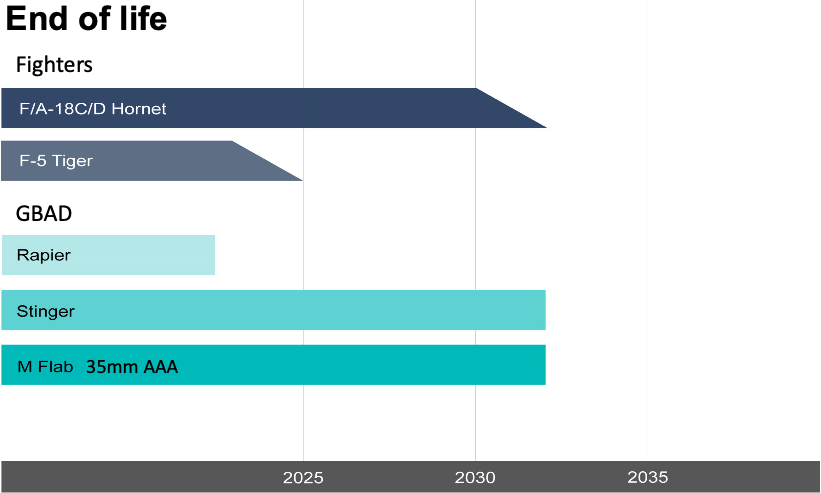
\includegraphics[width=9cm]{Images/End_of_Life.png}
\end{center}
\underline{\textbf{Effects of Gaps in Capabilities for Switzerland}}
\begin{itemize}
    \item Safety of civil air traffic at risk
    \item No protection of endangered civil infrastructure
    \item Limited air defense capabilities
    \item Overall limited defense capabilities
    \begin{itemize}
        \item Useless investment in armored mobility due to air threats
        \item Poor intelligence due to lack of aerial reconnaissance
        \item Increased pressure on our forces due to lack of air to ground capabilities
        \item Poor mobility in impassable terrain near a frontline due to lack of armed air transport
    \end{itemize}
\end{itemize}
\underline{\textbf{Air Lift Mission}}
\begin{itemize}
    \item Transport of troops and material
    \item Emergency relief
    \item Fire fighting
    \item VIP Transport
    \item Dropping of Paratroopers
\end{itemize}
\underline{\textbf{Current Air Transport Missions}}
\begin{itemize}
    \item Transport of troops and materials
    \item For special forces: Infiltration and Exfiltration (low, night)
    \item CASEVAC (Casualty Evacuation)
    \item Peace support operations in Kosovo: readiness to bring international troops to uprisings / riots as fast as possible.
    (+ in Bosnia 2005-2009)
    \item Emergency relief, Fire fighting
    (Albania 99, Avalanches 99, Floods 00, Fires 03, Floods 05, Fires 07 Greece, Fires 10 Israel, drought 15, Fires 16, Fires 17 CH + Portugal + Montenegro + Italy, Floods 17, drought 18, Fire Fighting 18, Greece 21, ...)
    \item VIP Transport
    \item Dropping of paratroopers
\end{itemize}
\underline{\textbf{Helicopters}}
\begin{center}
    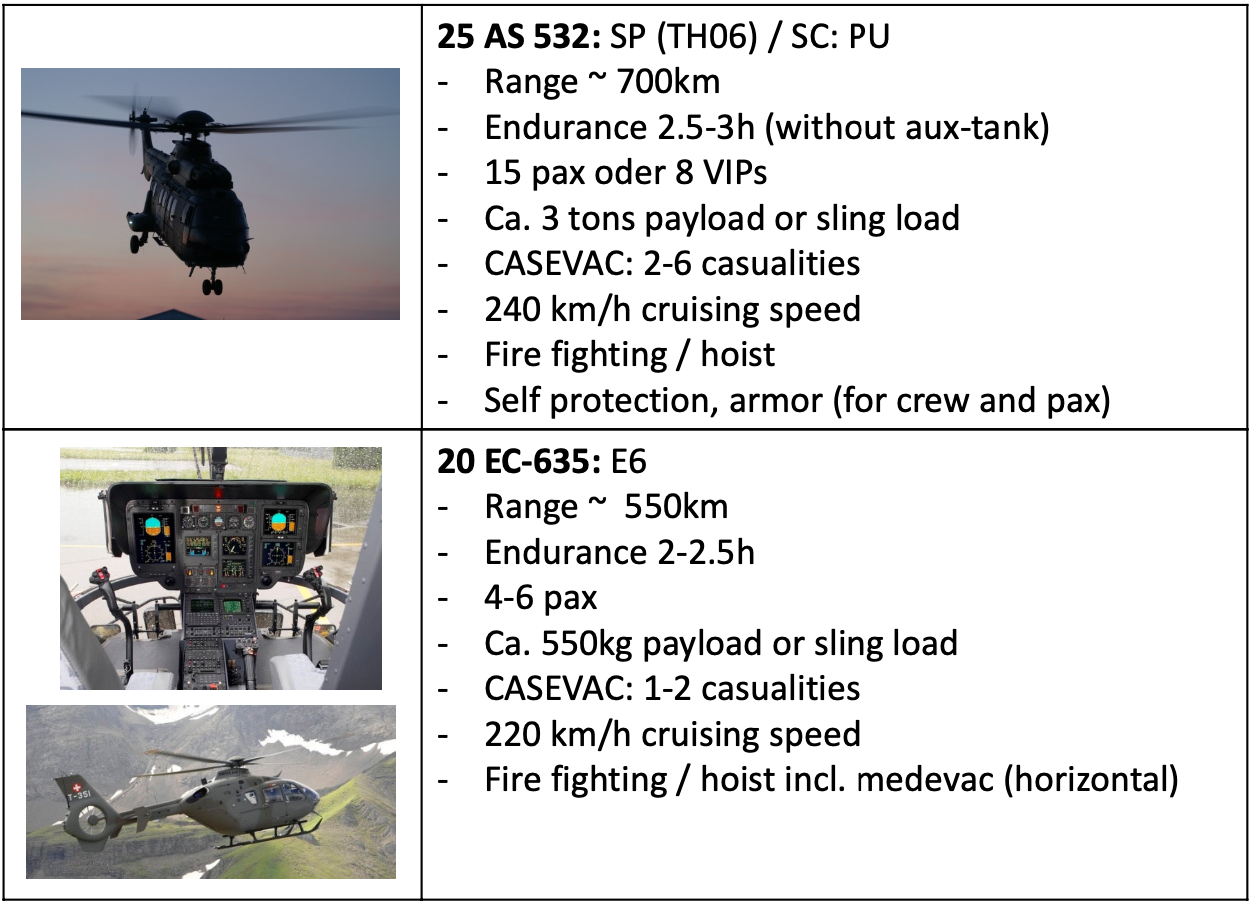
\includegraphics[width=9cm]{Images/Helicopters.png}
\end{center}
\underline{\textbf{Conditions for Helicopter Operations}}
\begin{itemize}
    \item Weather (feasibility, reachibility, IFR: Point in Space Approach)
    \item Distance to mission (slow)
    \item Landing site (~45m Appr, 3m to obstacles, level for landing, demined)
    \item Fuel (Refueling needs time (30' PU, 15' E6, Hotrefuel PU (15'): fire brigade))
    \item Deployed Means (Helicopter, crew) (size, numbers)
    \item Air traffic coordination 
    \item Overnight helicopter, crew (perseverance, comsec)
    \item Maintenance (shelter, logistics)
    \item Flight duty regulations, NVG: whole crew 
    \item Changes of configurations: 30min (sling load) - 1h(Casevac) - 8h (FLIR) - requires time
\end{itemize}
\underline{\textbf{Transport of Troops and Materials}}
\begin{itemize}
    \item It is necessary to be able to evacuate dispersed or entrapped troops or casualties by means of air transport.
    \item This ability is very limited due to the lack of armed air transport
    \item $\rightarrow$ Poor mobility in impassable terrain near a frontline 
\end{itemize}
\underline{\textbf{Means of Aerial Reconnaissance}}
\begin{itemize}
    \item Actual Means 
    \begin{itemize}
        \item 2 Super Puma with FLIR: search for missing persons and missing aircraft
        \item Paratroopers: gathering of information behind enemy lines
    \end{itemize}
    \item Soon:
    \begin{itemize}
        \item Unarmed reconnaissance drone Hermes 900 HFE (Elbit Systems from Israel), inclusive: sensors, ground components, logistics, training, teachingmaterial, ..., for: gathering of information for civil and military commanders: ground troops, police, border control
    \end{itemize}
\end{itemize}
\underline{\textbf{Recconaissance (RECCE)}}
\begin{itemize}
    \item Gap: Fighters with reconnaissance pod or built in abilities
\end{itemize}
\newpage
\section{Air Law}
\underline{\textbf{Licenses}}
\begin{itemize}
    \item Light Aircraft Pilot License (LAPL): Single-engine, land aircraft with piston engine up to 2000kg departure weight, max. 3 passengers/non-commercial (fixed wing A/C, helis, gliders, balloons)
    \item Private Pilot License (PPL): Non-commercial (fixed wing A/C, helis, gliders, balloons)
    \item Commercial Pilot License (CPL): Commercial for certain type ratings (Single Pilot); or classes (for fixed-wing aircraft, helicopters and balloons)
    \item Airline Transport License (ATPL): Commercial/for MPA (multi pilot aeroplane) compulsory (for fixed-wing aircraft and helis)
\end{itemize}
\underline{\textbf{Medical - Validity depends on age} - Slide 9} \\ \\
\underline{\textbf{Class Ratings}}
For aircraft with single-pilot operation and weights below 5700kg, there are following class ratings
\begin{itemize}
    \item SEP LAND - Single Engine Piston with Variants:
    \begin{itemize}
        \item VP: Variable-Pitch-Propeller
        \item RU: Retractable Undercarriage 
        \item T: Turbo Engine 
        \item P: Pressurized Cabin 
        \item TW: Tailwheel aircraft 
        \item SLPC: Single-Lever-Power-Control 
        \item EFIS: Glass cockpit, Electronic-Flight-Information-System
    \end{itemize}
    \item SEP SEA - dito 
    \item SET - Single Engine Turbo Prop 
    \item TMG - Touring Motor Glider 
    \item MEP LAND - Multi Engine Piston
    \begin{itemize}
        \item requires difference training for each type of aircraft flown
    \end{itemize} 
    \item MEP SEA - dito 
\end{itemize}
\begin{center}
    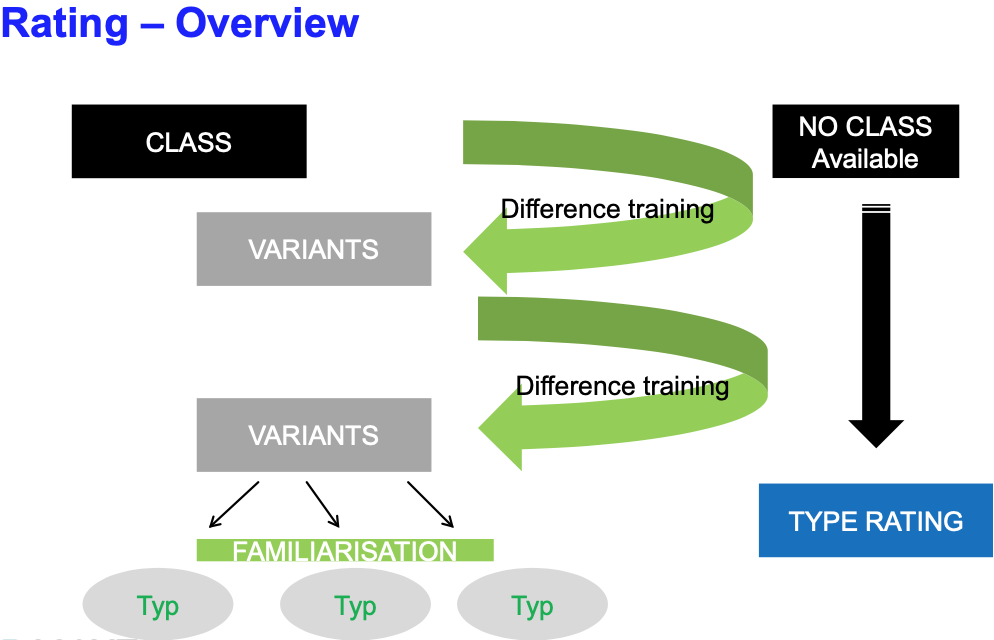
\includegraphics[width=9cm]{Images/Ratings.png}
\end{center}
\underline{\textbf{Revalidation of Licenses}}
\begin{itemize}
    \item Classes
    \begin{itemize}
        \item Single-engine piston-engine aircraft generally valid for 2 years. 12 FH experience, 6 as Pilot in Command (PIC). 12 take-offs/landing and a 1 hour training flight with instructor
        \item Multi-engine piston-engine A/C valid generally for 1 year 
    \end{itemize}
    \item Type Ratings
    \begin{itemize}
        \item All aircraft with 2 pilots 
        \item All multi-engine aircraft with 1 pilot and turboprop or jet-engine 
        \item All single-engine A/C with 1 pilot and jet-engine
    \end{itemize}
    \item Extension of Licenses (variety of extensions)
    \begin{itemize}
        \item Aerobatics 
        \item Towing of gliders and banners 
        \item Night flight 
        \item Mountain flight authority for skiers and/or wheels 
        \item FI-Flight Instructur / CRI-Class Rating Instructor 
    \end{itemize}
    \item Radio Licenses: English Language Proficience (ELP) Check required in order to use the aeronautical radio service (lvl 4/6 - 4 years. lvl 6/6 no expiration)
\end{itemize}
\underline{\textbf{VLL Par. 22 - Documents on Board/Air Worthiness Req.}}
\begin{itemize}
    \item Registration Certificate (Eintragungszeugnis)
    \item Certificate of Airworthiness (Lufttüchigkeitszeugnis) or air permit with annex ``scope of uitilization'' (Zulassungsbereich des Luftfahrzeuges) in flight handbook
    \item (Valid airworthiness review certificate or the valid verification of the airworthiness checks)
    \item Noise Certificate (Lärmzeugnis) (if required)
    \item Proof of third party liability insurance on ground and if required for liability insurance agains passengers 
    \item Concession for Aircraft Station (for radioelectric reception and transmission equipment)
    \item Aircraft Flight Manual 
    \item Flight Book (clearance certificates as well)
    \item Checklist issued by manufacturer or check list created by the owner  
\end{itemize}
\underline{\textbf{Additional Requirements for VFR (Visual Flight Rules) Flight Planning}}
\begin{itemize}
    \item Instrument Flight Rules (see Aircraft Operations): Weather, NOTAM, OFP 
    \item VFR
    \begin{itemize}
        \item DABS (Daily Airspace Bulletin Switzerland) is required 
        \item AIP (Aeronautical Information Publication) for VFR maps, Airport information and basic info 
        \item AIC (Aeronautical Information Circular): Publishes changes which affect aviation safety, e.g. new rules (included in NOTAM)
    \end{itemize}
\end{itemize}
\underline{\textbf{Air Traffic Control - Submission of Flight Plans}}
\begin{itemize}
    \item Submission required for 
    \begin{itemize}
        \item IFR Flights 
        \item VFR-Night Flights (NVFR)
        \item VFR-flights with landings in other countries 
        \item Zurich and Geneva Airport 
    \end{itemize}
    \item Optional for VFR-flights, however facilitates search and rescue operations 
\end{itemize}
\underline{\textbf{General Traffic Rules (ICAO Annex 2/VVR)}}
\begin{itemize}
    \item Swiss traffic rules apply to all aircraft within Swiss territory, as well as abroad, unless other rules apply
    \item A commander must keep to the rules, whether at the controls or not and can only deviate from these in emergencies 
    \item A commander (PiC) must be prepared for the flight, especially flying outside of the aerodrome vicinity and/or as IFR flight he must check the weather, must plan with an alternate aerodrome and have sufficient reserve fuel (Jet/turboprop 30 min /others 45 min)
    \item Anyone feeling sick, tired or under the influence, is not allowed to be an active member of the crew 
    \item Maximum speed: Under FL 100, 250KTS (460km/h). VFR over FL200 are not allowed 
    \item During flight, objects/liquids can only be dumped with the permission from BAZL/FOCA (except ballast in the form of water or sand/in emergencies/for rescue missions/tow ropes or under carriages at airfields/wind drift indicators for parachute jumpers, wind indicators for Landings or reporting bags for air races)
\end{itemize}
\begin{center}
    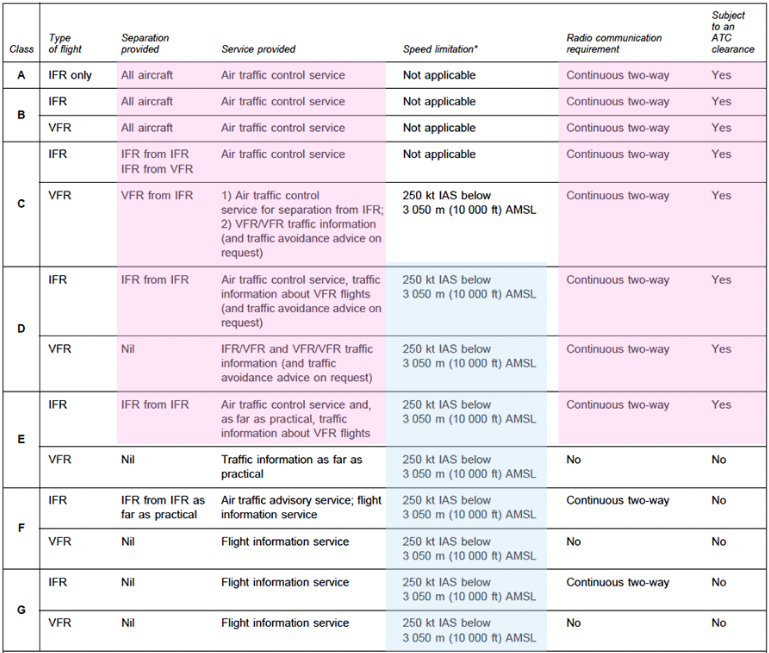
\includegraphics[width=9cm]{Images/Airspace controlled-uncontrolled.png}
\end{center}
\underline{\textbf{Airspaces - CH (Slide 30), UK (Slide 31), US (Slide 32)}} \\ \\
\underline{\textbf{Requirements for VFR}}
\begin{itemize}
    \item Day: Beginning of the civil twillight and the end of the civil twillight (30 min before sunrise and 30 min after sunset), (6 degrees)
    \begin{itemize}
        \item Visibility
        \begin{itemize}
            \item Zone G (2000ft AGL): 1.5-5 km 
            \item Under FL100 (2'000ft $<$ H $<$ 10'000 ft): 5km 
            \item Above FL100: 8 km
        \end{itemize}
        \item Distances from Clouds
        \begin{itemize}
            \item G: outside of Clouds 
            \item Above G: 300m above and below, 1.5 km in front 
        \end{itemize}
        \item Night-VFR, Special VFR (within control zones and reduced weather conditions) and Controlled-VFR: Special Requirements
        \item Airspace G: 600m/2000ft AGL: 1.5km allowed if aircraft speed allows a $180^\circ$ turn with visibility, and helis may fly less than 1.5km if obstacles are recognised and other traffic is avoided
    \end{itemize}
\end{itemize}
\underline{\textbf{Semi-circle Rule}}
\begin{center}
    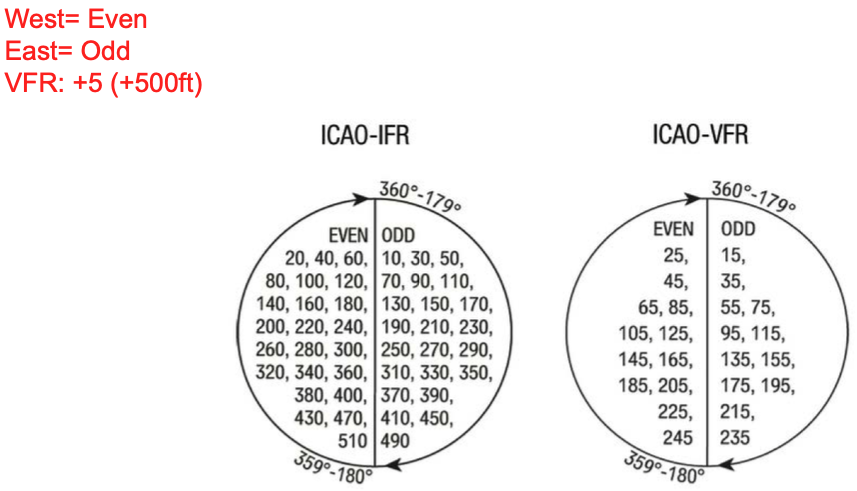
\includegraphics[width=8cm]{Images/Semicircle_Rule.png}
\end{center}
\underline{\textbf{Operation near Airfield}}
\begin{itemize}
    \item Observe other traffic 
    \item Integrate into the traffic flow 
    \item Fly curves to the left (left-hand)
    \item Start and land against the wind 
\end{itemize}
\underline{\textbf{Minimum flight altitudes}}
\begin{itemize}
    \item Uninhabited areas or forrest: height 150m, radius 150m 
    \item Over heavily populated areas and over viewing areas of events: height 300m, radius 600m
    \item Over water: h 150m
\end{itemize}
\underline{\textbf{Flight Hazards, Restrictions, Prohibited Areas}}
\begin{itemize}
    \item Danger Areas (LS-D, limited in time and Scale): Should not be flown through during active periods (often army shooting practice). Options: Over- or underfly resp. circumnavigate it/ alternatively, request permission on ATC for crossing the area.
    \item Restricted Areas (LS-R): Must not be flown through during active phases (WEF or test flights)
    \item Prohibited Areas (LS-P): General flying ban (not in CH applied)
\end{itemize}
\underline{\textbf{Altimeter Settings}}
\begin{itemize}
    \item QNH: Elevation set at sea-level, shows above sea (MSL)
    \item QFE: Altimeter shows zero at airfield (pressure at airfield elevation)
    \item QNE: Standard pressure (1013 hPa) for flight level (FL) display
    \item VFR/IFR, In closely controlled zone or a control zones (IFR/VFR): Set to QNE if aircraft is above transition altitude (TA)
    \item VFR/IFR In closely controlled zone or a control zones (IFR/VFR): Set to QNH when below transition level (TL)
    \item VFR, Outside of controlled zone: Over 900m (3000ft): QNE (FL) 
    \item VFR, Outside of controlled zone: Below 900m: QNH 
    \item Gliders, Balloons: QNH 
\end{itemize}
\underline{\textbf{Collision Avoidance}} \\ \\ 
An aircraft with right of way (Rechtsvortritt) maintains its course and speed (also converging traffic). When head-on, alter course to the right. When overtaking, alter course to the right
\underline{\textbf{Collision Avoidance/Priorities from highest to lowest}}
\begin{enumerate}
    \item Aircraft in distress 
    \item Balloon 
    \item Glider under Tow
    \item Glider 
    \item Air ship / zeppellin 
    \item Heli 
    \item Aeroplane and microlight
\end{enumerate}
\underline{\textbf{Collision Avoidance/Landing}}
\begin{itemize}
    \item Landing Aircrafts take precedence 
    \item Lower flying aircrafts take precedence 
    \item Gliders take precedenced over powered aircrafts 
    \item An aircraft in an emergency situation always takes precedence
\end{itemize}
\underline{\textbf{Collision Avoidance/On Ground}}
\begin{itemize}
    \item Starting aircraft takes precedence over rolling aircraft 
    \item On ground, rolling aircraft must stop if they are on a collision course, or turn to the right 
    \item On the ground, right of way applies 
\end{itemize}
\underline{\textbf{Emergency vs Urgency}}
\begin{itemize}
    \item If an A/C is in an emergency situation, the commandor is no longer bound by the regulations and can deviate from these 
    \item An emergency or an Urgency can be declared. For emergencies, immediate assistance from the ATC is needed 
    \item Emergency:
    \begin{itemize}
        \item SOS (morse)
        \item 3 x MAYDAY 
        \item Red rockets (in short intervals)
        \item Squawk 7700 (on Transponder)
    \end{itemize} 
    \item Urgency
    \begin{itemize}
        \item 3 x PANPAN 
        \item Switch landing lights on- and off 
        \item Squawk 7600 for communication loss 
        \item Squack 7500 for hi-jacking
    \end{itemize}
\end{itemize}
\underline{\textbf{Violence on Board/Responsibility of the Commander}}
\begin{itemize}
    \item Regarding Passengers:
    \begin{enumerate}
        \item Passengers on board are under the control of the commander 
        \item They are obliged to observe flight safety rules and maintain order and discipline on board 
        \item After an unsuccessful warning, the commander is entitled to offload a passenger who does not follow instructions 
    \end{enumerate}
    \item Beginning and Ending 
    \begin{itemize}
        \item The control of the commanding officer over the passengers begins with the closing of the A/C before the journey
        \item It ends with the opening of the A/C after completion of the journey or journey segment, and after emergency landings or accident from the time when care of the passengers is taken over from others 
    \end{itemize}
\end{itemize}
\underline{\textbf{Standard Time UTC}}
\begin{itemize}
    \item In aviation, everything runs in UTC (not time zones). Previously know as GMT (Greenwhich Mean Time)
    \item UTC is independent of summer or winter time 
    \item CH: UTC+2
\end{itemize}
\newpage
\section{Business Aviation}
\underline{\textbf{Key Drivers}}
\begin{itemize}
    \item Corporate Profits
    \item General Economic Growth 
    \item Increases in Wealth 
    \item Aircraft Product Innovation, e.g. increase in range, VLJs
    \item Alternatives to full ownership - membership programs, fractionals, on demand charters 
    \item New Business Models
\end{itemize}
\begin{center}
    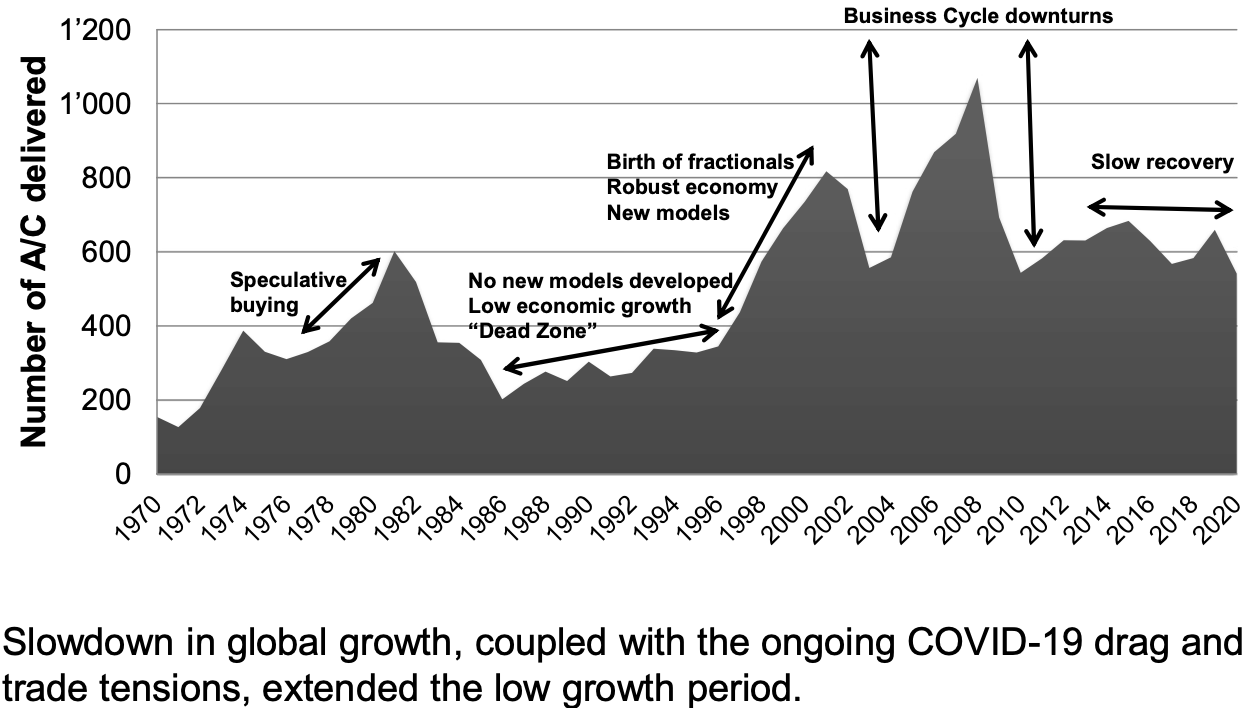
\includegraphics[width=9.2cm]{Images/Global_Business_Jet_Deliveries.png}
\end{center}
\underline{\textbf{Primary Motivators of Use}}
\begin{itemize}
    \item Efficiency - EU average time savings 127min 
    \item Productivity (153 min per trip/employee = 15\% increase)
    \item Airline Schedule Inadequacy 
    \item Security 
    \item Privacy
    \item Control / Agility 
    \item Luxury / Comfort / Reduced Hassle 
    \item Cost Savings (for large groups, EU 15M hotel costs)
\end{itemize}
\underline{\textbf{Customers}}
\begin{itemize}
    \item End Users 
    \begin{itemize}
        \item Corporations 
        \item Wealthy Individuals 
        \item Governmental VIPs 
        \item Medical and Insurance Companies (120'000 departures annually EU)
    \end{itemize}
    \item Intermediaries (Fly Commercially and have an AOC)
    \begin{itemize}
        \item Charter Operations 
        \item Fractional Operations 
    \end{itemize}
\end{itemize}
\underline{\textbf{Business Aviation Operating Models}}
\begin{itemize}
    \item Commercial (Intermediaries) (600-1200 FH annually): Over 700 in EU. 80\% in EU have fewer than 5 A/C
    \begin{itemize}
        \item Aircraft flown for Business purposes by having an AOC 
        \item Air Charters (Air Taxis), Fractional Operators 
    \end{itemize}
    \item End User 
    \begin{itemize}
        \item Corporate (200-600 FH annually): Non-commercial operations with professional operations with prof. crews employed to fly the aircraft (corporate fleets)
        \item Owner-operated (150-250 FH annualy): Aircraft flown for business purposes by the owner of the A/C
    \end{itemize}
\end{itemize}
\underline{\textbf{Average Annual Aircraft Spend} - see slide 12}\\
\underline{\textbf{Direct Operating Costs = 10\% of ownership costs}} \\ \\
\underline{\textbf{Business Aircraft Segmentation by Units}}
\begin{itemize}
    \item Installed base is now dominated by large aircraft (shift from light to heavy). Longer distances, bigger cabins, prestige are causes for this 
    \item Citations/Cessna and Bombardier account for 53\% of the installed base
\end{itemize}
\underline{\textbf{OEM Product line key drivers}}
\begin{itemize}
    \item Size matters - flagship effect (Gulfstream = ``Rolls-Royce'') 
    \item Leverage installed base 
    \item Clear value proposition (PC-21 from Pilatus has features others do not have)
    \item Time to market 
    \item Program complexity - risk factors 
    \item Commercial Impact 
    \item Aftermarket Services 
\end{itemize}
\underline{\textbf{New Aircraft Development}}
\begin{itemize}
    \item New aircraft programs can either be derivative or clean-sheet designs 
    \item Clean-design aircraft involves higher costs (designing, building and certifying)
    \item High cost of full program execution: Design, development, production, entry into service 
    \item Ability to provide excellent after market services, e.g. strong MRO network 
\end{itemize}
\underline{\textbf{European Flight Patterns}}
\begin{itemize}
    \item The network of airport pairs linked by business aviation has over 25'000 links, three times as many links as the scheduled network (top 30 city pairs only cover 5\% of the links)
    \item 45\% of business aviation flights are under 450km (most frequented city pairs are: Nice-Paris and Paris-Geneva)
    \item The most common range is 250-350km
    \item Airports served are mostly not the large ones due to conflicts with service airlines and available slots
\end{itemize}
\underline{\textbf{COVID-19}}
\begin{itemize}
    \item Even though COVID-19 had a large impact on aviation, business aviation particularly has recovered quite well. Record numbers in 2021. 
    \item Reasons for Recovery 
    \begin{itemize}
        \item Accessibility/flexibility - serves destinations to which airlines have still not resumed operations
        or do not offer sufficient frequency
        \item Safer - less exposure to the virus versus commercial flights
    \end{itemize}
\end{itemize}
\begin{center}
    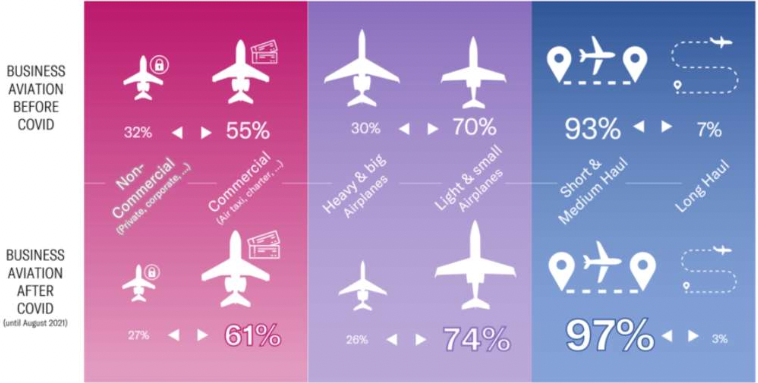
\includegraphics[width=9cm]{Images/Winners_and_Losers.png}
\end{center}
\underline{\textbf{Dedicated Business Aviation Airports}}
\begin{itemize}
    \item No conflict with commercial airlines
    \item No queues in the air or on ground
    \item Access to hangars 
    \item Ramp access
    \item No security check (less rigid)
    \item Speedy immigration procedures
    \item Discretion 
    \item Key BA Airports
    \begin{itemize}
        \item Teterboro, NJ - largest Worldwide
        \item Paris Le Bourget - larges in EU 
        \item London Fanborough
        \item London Biggin Hill
    \end{itemize}
\end{itemize}
\underline{\textbf{Summary - Business Aviation Market}}
\begin{itemize}
    \item Concentration 
    \begin{itemize}
        \item Fleet size $>$ 22'000 A/C
        \item 81\% of fleet in top 10 countries (US, MX, BR, CA, DE, VEN,CN,UK,AT,AUS,ARG)
        \item 62\% of fleet in the US 
        \item Top 20 airports Europe - 40\% share by top 5 airports (4 in FR and CH)
    \end{itemize}
    \item Fragmentation
    \begin{itemize}
        \item $>$ 280 A/C in fleet, $>35$ in production, 14 in development 
        \item Europe 700 operators, 80\% $<$ 5 A/C per fleet 
        \item Europe top 30 city pairs cover only $5\%$ of airport links 
    \end{itemize}
    \item Market drivers: Economy and Innovation 
    \item Trand to larger aircraft - 62\% unit share, 87\% share value
\end{itemize}
\underline{\textbf{Primary Businesses}}
\begin{itemize}
    \item Airframe, Engine and Parts Manufacturers (21.6 B\$)
    \item Completions \& Refurbishements Providers (4.7B\$)
    \item Charter \& Fractional Operators (16.3\$)
    \item Fleet Management (2.4 B\$)
    \item Fixed Base Operators (FBOs) / Handling (13.7B\$) 
    \item Maintenance, Repair and Overhaul Providers (MROs) (13.2 B\$)
\end{itemize}
\underline{\textbf{Maintenance}}
\begin{itemize}
    \item Key drivers: Growing fleet, aging aircraft (17.1 years avg. fleet age), uitilization
    \item Maintenance Center Types: OEM owned Service Center, Independent Service Center with OEM license, or without OEM license 
    \item High entry barriers: Infrastructure, Capabilities, Licensed Mechanics 
    \item Key Players: OEMs or OEM licensed service centers (Jet Aviation, Standard Aero, Duncan, West Star, ...)
\end{itemize}
\underline{\textbf{Completions}}
\begin{itemize}
    \item 503 (417 Narrowbody, 86 widebody) A/C in use worldwide (318 Boeing, 159 Airbus, 26 other)
    \item 7 to 12 VIP completion opportunities per year, incl. conversions (small and competitive market)
    \item Key Drivers: Green deliveries (empty aircraft, not painted), Airline Conversions
    \item High entry barriers: Infrastructure, Capabilities, Licensed Mechanics, Craftsmen, Good reputation, strong brand 
    \item Key players: Jet Aviation, Lufthansa Technics, GDC Technics 
\end{itemize}
\underline{\textbf{Aircraft Accesibility}}
\begin{itemize}
    \item Full ownership (with following alternatives)
    \item Branded Charter 
    \item Fractional Ownership 
    \item Jet Card Programs 
    \item Air Taxis 
    \item Memberships 
\end{itemize}
\underline{\textbf{Aircraft Management}}
\begin{itemize}
    \item Full ownership
    \item Own flight department vs. third-party manager 
    \item Low entry barriers 
    \item Highly fragmented market 
    \item Key players: Luxaviation, Jet Aviation, Solairus - each over $>200$ A/C in fleet 
    \item Benefits: Turnkey Solution - time saving and peace of mind, Economies of Scale, Charter Income, Finance, Tax benefits, Safety 
\end{itemize}
\underline{\textbf{Charter \& Fractionals}}
\begin{itemize}
    \item Charter 
    \begin{itemize}
        \item Key driver - economic activity 
        \item Pay as you go, upfront payment 
        \item Depending on where A/C located, repositioning costs can be high 
        \item Jet Card programmes start at 25 hours per year
        \item Highly fragmented market (4500 business jets available, 1300 charter companies)
        \item Demand for business jet travel in the charter market is returning after global pandemic  
    \end{itemize} 
    \item Fractionals 
    \begin{itemize}
        \item Similar to timeshare on a property 
        \item Shares start at 1/16th of a private jet 
        \item Flate hourly rate for time in the air 
        \item No charge for positioning costs 
        \item Typically five year contract (option to terminate in three)
        \item Netjet largest market player (70\%)
        \item Fractional Fleet down 
        \item Major Market consolidation (already tough to get into)
    \end{itemize}
\end{itemize}
\underline{\textbf{Fixed Based Operations (FBO) and Handling}}
\begin{itemize}
    \item Key drivers: Departures (EMEA \& Asia) and Fuel Gallons (USA, service included)
    \item Key Players: Signature/Landmark, Jet Aviation, Execujet, German Aviation Services
    \item Services: Handling, Fuel, De-Icing, GSE, Water and Toilet, Lounges, Catering, Ground Transport, Hangarage, Ramp Parking, A/C Cleaning, Line Maintenance
\end{itemize}
\underline{\textbf{Operating Models for FBO and Handling}}
\begin{itemize}
    \item Supervision: Own meet \& greet, crew briefing service only, operational services mainly outsourced 
    \item Ground Handling: Offices \& lounge, A/C, crew and passanger handling, operational services insourced
    \item Full Service FBO: Comprehensive service portfolio, control over terminal and ramp, Additional revenues through fuel, hangarage, and providing services for customs, immigration and security check 
\end{itemize}
\underline{\textbf{Regional Differences - USA vs EMEA \& Asia}}
\begin{itemize}
    \item USA 
    \begin{itemize}
        \item Liberal market (dedicated bizav airports, level playing field for providers)
        \item Two business modles (large chanis or single site providers)
        \item Fuel, Hanger, GSE (integral part of FBO)
        \item Ramp/Land Controlled by FBOs (no man in the van competition)
        \item More land available (construction and facilitiy development easier)
    \end{itemize}
    \item EMEA \& Asia 
    \begin{itemize}
        \item Closed Markets (airports focus on airlines, different concessions for FBO, GH, GSE Fuel)
        \item Many different busines models (everyone provides all services without concession - low entry barriers)
        \item Fuel, Hanger, GSE (separate items)
        \item Ramp/land controlled by airport (different competitors/models for FBO)
        \item Space restrictions (lack of space, most available land dedicated to airline operations or freight)
    \end{itemize}
\end{itemize}
\underline{\textbf{Primary Businesses - Summary}}
\begin{itemize}
    \item Challenging market conditions
    \item Several alternatives to full business A/C ownership exist that extend the benefits of private jet travel to many users - charter, fractionals, membership cards 
    \item FBO/Handling: US focus on fuel vs. ROW (rest of world) a la carte services 
\end{itemize}
\underline{\textbf{General Market Challenges}} \\ 
Lack of common legal definition and standards of business aviation causes confusion and dilutes focus
\begin{itemize}
    \item Emerging Markets 
    \begin{itemize}
        \item Overcome cultural and image hurdles 
        \item Unfavourable Tax Situation 
        \item Legal complexity 
        \item Contraints on part imports and exports on foreign registered aircraft 
        \item Approvals and licenses: lengthy and painful process 
    \end{itemize}
    \item Maturing Markets 
    \begin{itemize}
        \item Congestion at primary airports - increasing competition with airlines for slots 
        \item Increasing security measures degrade convenience 
        \item Regulatory environment (adds complexity and costs) - will drive restructuring activities 
        \begin{itemize}
            \item Certification 
            \item Operations 
            \item Tax and fees 
            \item Environmental Compliance 
        \end{itemize}
    \end{itemize}    
    \item Maintenance Challenges
    \begin{itemize}
        \item Number of aircraft types increasing - 280+ in fleet 
        \item Maintenance Programs are changing (Aircrafts more reliable, longer intervals, fewer man hours per task)
        \item OEMs taking greater share of aftermarket (PBTH (Pay by the hour) programs, Lower parts discounts, extended warranty)
    \end{itemize}
    \item Operator Challenges 
    \begin{itemize}
        \item A small commercial business aviation operator has to comply with the same regulations and standards as an airline
        \item Critical mass required to achieve sustainable profitability in an increased complex environment
    \end{itemize}
    \item FBO hand Handling Challenges 
    \begin{itemize}
        \item Consolidation of small operators into large AOC companies leads to
        \begin{itemize}
            \item Bundling volume to leverage buying power
            \item Fleet operators signing up with network solution providers for
            regions and countries
        \end{itemize}
        \item Consolidation into larger FBO Chains 
        \item Single location providers looking for “network” partnerships i.e. Air Elite, Signature Select, etc
    \end{itemize}
\end{itemize}
\underline{\textbf{Future}}
\begin{itemize}
    \item Younger Clientele: Users are becoming younger. Driven by their lifestyles, they expect choice, personalisation, price transparency and ease of access
    \begin{itemize}
        \item Technology: Innovation makes experience faster, easier, more accesible and transparent
        \item Moving away from Ownership: Renting models, similar to Airbnb, Uber 
        \item Sustainability: Environmental sustainable solutions 
    \end{itemize}
\end{itemize}
\underline{\textbf{Sustainable Aviation, Technology: See Slides}} \\ \\ 
\underline{\textbf{Summary: Market Trends and Challenges}}
\begin{itemize}
    \item Maintenance: 280+ A/C types to maintain, more reliable A/Cs, OEMs insourcing aftermarket services 
    \item Operators: Small fleet, high costs 
    \item FBO/Handling: Single Providers struggling 
    \item COVID-19: Trend to smaller A/Cs impacts corporate profits negatively 
    \item Main message: From fragmentation to consolidation to achieve critical mass 
    \item Future: Business aviation be undergoing a paradigm shift, prompted by a combination of technological disruption and societal expectations
\end{itemize}
\newpage
\section{Air Traffic Control (ATC)}
\underline{\textbf{The main tasks of ATC}}
\begin{itemize}
    \item Avoid collisions in the air 
    \item Avoid collisions on the ground 
    \item Ensure an orderly and expeditious flow of traffic 
    \item Provide flight information services (weather data)
    \item Provide alerting services and support search and rescue crews 
\end{itemize}
\underline{\textbf{Standard Minimum Separation}}
\begin{itemize}
    \item Horizontal distance: 5 Nautical Miles (9000 m) (for approaches: 3 NM)
    \item Vertical distance: 1000ft (300m)
\end{itemize}
\underline{\textbf{Elements of Air Traffic Control}}
\begin{itemize}
    \item Tower Control 
    \item Approach \& Departure Control 
    \item Are Control
    \item Air Traffic Flow and Capacity Management
    \item Flight Information Services 
    \item Military Air Traffic Control 
\end{itemize}
\underline{\textbf{Tower Control}}
\begin{itemize}
    \item In control towers (TWR), air traffic controllers monitor traxiing manoeuvers, takeoffs and langings 
    \item They oversee traffic in the immediate vicinity of the airport, i.e. the control zone (CTR) of approx. 20km around the airport 
    \item The tower air traffic controllers also integrate into the often dense traffic of an airport the small A/Cs and helis flying according to visual flight rules (VFR)
    \item Working Positions: 
    \begin{itemize}
        \item ADC: Aerodrome Controller - issues landing and takeoff clearances and clearances in control zones
        \item GND: Ground Manoeuvering - lead A/C on ground
        \item CLD: Clearance Delivery - at international airports. A/C receive transponder codes for final clearances from CLD 
        \item AMS: Apron Management Service - gives clearance for engine start, pushback, gives permission and transfers responsibility to GND 
    \end{itemize}
\end{itemize}
\underline{\textbf{Approach \& Departure Control}}
\begin{itemize}
    \item Approach (APP) air traffic controllers manage the arriving and departing A/C flying according to IFR within a specific section of the control zone and terminal control area (TMA) (region around airport 60km)
    \item Approach controllers manage the traffic climbing to upper airspace airways and descending traffic that leaves these airways toward the airport 
    \item In case of dense traffic, aircraft waiting to land be directed into holding circuits (holdings)
    \item Working Positions:
    \begin{itemize}
        \item DEP: Departure Controller 
        \item APW: Approach Controller East 
        \item APE: Approach Controller West
        \item FIN: Final Controller 
        \item CAP: Coordinator for the Approach Sector 
    \end{itemize}
\end{itemize}
\underline{\textbf{Area Control (Enroute Control)}}
\begin{itemize}
    \item Area control or en-route services ensure the saftey and efficiency of traffic moevements through the airways 
    \item In Switzerland, the controlled area includes parts of neighbouring France, Germany, Italy and Austria from 7'000 ft to 66'000 ft
    \item The airspace that skyguide controls at the the heart of Europe is the densest and most complex on the continent 
    \item In order to safely and efficiently control and monitor the air traffic, the area is split into various control sectors with clearly defined lateral and horizontal boundaries 
\end{itemize}
\underline{\textbf{Enroute Controllers (RE, RP, RC)}}
\begin{itemize}
    \item RE: Radar Executive (talks to A/C and controller to take responsibility)
    \item RP: Radar Planner (short-time future (15min) predictions for A/C route and solves potential conflicts)
    \item RC: Radar Coordinator (coordinates between different sectors (N,E,S,W)) - used for conflicts (extra pair of eyes)
    \item Tools and Procedures: Voice-control (RE), RP works on Systems with Radar Picture (Flight, callsign, type of equipment Wake Turbulence Category) - no more tel. required 
\end{itemize}
\underline{\textbf{Radar Labels}}
\begin{itemize}
    \item Update every 5 seconds 
    \item GXXX (ground speed)
    \item rls (equipment)
    \item 260 (Flight Level)
    \item V KOR32 (Coordinate to which flight level it should climb)
\end{itemize}
\underline{\textbf{Flight Information Service}}
\begin{itemize}
    \item VFR Flights 
    \item Parachute Drops 
    \item Special Flights
    \item Gliders and Balloons 
\end{itemize}
\underline{\textbf{Mixed Traffic in the Zurich TMA}}
\begin{itemize}
    \item Arrivals (Green)
    \item Parachute / Special Callsigns (Orange)
    \item Below Airspace (V in yellow)
    \item Departures (Blue)
\end{itemize}
\underline{\textbf{Tasks of Military Air Traffic Control}}
\begin{itemize}
    \item When working in the ADDC, Air Traffic Controllers are ``fighter controllers''
    \item They also manage all military aircraft in transit flights within CH. Like civil air traffic controllers, fighter controllres monitor the airspace on radar consoles 
    \item The ADDC also helps the air police with the critical task of recognising aircraft with a questionable identity 
    \item Specific deployment procedures are used in air defence training, and the protection of specified areas, e.g. WEF
\end{itemize}
\underline{\textbf{Conventional Air Navigation Technology}}
\begin{itemize}
    \item NDB for Transit 
    \item VOR for $360^\circ$
    \item ILS with localiser (lateral direction) and tower for glide path 
\end{itemize}
\underline{\textbf{GPS}}
\begin{itemize}
    \item Aircraft based augmentation Systems (ABAS)
    \item Spaced based augmentation systems (SBAS)
    \item Ground based augmentation systems (GBAS)
    \item RNP = Required Navigation Performance, RNP1 is for arrival and initial, intermediate and missed approach as well as departure navigation applications
\end{itemize}
\underline{\textbf{New possibilities with Satellite Navigation}}
\begin{itemize}
    \item Curved flight paths 
    \item Less steep approach profiles 
    \item Continuous Descent OPS 
    \item Higher Navigation Precision 
\end{itemize}
\underline{\textbf{ATC today and tomorrow}}
\begin{itemize}
    \item Virtual Center Concept 
    \item Virtual and Central Services 
    \item Remote Tower Systems 
    \item Integration of Drones in Airspace Management 
\end{itemize}
\newpage
\section{Airline Industry \& Business Models}
\underline{\textbf{Airline Industry}}
\begin{itemize}
    \item ...is a complex industry 
    \item ...has been developed especially after deregulation 
    \item ...is a cyclical industry 
    \item ...'s traffic volume is strongly related to world GDP 
    \item ...'s cost are 65-90\% fixed costs 
    \item ...shows decline of yield per seat-km (RPK)
    \item ...shows better productivity, worse margins of only 1-8\%
    \item ...has developing networks: Point-to-Point (regulated market), Hub-and-Spoke (deregulated market), networks (alliances, global market)
\end{itemize}
\underline{\textbf{Network Airline (Hub \& Spoke)}} = Full Service Carriers (FSC), Network Carriers, Legacy Carriers or Flag Carriers, Traditional Airline, Mainline Carrier
\begin{itemize}
    \item 2 types: Traditional/Lufthansa (Airline handles all aspects), 2. Aviation Busines Model Swiss (Airline handles mainly Flight Operations)
    \item \textbf{Advantages of H\&S Model}:
    \begin{itemize}
        \item Connecting many local regions which would otherwise not be served
        \item Many connections
        \item S-Curve Concept (much higher revenue with higher capacity or frequency)
        \item Large and attractive network
        \item Hub dominance (slots, gates)
        \item Advantage in the reservations
        system (Comp. Res. System/CRS)
        \item Economies of density (smaller routes can be covered by larger aircraft = lower costs)
        \item Feeding Shorthaul-Longhaul (vs.)
    \end{itemize}
    \item \textbf{Weaknesses}
    \begin{itemize}
        \item Waves at the hub (Pax and therefore Crew/personell)
        \item Seducement for “hub economies”/ sales at variable costs (Bait prices to the hub...)
        \item Optimal connection leads to “waves” $\rightarrow$ higher personnel requirement \& hub at the limit
        \item Short transfer times $\rightarrow$ domino effect
        \item H\&S $\rightarrow$ additional operative costs (up to +45\%)
        \item High “Overhead” costs (one airline fits all...)
        \item Flights from “origin to destination” via hub take longer
        \item Long ground times for network (A/C utilisation low)
        \item “Primary Airports” have higher charges
        \item Overlapping structure (competition)
        \item Demand for direct flights from PAX (time)
        \item New airspaces allow more direct flights (chances)
        \item Overloading and security checks at “Primary Airports”
        \item Competitors have more efficient aircraft
    \end{itemize}
\end{itemize}
\underline{\textbf{Low Cost Carrier}} (Low Fare Airline, No Frill Airline). Main Motivation: First LCC Airline: Southwest - has never experienced financial loss. Net profit in the region of 18-24\%
\begin{itemize}
    \item Global Market Share: Stablilises at 35\% 
    \item Europe: From 17\% in 2005 to 32\% in 2013. Ryanair, Easyjet and Alitatlia 
    \item Strategy: 
    \item Advantages of LCCs:
    \begin{itemize}
        \item Lower airport charges, faster turnaround times, less air traffic control-related delays 
        \item Better fleet utilisation 
        \item Lower complexity, higher capacity utilisation 
        \item Cheaper aircraft financing, lower maintenance and training cost, simpler swapping around of flight and maintenance staff 
        \item Lower distribution costs, lower complexity 
        \item Lower anciliarry costs, less complexity, additional revenues 
        \item Higher employee productivity (incentives and variable proportion of salary)
    \end{itemize}
    \item Activity Systems (Michael Porter)
    \begin{itemize}
        \item Activities complement one another in ways that create real economic value. One activity's cost is lowered because of the way others are performed
        \item No catering on board means no need for cleaning and thus allows a turnaround time of under 30 minutes
    \end{itemize}
    \item LCCs generate new customers (new demand, people who would otherwise not have traveled, otherwise by car or rail)
\end{itemize}
\underline{\textbf{Charter Airlines}}
\begin{itemize}
    \item Four basic types: 
    \begin{itemize}
        \item Vertical Integrated Organisation, tour operating travel agents, hotels etc. (TUIFly)
        \item Independents (Condor)
        \item Subsidiairies of network carriers (Edelweiss)
        \item Scheduled Airlines (SWISS)
    \end{itemize}
    \item Vertically Integrated: Parent company (tour operator) takes over 70-90\% of the capacity 
    \item As tickets are sold through mother company/tour operators and the destination is not regularly flown, a high SLF results
    \item Comparison to LCCs: 37\% of all travel destinations are offered by LCCs. FLights under 2.5h are handled by LCCs (one-way, flexibility and frequency)
    \item Advantage of Charter: Lower unit costs
    \begin{itemize}
        \item Larger A/C 
        \item Longer Sectors 
        \item High SLF 
        \item Higher Labour Productivity 
        \item Lower Insurance Costs 
        \item Lower A/C leasing costs 
        \item Lower Administration and Finance Costs 
    \end{itemize}
\end{itemize}
\underline{\textbf{Sales strategies/yield management}} (Revenue Mgmt, Capacity Mgmt, Dynamic Pricing)
\begin{itemize}
    \item Airlines maximise revenue through 
    \begin{itemize}
        \item Variable Prices 
        \item Seating Offer (Aircraft Size)
        \item Booking Figures
    \end{itemize}
    \item Turnover (revenue) is increased by 3-7\% and profit by 50-100\%
    \item Prices with LCCs and FSCs generally increase shortly before flight (given SLF is high)
    \item With Charter FLights, they withdraw them shortly before as quotas sold to travel agents and tour operators at an early stage
\end{itemize}
\underline{\textbf{Regional Airline (Feeder): Definition}}
\begin{itemize}
    \item Fewer than 100 seats and distances flying up to 800 km (turnover below 100M USD)
    \item Normally a subsidiary of an NWC (50\%), and are dependent of these feeders/capacity providers
    \item 70\% Hub to Non Hub routes
    \item Operate from smaller airports, with smaller aircraft (better financially)
\end{itemize}
\underline{\textbf{Longhaul - Business Only}}
\begin{itemize}
    \item Only business seating and corresponding service (48-56 seats)
    \item Larger overhead bins, PC-Laptop Connections, Fast Track Counter, VIP Service 
    \item Popular for business customers (only like-minded people on board)
    \item Private Jet Feeling 
    \item Only possible on selected routs 
    \item Sufficient business passengers required 
    \item However, do not last long: EOS, MaxJet, Silverjet, PrivatAir (all bankrupt or OPS suspended)
\end{itemize}
\underline{\textbf{Trends}}
\begin{itemize}
    \item Emerging Markets increasing (Asia, i.e. China and India) - 2/3 of population of emerging markets will take a trip in 2032
    \item Strategically different approaches between Boeing \& Airbus 
    \begin{itemize}
        \item Boeing: Smaller and more A/C are needed as market becomes fragmented (=new routes and more direct flights)
        \item Boeing services: Lower cabin pressure, more humidity, 50\% larger windows, virtually larger cabins 
        \item Airbus: Markets have to consolidate, which require larger aircraft 
        \item Airbus services: Bars, casinos, sleeping areas, shower rooms (20\% lower operational costs)
    \end{itemize}
    \item Faster: Boom Supersonic 
    \item Greener: Electric/Hybrid 
\end{itemize}
\underline{\textbf{Strategies for Success}}
\begin{itemize}
    \item Clear strategy/positioning 
    \item Activity System 
    \item Adapted Networks/alliances 
    \item S-Curve (Flying every day)
    \item Slots/Hubs dominance (gates)
    \item Eco of Densities (Seating/Aircraft Sizes)
    \item Ideal Capacity Efficiency
    \item Low Cannibalization 
    \item Flat waves at the hub 
    \item Freq. Flyer Program 
    \item Larger Aircraft 
    \item Longhaul 
    \item Secondary Airport 
    \item Short turnaround times = high A/C utilization 
    \item Direct Flights 
    \item Standardized Fleet 
    \item Yield Management (Revenue)
    \item Direct Sales (Website)
    \item Few ``Frills'' or modular sales 
    \item Performance-based salaries 
    \item Consideration of emerging markets and/or trends
\end{itemize}
\underline{\textbf{Value Chain Analysis}}
\begin{itemize}
    \item Application: Competitive Advantage and Providing opportunities for additional competitive advantage for planning for expansion 
    \item Value-chain analysis is an instrument for determining the optimal depth of value creation and is regularly applied in the run-up to strategic alliances, mergers or outsourcing endeavors
    \item Porter: Primary and Secondary Activities
    \begin{itemize}
        \item Primary Activities: Are integrated in the actual performance process. They are accordingly arranged, ideal-typically, in Porter's model from entry-logistics to production, marketing and sales, output-logistics to service
        \item Secondary Activities: Facilitate the actual production and are known as supporting activities to the primary activities. That means they can have cross-sectional functions.
    \end{itemize}
    \item The value-chain analysis for a company must be able to consider the performance relationships between the upstream and downstream values of the competitors to be able to show all strategic options
    \item Variants
    \begin{itemize}
        \item Integration = Provision of services by the company itself, make instead of outsourcing orders 
        \begin{itemize}
            \item Vertical Integration: Carry out successive value creating stages. Forward = take on activities which were taken care by customers, Backward = take on activities which were taken care by supplier
            \item Horizontal Integration: Increase Activities on the same value creation level (innovation potential)
        \end{itemize}
        \item Outsourcing = Opposite of Integration. Activities are offloaded which do not offer a competitive advantage 
        \item Cooperation = Hybrid version of both. Activities are carried out by several parties and are only bounded by contractual obligations. Both parties' skills and value creation activities should complement each other.
    \end{itemize}
\end{itemize}
Pros and Cons of Value Chain Analysis:
\begin{center}
    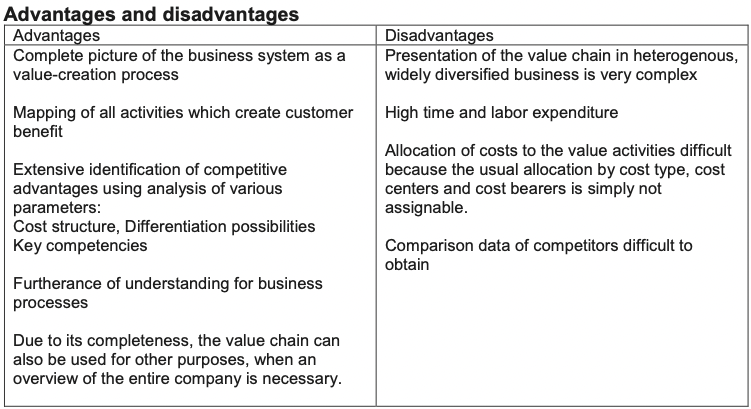
\includegraphics[width=9cm]{Images/Value Creation - Pros and Cons.png}
\end{center}
\newpage
\section{General Aviation}
\underline{\textbf{Definition and Scope} - ICAO see slide 6}
\begin{itemize}
    \item Flight School
    \item Law enforcement 
    \item Firefighting
    \item Sightseeing
    \item Package Delivery 
    \item Air Ambulance 
    \item News/traffic reporting 
    \item Agriculture 
    \item Wildlife Management 
    \item Recreational Flying 
    \item Disaster Relief 
    \item Mountain Support 
\end{itemize}
\underline{\textbf{Modes of Transport}}
\begin{itemize}
    \item Powered Flight 
    \item Gliding
    \item Skydiving
    \item Helicopter
    \item Ballooning 
    \item Not in GA: Scheduled line flight, Commercial Business Jet FLight, Charter Flight, Military Flight
\end{itemize}
\underline{\textbf{Interest Groups/Associations}}
\begin{itemize}
    \item Aero-Club Switzerland (AeCS): represents 24,000 members in the field of light aviation \& aerial sports
    \item Aircraft Owner and Pilots Association: represent the interests of private pilots and aircraft owners (3500 members) in national and international aviation committees.
    \item Aero Suisse: (political organisation) safeguarding the interests of civil aviation and space travel in Switzerland and securing their basic existence. It has an influence on the design of the legal principles in the field of aerospace (150 companies)
\end{itemize}
\underline{\textbf{General Aviation - Numbers}}
\begin{itemize}
    \item Worldwide:
    \begin{itemize}
        \item 1.1 Million pilots (2018) (2015/700K)
        \item 340'000 A/C (370'000)
        \item 35 Million FH (40)
        \item Value Creation 40 Billion USD (comparison)
        \item Comparison to CAT (Commercial Air Transport): 60'000 A/C / 400'000 Pilots
    \end{itemize}
    \item CH:
    \begin{itemize}
        \item 3 National Airports: 450k Movements per year 
        \item 11 Regional Airports: included above
        \item 47 Airfields: 500k Movements 
        \item 24 Heliports
        \item 500'000 PAX transported (1\% of all PAX: Swiss Intl. 16 Million)
        \item 270'000 Tonnes freight 
    \end{itemize}
    \item Value Creation 
    \begin{itemize}
        \item 500 Million CHF
        \item Turnover: 1 Billion CHF
    \end{itemize}
\end{itemize}
\underline{\textbf{Divisions}}
\begin{itemize}
    \item Powered Flight 
    \item Gliding 
    \item Skydiving/parachute jumping  
    \item Helicopters
    \item Balloons 
    \item Ecolight
    \item Experimental
\end{itemize}
\underline{\textbf{Powered Flight}}
\begin{itemize}
    \item Single Engine Piston (SEP): Examples - Cessna 172 Skyhawk, Piper PA-28-161-Warrior
    \item License Extensions
    \begin{itemize}
        \item Towing of gliders
        \item Aerobatics: Minimum flight altitudes of 500m above
        ground or 300m for glider pilots. Aerobatics over densely populated areas and airfields is prohibited.
        With special training you can go down to 100m for competitions.
    \end{itemize}
    \item Mountain Flight/Glacier landings (MOU)
        \begin{itemize}
            \item In Switzerland there are 40 designated glacier airfields at over 1100m above sea level.
            Glacier flights are challenging because of the reduced engine power required to operate in a harsh environment and the changing “runways".
        \end{itemize}
    \item Seaplanes 
    \begin{itemize}
        \item Float plane flying is restricted in Switzerland, but there are exception permits for events such as the Fly-In in Hergiswil.
        Many Swiss pilots go to Como or Canada to get their licenses.
    \end{itemize} 
    \item Precision Flights (Powered Flights competition)
    \begin{itemize}
        \item Theory: flight preparation: this is about exactly calculating a flight over five to eight legs, with a given wind, under time pressure (maximum 30 minutes).
        \item Nav-flight: The prepared route (length 170 to 260 km) is now flown to the nearest second and meter.
        \item Precision landings: 4 precision landings in different configurations (with and without power) complete the competition programme, whereby it is important to place the main landing gear as cleanly as possible on the zero line.
    \end{itemize}   
\end{itemize}
\underline{\textbf{Gliding}}
\begin{itemize}
    \item Aspects of Gliding
    \begin{itemize}
        \item Comradship (working as a team)
        \item Learn to fly at low cost (6-7000 CHF)
        \item High Performance Sport (Alone in cockpit for few hours), make important decisions at high altitude with constant sun radiation 
        \item Learn precise flying: Gliding is about optimization in order to stay in the air as long as possible. Gliders can reach a glide ration of 80
    \end{itemize}
    \item Operations (Sources of Energy)
    \begin{itemize}
        \item Slope winds on the LUV side 
        \item Using thermals underneath the clouds (cumulus), heights up to 5000m can be reached (to the upper cloud limits is possible)
        \item Wave flight: LEE waves occur in particular strong conditions on the windless side of the mountain (Lenticularis Cloud). 8000m can be reached this way (oxygen, pressure suits and thermal clothing needed) 
    \end{itemize}
    \item Cloud flights and competitions 
    \begin{itemize}
        \item Specially established gliding zones with reduced cloud distance of
        100m horizontal and 50m vertical
        \item in order to make full use of the thermals, there is a so-called cloud flight, analogous to flying with instruments.
        The competition is limited to aerobatics and large distance flights.
    \end{itemize}
\end{itemize}
\underline{\textbf{Skydiving / Parachute Jumping}}
\begin{itemize}
    \item Procedure 
    \begin{itemize}
        \item Air drop machine (Pilatus Porter, Cessna 182 or 206)
        \item Classical Jump from 3500-4000m above sea-level 
        \item Freefall at 200km/h (belly-first) and 360km/h head-first 
        \item 50 sec freefall 
        \item Release of parachute at 700-800m above ground, latest at 400 m (automatic emergency opening due to height and drop rate at 250m)
        \item Round canopy or paraglider 
        \item Paraglider 60km/h forward speed and 5m/s drop rate 
    \end{itemize}
    \item Military Variations 
    \begin{itemize}
        \item HALO (High Altitude Low Opening): 8000m height and late opening (800m)
        \item HAHO (High ALtitude High Opening): Long glide flight used ($>40km$)
        \item Can be tried also by civilians 
    \end{itemize}
    \item Competition 
    \begin{itemize}
        \item Target jumping: Landing on an electronic target as accurately as possible 
        \item Freestyle Jumping: Completing figures
        \item Formation or relative jumping: Formation of colleagues form as many as pre-defined figures as possible
    \end{itemize}
\end{itemize}
\underline{\textbf{Helicopter}}
\begin{itemize}
    \item Differences in OPS 
    \begin{itemize}
        \item Can stay still without moving forwards 
        \item Parag. 38 VVR: Helicopters can fly with a visibility of less than 1,5 km if they move with a flight speed that allows them to recognize other aircraft or obstacles in good time to avoid collisions. Below 1100m above sea level helicopters, for the most part, do not have to fly from an airfield (external landing provision)
        \item Helis are only fully IFR-compatible in the higher weight classes ($>$3.5t)
        \item No starting or landing runways are required (twice rotor diameter sufficient)
        \item No pressurised cabin: Max altitude 6000m (exceptions up to 7000m)    
    \end{itemize}
    \item Range of Operations 
    \begin{itemize}
        \item Transport of materials 
        \item External Cargo Sling (ECS): ECS 1: $\leq$20m /ECS 2: $>$20m/ ECS 3: Logging
        ECS 4: Construction /HCS: Human Cargo Sling
        \item Transport of people 
        \item Dropping off parachute jumpers 
        \item Measuring, photography/films, control flights 
        \item Avalanche triggering 
        \item Mountain hut supplies 
        \item Animal transport 
        \item Corporate Flights (inhouse company transports, goods, own personnel)
        \item Rescue Flights
        \begin{itemize}
            \item Primary Missions: Direct flights from scene of accident to medical centre 
            \item Secondary Missions: Relocation of patients from hospital to hospital 
        \end{itemize}
        \item On behalf of authorities and civil organisations or scheduled flights (overseas, to oil platforms ATPL(H))
        \end{itemize}
        \item Classical Types: Ecureuil AS 350 B3, Kamov KA 32 A12 
        \item Critical voices: 
        \begin{itemize}
            \item A lot of media coverage compared to share of GA (5-10\%)
            \item Noise at low operating levels is a big topic of discussion 
            \item Heli-skiing a strong polariser, however offers cheap opportunities for training/learning flights
        \end{itemize} 
\end{itemize}
\underline{\textbf{Balloons}}
\begin{itemize}
    \item Types of Balloons: Gas balloon (hydrogen), hot-air ballon (warm air)
    \begin{itemize}
        \item Balloons travel, because they ride with the wind (therefore always windstill in basket)
        \item Balloons do not like thermals, therefore flights are performed in the mornings and evenings (ideally winter)
        \item 350 licenses currently issued for 380 balloons 
        \item Switzerland has the highest density of balloons in the world 
        \item Balloons cost up to 100k CHF, therefore mostly company sponsored (advertising) or are owned by clubs (gas balloons)
    \end{itemize}
   \item Operations of Gas Balloons
   \begin{itemize}
       \item Control by making use of winds 
       \item Climb rate max 9m/s (normally 3-4m/s)
       \item Max. Capacity 12 people 
       \item Gas balloon 
       \begin{itemize}
           \item Ideally helium (safe, and high climb rate, but too expensive, therefore hydrogen)
           \item Quiet (no burner)
           \item Needs filling station (in CH only in Zurzach)
           \item Is up to 100h in the air 
           \item Load-bearing capacity: 1$kg/m^3$
           \item One filling: 2000 CHF (more expensive)
           \item Height Control: Release sand (climb), or gas (descend)
       \end{itemize}
       \item Hot Air Balloon 
       \begin{itemize}
           \item Up to 4 burners (only 1 in use): propane gas bottles (30-40 kg / 4 units)
           \item Up to 15h in air 
           \item With 4 bottles normally 2-3 hours 
           \item For competitions: 5-6 hours 
           \item Load-bearing capacity: 250$g/m^3$
           \item Height control: with burner 
           \item Temperature in balloon: 80-100$^\circ$ C 
       \end{itemize}
       \item Competitions
       \begin{itemize}
           \item Navigation trips, in which waypoints or targets must be approached or overflown 
           \item Long-distance trips 
       \end{itemize}
   \end{itemize}
\end{itemize}
\underline{\textbf{Ecolight}}: Since 4.7.2011, Light Sport Aircraft (LSA 600) have been allowed in Switzerland (up to 600kg); however, Ecolights/ Ultralights under 427.5 kg were banned. As of 1.10.2014, these have also been allowed (electr. UL without landing gear remain banned).
\newpage
\section{Aircraft Design \& Systems}
\underline{\textbf{Definitions}}
\begin{itemize}
    \item \textbf{System}: A combination of parts, components, facilities, procedures, personnel, skills, ... that are connected in an organized way to perform one or more functions
    \item \textbf{Function}: The lowest level of a specific action of a system, equipment, and flight crew performance on the airplane
    \item \textbf{Failure}: The inability of a system, subsystem or component to perform a function as intended (Functional Failure)
    \item \textbf{Failure Condition (FC)}: A condition with an effect on the aircraft and its occupants caused by one or more failures considering the relevant operational and environmental conditions
\end{itemize}
\begin{center}
    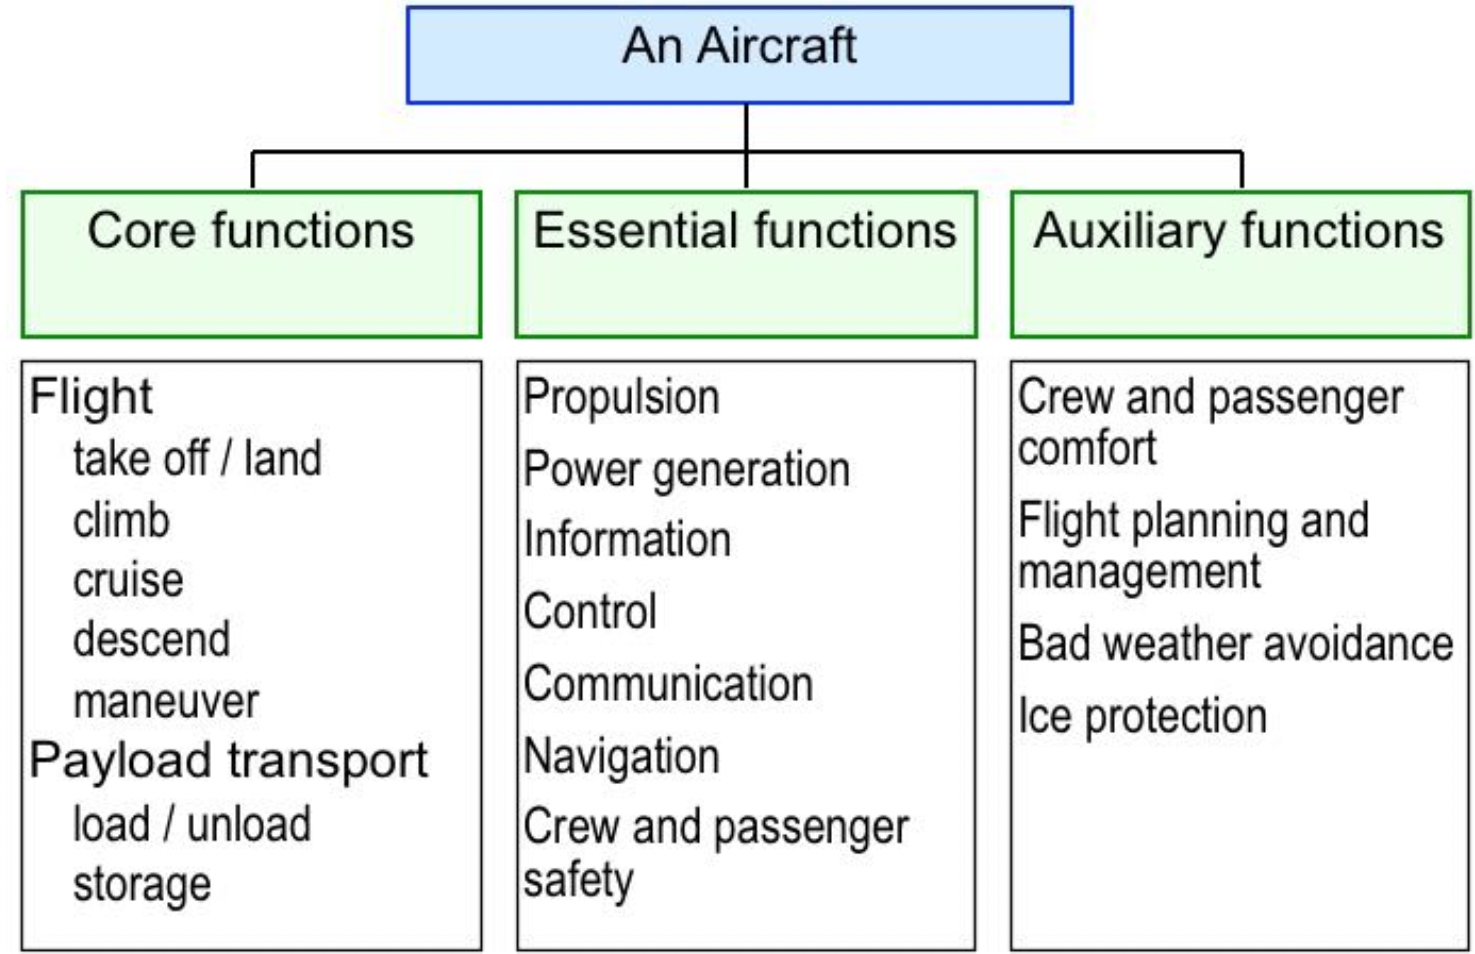
\includegraphics[width=9cm]{Images/Systemisation-Aircraft-Function.png}
    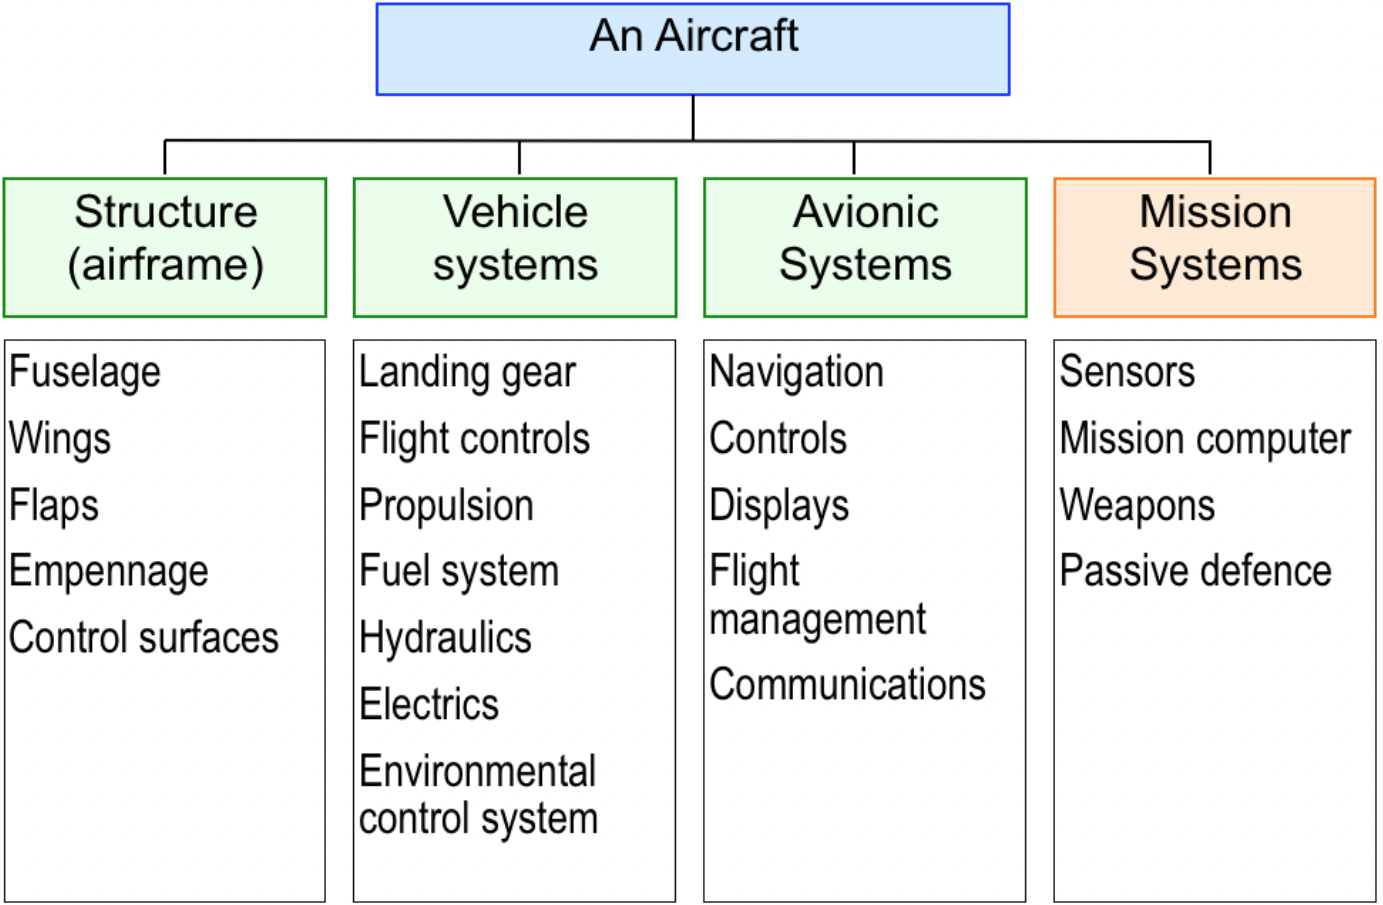
\includegraphics[width=9cm]{Images/Systemisation-Aircraft-System.png}
\end{center}
Example:
\begin{itemize}
    \item \textbf{System}: Navigation and Spatial Orientation (Avionics System)
    \item \textbf{Function}: Display current altitude 
    \item \textbf{Failures}: Loss of Altitude Indication. Misleading Altitude Information 
    \item \textbf{Failure Conditions}: Loss of ALT - VMC - All Flight Phases or Misleading ALT Indication - IMC - Approach/Landing 
\end{itemize}
\underline{\textbf{Failure Condition Classification}}
\begin{itemize}
    \item \textbf{Minor (D)}: No significant reduction in airplane safety, corrective actions well within crew capability, physical discomfort to passengers or cabin crew (Safety objectives not required)
    \item \textbf{Major (C)}: Significant reduction of safety margin, increase in crew workload, physical distress to crew or occupants, possibly including injury (May be required)
    \item \textbf{Hazardous (B)}: Large reduction of safety margin, physical distress or large increase in crew workload, serious or fatal injury to occupants (May be required)
    \item \textbf{Catastrophic (A)}: Multiple fatalities of the occupants, serious or fatal injury to flight crew members, loss of aircraft (Required)
\end{itemize}
\underline{\textbf{Failure Condition Probability}}
\begin{itemize}
    \item \textbf{Probable} failure conditions are those anticipated to occur one or more times during the entire operational life of each airplane
    \item \textbf{Remote} failure conditions are those unlikely to occur to each airplane during its total life but which may occur several times when considering the total operational life of a number of airplanes of this type
    \item \textbf{Extremely Remote} failure conditions are those not anticipated to occur to each airplane during its total life but which may occur a few times when considering the total operational life of all airplanes of this type
    \item \textbf{Extremely Improbable} failure conditions are those so unlikely that they are not anticipated to occur during the entire operational life of all airplanes of one type
\end{itemize}
\underline{\textbf{Acceptable Probabilites for commuter or transport A/C}}
\begin{itemize}
    \item Probable corresponds to a probability lower than $10^{-3}$ but higher than $10^{-5}$
    \item Remote corresponds to a probability lower than $10^{-5}$ but higher than $10^{-7}$
    \item Extremely remote corresponds to a probability lower than $10^{-7}$ but higher than $10^{-9}$
    \item Extremely Improbable corresponds to a probability lower than $10^{-9}$ (light general aviation: $10^{-6}$)
\end{itemize}
\underline{\textbf{Design Concepts}}
\begin{itemize}
    \item \textbf{Safe-Life}: systems or components will survive a specific design life with no failures
    \item \textbf{Fail-Safe}: a failure will cause no (or minimum) harm to other parts and systems or danger to
    personnel
    \item \textbf{Fault-Tolerant}: a system can continue operating in the event of the failure of one or more of its components
\end{itemize}
\underline{\textbf{Examples of Design Concetps}}
\begin{itemize}
    \item Safe-Life: the emergency oxygen system in an airliner. The chemical cartridges that generate oxygen have a prescribed life and must be replaced after a certain period. The manufacturer guarantees that the cartridges will not fail (meaning, in practice, that a failure is extremely improbable) during their life span.
    \item Fail-Safe: In air brakes on railway trains (Westinghouse system), the brakes are kept open by air pressure in the brake system. Should a brake line split, or a carriage become de-coupled, the air pressure will be lost and the brakes applied. The system is designed to avoid dangerous situations for people and material, and as such it can be defined Fail-Safe. Other example: Landing Gear of Pilatus PC-12
    \begin{itemize}
        \item In any system or subsystem, the failure of any single element, component, or connection during any one flight (brake release through ground deceleration to stop) should be assumed, regardless of its probability. Such single failures should not prevent continued safe flight and landing, or significantly reduce the capability of the airplane or the ability of the crew to cope with the resulting failure conditions.
        \item Subsequent failures during the same flight, whether detected or latent, and combinations thereof, should also be assumed, unless their joint probability with the first failure is shown to be extremely improbable.
    \end{itemize}
    \item Fault-tolerant: Fly-by wire system (also Fail-safe)
\end{itemize}
\underline{\textbf{Safety Processes}}
\begin{enumerate}
    \item Hazard Identification (List of possible failures)
    \item Risk Assessment (consequences)
    \item Acceptable? 
    \item If NO, Risk Mitigation Method and do another Risk Assessment. If YES, done 
\end{enumerate}
\underline{\textbf{Safety Processes - Example of Safety Requirements}}
\begin{itemize}
    \item The average probability per flight hour of loss of all means of altitude information shall be less than $10^{-9}$
    \item There shall be no single failure resulting in loss of all means of attitude information 
\end{itemize}
\underline{\textbf{Summary of basic principles (see script)}}
\begin{itemize}
    \item Distinguish hazards from failures is essential to understand the difference between safety and reliability
    \item The criticality of failure conditions, not the criticality of faulty components, determines the level of analysis required 
    \item A safety process at the END of development is useless 
    \item The successful safety process is INTEGRAL to development 
    \item In future, the safety process will GUIDE development
\end{itemize}
\underline{\textbf{Failure Hazard Analysis (FHA)}} \\ \\ 
A FHA is carried out at both aircraft and system levels; one flows down from the other. The FHA identifies functional failure conditions and determines their effects. The FHA identifies the failure conditions and their effects on aircraft and crew. These allow to define the safety objectives and a quantitative probability requirement for that particular condition. \\ \\ 
\underline{\textbf{Preliminary System Safety Analysis (PSSA)}} \\ \\ 
The PSSA examines the failure conditions established by the FHA(s) and demonstrates how the system design will meet the specified requirements. Various techniques (such as FTA, Fault Tree Analysis) may be used to identify how the design counters the effects of various failures and may point towards design strategies which need to be incorporated in the system design to meet the safety requirements. Typical analyses may include the identification of system redundancy requirements, e.g. how many channels, what control strategies could be employed and the need for dissimilarity of control, for example dissimilar hardware or dissimilar software implementations, or both. The PSSA is therefore part of an iterative process which scrutinises the system design and assists the system designers in ascribing and meeting risk budgets across one or a number of systems. \\ \\ 
\underline{\textbf{System Safety Analysis (SSA)}} \\ \\ 
The SSA is a systematic and comprehensive evaluation of the system design using similar tech- niques to those employed during the PSSA activities. However, whereas the PSSA identifies the requirements, the SSA is intended to verify the that the proposed design does in fact meet the spec- ified requirements as identified during the FHA and PSSA analyses conducted previously. The SSA occurs at the point in the design cycle where the system implementation is concluded or finalised, and prior to system certification. \\ \\ 
\underline{\textbf{Common Cause Analysis (CCA)}} \\ \\ 
The CCA begins concurrently with the system FHA; it interacts with this activity and with sub- sequent PSSA and SSA analyses. The purpose of the CCA is, as the name suggests, to identify common cause or common mode failures in the proposed design and assist the designers to develop strategies which will make such failures impossible. Such common cause failures may include:
\begin{itemize}
    \item Failure to correctly identify the requirement
    \item Failure to correctly specify the system
    \item Hardware design errors
    \item Component failures
    \item Software design and implementation errors
    \item Software tool deficiencies
    \item Maintenance errors
    \item Operational errors
\end{itemize}
The CCA is therefore intended to scrutinise a far wider range of issues than the system hardware or software process. Rather it is meant to embrace the whole process of developing, certifying, operating and maintaining the system throughout the life cycle. \\ \\ 
\underline{\textbf{Component Reliability}}
In system safety analysis, a great deal of emphasis is placed upon the failure rate of a component or element within the system under review. This clearly calls into question how reliability values for different type of component are established. There are two main methods of determining component reliability:
\begin{itemize}
    \item Analytical by component count (issues)
    \begin{itemize}
        \item only as good as the data base of components and the factors used
        \item predicted values are generally pessimistic thereby generating predicted failure rates worse than might be expected in real life
        \item the technique has merit in comparing competing design options in a quantitative manner when using a common baseline for each design (good)
        \item it is difficult to continue to update the data base; particularly with the growing levels of integration with Integrated Circuits (ICs)
        \item increasing number of Commercial Off-The-Shelf (COTS) components also confuses the comparison
        \item technique is particularly valuable when it can be compared with in-service experience and appropriate correction factors applied (good)
    \end{itemize}
    \item Historical by means of accumulated in-service experience
    \begin{itemize}
        \item 
    \end{itemize}
\end{itemize}
\underline{\textbf{Maintenance Concepts}}
\begin{itemize}
    \item Corrective maintenance: Refers to the repair or replacement of components, parts or subsys- tems which have failed or broken down
    \item Periodic maintenance: Refers to the scheduled overhaul or replacement of parts (Hard-Time) or to scheduled checks and inspections of parts to remove them from service before a failure can occur (On-Condition)
    \item Predictive maintenance: Refers to the monitoring of relevant operating parameters in a part or in a system to predict an incoming failure (Condition-Monitoring)
\end{itemize}
\newpage
\section{Airport Planning}
\underline{\textbf{Swiss Airport Landscape}}
\begin{itemize}
    \item 31 Million ZRH 
    \item 15.5 M GVA 
    \item 10 Million BSL 
\end{itemize}
\underline{\textbf{Europe}}
\begin{itemize}
    \item Europe Airport Landscape: Movements vs Passenger is different (shows there are differences in efficiency)
    \item Movement = 1 Takeoff or Landing 
    \item Connectivity in Europe: Connecting destinations + frequency of flights to the same destination (density)
\end{itemize}
\underline{\textbf{Worldwide}}
\begin{itemize}
    \item Hub connectivity (Airport connectivity = sum of direct and indirect connectivity to the rest of the world through direct flights or indirect connections)
    \item Even though there are larger airports with more passengers around the world, European Airports are more connected
    \item Lenght of runways has a large impact. PC24 can land quite on very short runways 
\end{itemize}
\underline{Examples}
\begin{itemize}
    \item Male: Passengers distributed by water planes or boats + Large A/C on runways 
    \item Sao Paulo Congonhas: Sever traffic needs (Sao Paulo to Rio) + 2 RWY up to code C + private jets. Not compliant today
    \item Hongkong: Built on island (based on sketch). Only runway and terminal (Y-Footprint for efficiency)
    \item Amsterdam: Developed over 100 years (historically)
    \item Atlanta: Many runways, linear structures hence high capacity 
    \item Istanbul: Y-Footprint, based off sketch 
\end{itemize}
\underline{\textbf{User- and stakeholder requirements}}
\begin{itemize}
    \item Historically: Military + Government, today: Mixed ownership 
    \item Passengers: Simplified Procedures
    \item Airlines: Customer Satisfaction 
    \item Technology Vendors: Solution Providers 
    \item Airports: Better resource use 
    \item Border Agencies: Improved controls 
\end{itemize}
\underline{\textbf{Traffic Analysis - Main parameters}}
\begin{itemize}
    \item Flight Schedule 
    \item Number of air passengers (terminal capacity)
    \item Number of flight movements (runway, apron and airspace capacity)
    \item Cargo tonnage (size of cargo facilities)
    \item Traffic pattern (scheduled/charter/general aviation/military/IFR/VFR/training)
    \item Destinations (Schengen/non-Schengen, EU/International)
    \item Fleet mix (Design Aircraft, Airfield Layout, size and mix of aircraft stands)
    \item Number of parked Aircraft (Number of Aircraft Stands and Hangar Space)
    \item Airline Mix (Terminal Layout)
    \item Yearly traffic pattern, weekly traffic pattern, daily traffic pattern (peak hours, relevant intervals for facility sizing)
\end{itemize}
\underline{\textbf{Numbers}}
\begin{itemize}
    \item Ratio passengers vs. A/C movements: Correlated and proportional
    \item Ratio passengers/movement vs passengers/year: Correlated and proportional 
\end{itemize}
\underline{\textbf{Traffic Forecast}}
\begin{itemize}
    \item Different sources, see slide 38
\end{itemize}
\underline{\textbf{Design Parameters}}
\begin{itemize}
    \item A/C movements per year or hour 
    \item Passenger per year, hour and transfer ratio 
    \item Cargo tonnage per year
    \item Design aircraft
    \begin{itemize}
        \item Wingaspan Code F: 65-80 m (B777, and possible to fold wings to change from E on aprons to F on runway)
        \item E: 52-65 m 
        \item D: 36-52m
        \item C: 24-36m (A320)
    \end{itemize}
\end{itemize}
\underline{\textbf{Main airport logistics flows}}
\begin{itemize}
    \item A/C guidance (On block to off block)
    \item A/C handling (deboarding to boarding)
    \item Bag handling (unloading + bag claim to loading + check in)
    \item Pax handling (boarding to deboarding))
\end{itemize}
\underline{\textbf{Laws and Standards}}
\begin{itemize}
    \item ICAO: Public international law (Annex 14 Aerodromes)
    \item EASA: Adapts ICAO into European context (FAA for US) - EASA CS-ADR-DSN
    \item Countries define national standards (often adapted from ICAO or EASA)
    \item IATA delivers guidance 
    \item Switzerland: Federal laws, + spatial planning law (SAIP), Aviation Law, Environmental Law, Conservation Law
\end{itemize}
\underline{\textbf{Site Analysis and Boundary Conditions}}
\begin{itemize}
    \item Airspace (availability due to other airports etc.)
    \item Topography (consider mountains etc. as small approach angles $3^\circ$)
    \item Meteorology: Wind (against landing and takoff), visibility, Temperature 
    \item Space Requirements (some dense)
    \item Geology, storms, water, fauna 
    \item Location related to city (80\% close to city center = 15km), also attracts settlement and industry 
    \item Public Infrastructure (Airport equals midsize city, redundant power supply, water supply, waste disposal, fuel delivery)
    \item Noise (take-off=wide area due to more noise during liftoff)
\end{itemize}
\underline{\textbf{Airport Elements}}
\begin{itemize}
    \item Runway System
    \begin{enumerate}
        \item Runway with turnpads (length typically 4km)
        \item Parallel taxiway (shorter sequences Takeoff and Landing)
        \item Rapid exits 
        \item Multiple entries 
        \item 2nd parallel taxiway 
        \item 2nd runway
    \end{enumerate}
    \item Obstacle limitation 
    \item Apron and taxiway system (depend on)
    \begin{itemize}
        \item Fleet mix 
        \item Number of A/C in peak hour 
        \item Number of A/C overnight 
        \item Rule of thumb: Stands $\approx$ 1.25 runway capacity/hour 
        \item 1 stand wingspan code E = $10'000~m^2$ concrete (1 hectar)
        \item Code C= $5'000~m^2$
        \item Requires enough space for different vehicles to deliver fuel, supplies etc.
    \end{itemize}
    \item Terminal Footprints
    \begin{itemize}
        \item Linear structures will yield shorter distances to walk 
        \item Terminal Sections: Multiple levels for separation of inbound and outbound PAX 
    \end{itemize}
    \item Baggage handling, performance measured by 
    \begin{itemize}
        \item Capacity/hour 
        \item Security Requirements 
        \item Customs Requirements 
        \item Transfer Share 
        \item Minimum Connecting Time 
        \item Self handling vs. multi airline ground handling 
    \end{itemize}
    \item Landside Access (parameters)
    \begin{itemize}
        \item Taxi, public bus vs self-driven vehicles $\rightarrow$ curbside, parking 
        \item Road vs. rail 
        \item Segregated flows for people and goods 
    \end{itemize}
    \item Landside commercial utilization (airport city)
    \begin{itemize}
        \item Well frequented sites are attractive for real estate development 
        \item Additional source of income for airport operators 
    \end{itemize}
    \item Cargo 
    \item Aircraft Maintenance 
    \begin{itemize}
        \item Admin 
        \item Airport Maintenance 
        \item Workshops 
        \item Fire fighting \& rescue 
        \item Fuel farm 
        \item Airline facilities 
        \item Meteo 
    \end{itemize}
\end{itemize}
\underline{\textbf{Rules of thumb}}
\begin{itemize}
    \item Simple runway: 10-20 movements per hour 
    \item Runway with taxiway and rapid exits: 40-50 movements per hour 
    \item Parallel runway system: 90-12 mvmts/hour, $10-15~km^2$
    \item Number of stands $\approx$ 1.25 RWY capacity/hour
    \item 2.75 stands per 1 Million Pax / Year 
    \item Wingspan Code E = 10'000 $m^2$ concrete 
    \item 10'000 $m^2$ terminal space $\approx$ 1 Million PAX/year 
    \item 50-150 PAX/Mvmt 
    \item 1M PAX/Year $\approx$ 1000 staff 
    \item Traffic Growth $\approx$ 2 x GDP growth (in country)
\end{itemize}
\underline{\textbf{Economical Aspcects}}
\begin{itemize}
    \item Aviation Revenue + Non-Aviation Revenue: Both are highly important to break even or make profit 
\end{itemize}
\newpage 
\section{Airport Operations}
\begin{itemize}
    \item Aircraft Operations
    \item Landside Operations (Terminal)
    \item Billing and Invoicing 
    \item Information Management 
\end{itemize}
\subsubsection{Aircraft Operations}
\begin{itemize}
    \item Ground Handling 
    \begin{itemize}
        \item Passengers: Boarding/Deboarding + Transport 
        \item Baggage: Loading/Unloading + Transport 
        \item Cargo: Loading/Unloading + Transport 
    \end{itemize}
    \item Aircraft Services 
    \begin{itemize}
        \item Catering 
        \item Cleaning 
        \item Waster/Waste 
        \item Fuel 
        \item De-icing 
        \item Line Maintenance 
    \end{itemize}
    \item Apron Maintenance Service 
    \begin{itemize}
        \item Aircraft Guidance: Apron Control, Follow-me, Marshalling 
        \item Aircraft Stand Allocation 
        \item Aircraft Push-back 
    \end{itemize}
    \item Safety
    \begin{itemize}
        \item Obstacle Management 
        \item Wildlife Management 
        \item Runway \& Surface Inspection 
        \item Runway \& Surface Maintenance 
        \item Snow Removal 
    \end{itemize} 
\end{itemize}
\underline{\textbf{Regulatory Framework for Airport Operations}}
\begin{itemize}
    \item Concession Agreement 
    \begin{itemize}
        \item Authorises and commits a company to operate an airport 
        \item Regulates financing and charging 
        \item Issued by the federal or regional government 
        \item Varies widely in scope and detail 
        \item Several concessions possible for particular activities 
    \end{itemize}
\end{itemize}
\underline{\textbf{National Authority}}
\begin{itemize}
    \item ICAO SARPS to be implemented by national authority 
    \item FOCA 
    \begin{itemize}
        \item Responsible for monitoring civil aviation in Switzerland and aviation development
        \item Ensuring that civil aviation in Switzerland has a high safety standard and one that it is in keeping with sustainable development
        \item Supervises aviation companies to which it issues an operating licence based on a technical, operational and financial evaluation
    \end{itemize}
\end{itemize}
\underline{\textbf{Accountable Airport Manager}}
\begin{itemize}
    \item In CH: Organised through the Aviation Infrastructure Ordinance 
    \item Commission Regulation (EU) 139/2014
    \item The aerodrome operator shall appoint an accountable manager, who has the authority for ensuring that all activities can be financed and carried out in accordance with the applicable requirements. The accountable manager shall be responsible for establishing and maintaining an effective management system.
\end{itemize}
\underline{\textbf{Runway Capacity Allocation: Slot Coordination}}
\begin{itemize}
    \item Mission: 
    \begin{itemize}
        \item Allocation of constrained or limited airport capacity to airlines and other A/C operators 
        \item Maximise the efficient use of airport infrastructure 
        \item Maximise the benefits to the greatest number of airport users 
    \end{itemize}
    \item Organisation:
    \begin{itemize}
        \item Slot Coordination Switzerland
        \item Independent Non-Profit Organisation
        \item Regulation EEC95/93
        \item Federal decree for seasonal airport slot planning and allocation 
    \end{itemize}
\end{itemize}
\subsubsection{Landside Operations (Terminal)}
\begin{itemize}
    \item Terminal
    \begin{itemize}
        \item Passengers: Checkin/Bag drop, Security Check, Passport Control (immigration/emigration), Transport, Boarding 
        \item Baggage: Bag drop, Transport, Security Check, Sorting, Delivery  
    \end{itemize} 
    \item Others
    \begin{itemize}
        \item Cargo: Truck loading/unloading, Storage, Packaging/Re-packaging, Security Check 
        \item Customs: All areas 
        \item Police: All areas 
    \end{itemize}
    \item Access 
    \begin{itemize}
        \item Car Parking 
        \item Drop-off / Pick-up 
        \item Bus Station 
        \item Railway Station 
        \item Taxi Stand 
        \item Truck Ramp 
    \end{itemize}
\end{itemize}
\subsubsection{Billing and Invoicing - see Slide 37}
\subsubsection{Information Management}
\begin{itemize}
    \item Airport Operational Database 
    \begin{itemize}
        \item Core IT system for airport operations
        \item Storage, processing and provision of flight and passenger related data
        \item Basis for Billing
    \end{itemize}
    \item Data Examples 
    \begin{itemize}
        \item Airline Schedules
        \item Daily Flight Plans
        \item Gate allocation
        \item A-CDM Time-stamps
        \item Nr. of Passengers, Transfer
        \item Nr. of Baggage 
    \end{itemize}
\end{itemize}
\subsubsection{Zurich Flughafen AG}
\begin{itemize}
    \item 280 Companies, 27'000 Jobs 
    \item 31.5 Mio PAX per year, 86'000 per day 
    \item Transfer passengers: 29.3\% 
    \item 275'000 Flights per year, 750 per day 
    \item Peak day: 907 flights, 115'000 PAX 
    \item 203 destinations, 77 airlines 
    \item Federal Mandate: DETEC concession agreement 2001-2051
    \item Public Company: Shareholders: Public trading 61.7\%, Canton of Zurich 33.3\%, City of Zurich 5\%, Not subsidised 
    \item Flughafen ZRH AG (2019): 1.2 Billion turnover, 309.1 Million revenue, 1700 employees, 4.59 Million Balance sheet total 
    \item Projects around the world, mostly in South America (Brazil, Colombia, Chile), some also in India  
\end{itemize}
\subsubsection{Challenges to Airport Operations}
\begin{itemize}
    \item Aircraft Turn-around 
    \begin{itemize}
        \item Turnaround Process 
        \item Collaborative Decision Making (A-CDM)
        \item Departure Management 
    \end{itemize}
    \item Airport operations plan 
    \item Adverse Conditions 
    \item Hub Operation 
\end{itemize}
\underline{\textbf{Aircraft Turn-around}}
\begin{itemize}
    \item Starts with On block step until Pushback of the vehicle 
    \item Service Providers Included 
    \begin{itemize}
        \item Gound Handling Company 
        \item Airport Operator 
        \item Airline 
        \item ATC 
        \item Fuel Service 
        \item Catering 
        \item Cleaning 
        \item Waste Water 
        \item Freight Forwarder 
        \item Aircraft Maintenance 
        \item Police 
    \end{itemize}
    \item Indispensible services provided by third parties 
    \item No or only general contractual relationship between airport operator and service provider, i.e.
    \begin{itemize}
        \item Skyguide: Legal mandate issued by Swiss Confederation
        \item Police: Sovereign state duty 
        \item Handling agents: Contracts with airlines 
    \end{itemize}
    \item \textbf{Performance-relevant processes are not under managerial control of airport operator}
\end{itemize}
\underline{\textbf{Collaborative Decision Making}}
\begin{itemize}
    \item Developed and supported by Eurocontrol
    \item Implementation required at all major airports in Europe 
    \item Defines processes for airport operations: Rules and procedures, Input and output information requirements, Human-Machine-Interface (HMI) requirements 
    \item A-CDM requires platform (to include ATC, Airline Operator, Network Manager, Airport Operator, Ground Handling)
\end{itemize}
\underline{\textbf{Departure Management System}}
\begin{enumerate}
    \item System calculates optimum take-off sequence, based on 
    \begin{itemize}
        \item ATC flight plan 
        \item ATC slot 
        \item RWY concept 
        \item Aircraft wake turbulence category
        \item Aircraft speed class 
        \item Departure route 
    \end{itemize}
    \item Result: Calculated Take-Off Time (CTOT) for each flight 
    \item Calculation of Target Start-up Approval Time (TSAT)
    \begin{itemize}
        \item Consideration of taxi time from stand to RWY 
        \item Considering Target Off-Block Time (TOBT)
    \end{itemize} 
\end{enumerate}
\underline{\textbf{Time Stamps}}
\begin{itemize}
    \item Target Off-Block Time (TOBT) (must be ready within +- 5min of official TBOT to push back)
    \begin{itemize}
        \item The time that the Aircraft Operator or Ground Handler estimates that an A/C is ready, all doors closed, boarding bridge removed, push back vehicle available and ready to start up / push back immediately upon reception of clearance from the Tower 
    \end{itemize}
    \item Target Start-Up Approval Time (TSAT) (created 30 min before TBOT)
    \begin{itemize}
        \item Provided by ATC, taking into account TOBT, CTOT and/or the traffic situation that an aircraft can expect start-up/push-back approval 
    \end{itemize}
    \item Calculated Take-Off Time (CTOT)
    \begin{itemize}
        \item A time calculated and issued by the appropriate Central Management unit, as a result of tactical slot allocation, at which the flight is expected to be airborne 
    \end{itemize}
\end{itemize}
\underline{\textbf{Airport Operations Plan}}
\begin{itemize}
    \item Timeline: 3 hours to 180 days with decreasing precision vs. A-CDM time-line approx 3h
    \item Predictability: Continuously updated plan of airport operations, and includes all relevant infos (pax, baggage, A/C, ATC)
    \item Common picture for all stakeholders: Information sharing 
    \item Essential to increase efficiency of airport operations: Prerequisite for arrival steering
\end{itemize}
\underline{\textbf{Arrival Steering - Target Time of Arrival (TTA)}}
\begin{itemize}
    \item Today: Regulated by Eurocontrol only (no ATC etc.) to meet capacity limits. Overdemand is delayed at departure airport to avoid airborne holding
    \item TTA Concept: Airport, ATC and Airline define together optimal sequence of arriving traffic, and gets it reviewed by Eurocontrol. Eurocontrol delays flights of departures accordingly
\end{itemize}
\underline{\textbf{Adverse Conditions}}
\begin{itemize}
    \item Strong Winds
    \item Thunderstorms 
    \item Snow 
    \item Winter 
    \item Fog 
\end{itemize}
\underline{Strong Winds}
\begin{itemize}
    \item Impact on Flight Operations
    \begin{itemize}
        \item Limited Availability of Runways
        \item Crosswind / Tailwind Limit of Aircraft
        \item Reduced Approach Capacity
    \end{itemize} 
    \item Impact on Ground Operations 
    \begin{itemize}
        \item Safeguarding of Equipment
        \item Anchoring of Light Aircraft and Helicopters
        \item Operational Limits for Aircraft Boarding Stairs and Bridges
        \item Risk of Foreign Object Damage (FOD)
    \end{itemize}
    \item Other 
    \begin{itemize}
        \item Impact on Large Geogrphical Area
        \item Flight Cancellations and Deviations
    \end{itemize}
\end{itemize}
\underline{Thunderstorms}
\begin{itemize}
    \item Impact on Flight Operations
    \begin{itemize}
        \item Route Deviations
        \item Runway Conditions (Heavy Rain or Hail)
    \end{itemize}
    \item Impact on Ground Operations 
    \begin{itemize}
        \item Interruption of Ground Handling Activities
    \end{itemize}
    \item Other 
    \begin{itemize}
        \item Strong Winds
        \item Local Phenomenon
        \item Damage to Aircraft Systems and Equipment
    \end{itemize}
\end{itemize}
\underline{Snow}
\begin{itemize}
    \item Impact on Flight Operations 
    \begin{itemize}
        \item Closure of Runways for Snow Clearing
        \item Runway Conditions
    \end{itemize}
    \item Impact on Ground Operations
    \begin{itemize}
        \item Surface Conditions
        \item Closure of Apron \& Taxiways for Snow Clearing
        \item De-icing required
    \end{itemize} 
    \item Other 
    \begin{itemize}
        \item Resources: Equipment / Vehicles / Staff
        \item Snow Deposit
        \item Local Phenomenon
    \end{itemize}
\end{itemize}
\underline{Winter}
\begin{itemize}
    \item Impact on Flight Operations 
    \begin{itemize}
        \item Closure of Runways for De-icing
        \item Runway Conditions
    \end{itemize}
    \item Impact on Ground Operations
    \begin{itemize}
        \item Closure of Apron \& Taxiways for De-icing
        \item De-icing / Anti-icing required
        \item Extension of Aircraft Ground Time
        \item Aircraft Stand Availability
        \item Surface Conditions
    \end{itemize} 
    \item Other 
    \begin{itemize}
        \item Resources: Equipment / Vehicles / Staff
    \end{itemize}
\end{itemize}
\underline{Fog}
\begin{itemize}
    \item Impact on Flight Operations 
    \begin{itemize}
        \item Limited Availability of Runways
        \item ILS Cat II/III
        \item Reduced Approach Capacity
    \end{itemize}
    \item Impact on Ground Operations
    \begin{itemize}
        \item Reduced Capacity on Apron / Taxiways
        \item Runway Sensitive Area
        \item Limited Availability of Road System
    \end{itemize} 
    \item Other 
    \begin{itemize}
        \item Local Phenomenon
    \end{itemize}
\end{itemize}
\underline{\textbf{Hub Operations - Challenges}}
\begin{itemize}
    \item Connectivity 
    \begin{itemize}
        \item Minimum Connecting Time (MTC)
        \item Passenger: Walking Distances, Waiting Times, Segregation 
        \item Baggage: Handling Times, Irregularities 
        \item Stand/Gates: Stand Allocation
    \end{itemize}
    \item Pronounced Traffic Peaks
    \begin{itemize}
        \item Arrival Capacity
        \item Nr. of Aircraft Stands / Gates
        \item Transfer Baggage Capacity
        \item Transfer Security / Passport Control Capacity
        \item Staff \& Handling Equipment
        \item Departure Capacity
    \end{itemize}
    \item Off-peak In-efficiencies 
    \begin{itemize}
        \item Unused capacities
        \item Staff \& Equipment
    \end{itemize}
\end{itemize}
\begin{center}
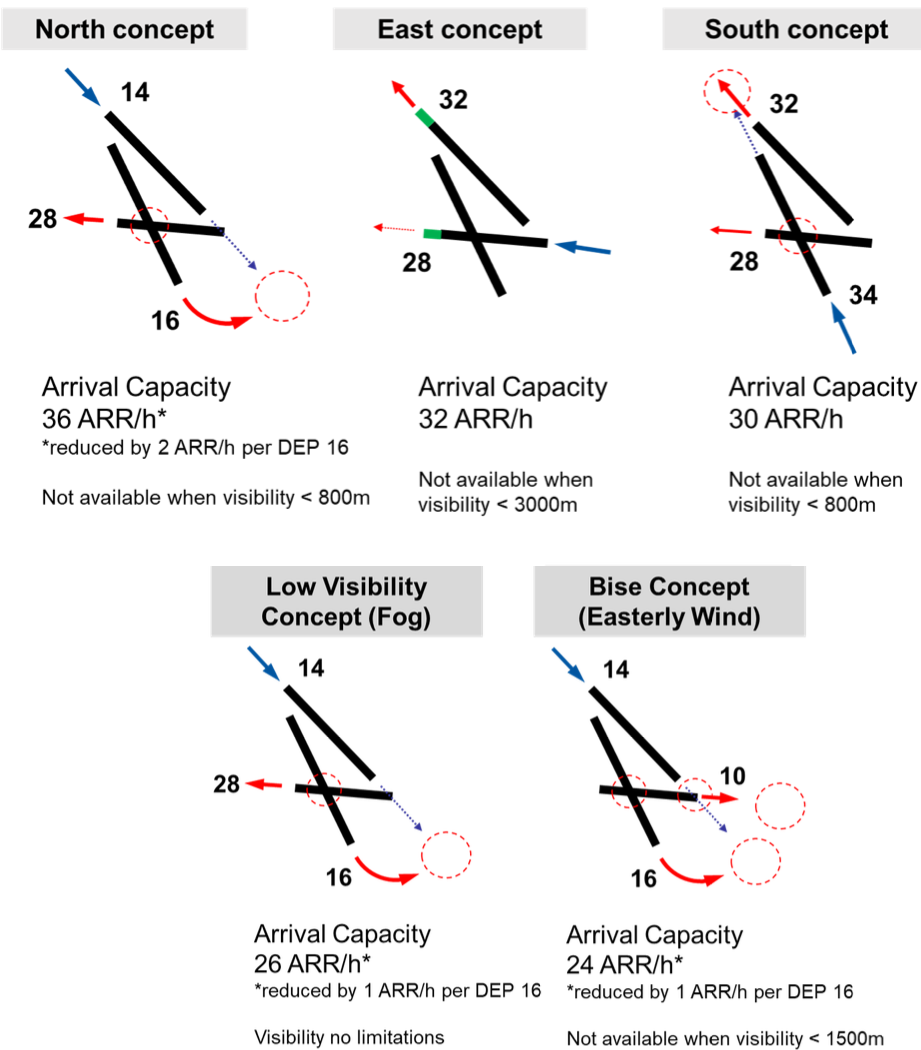
\includegraphics[width=9cm]{Images/Airport Concepts.png}
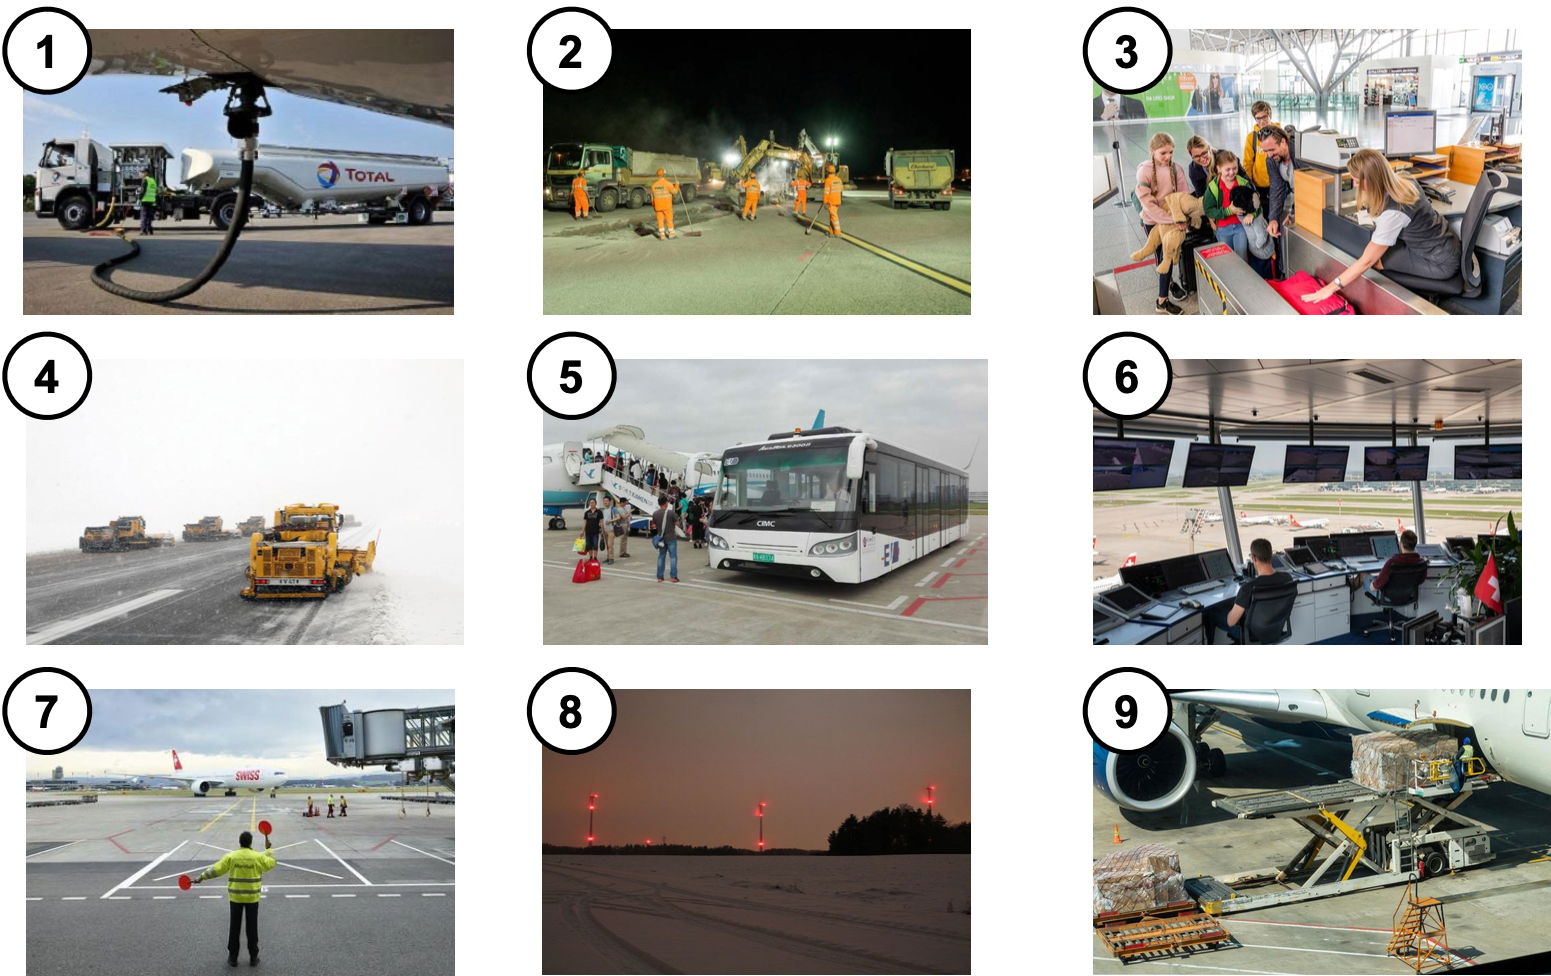
\includegraphics[width=9cm]{Images/Designations.png}
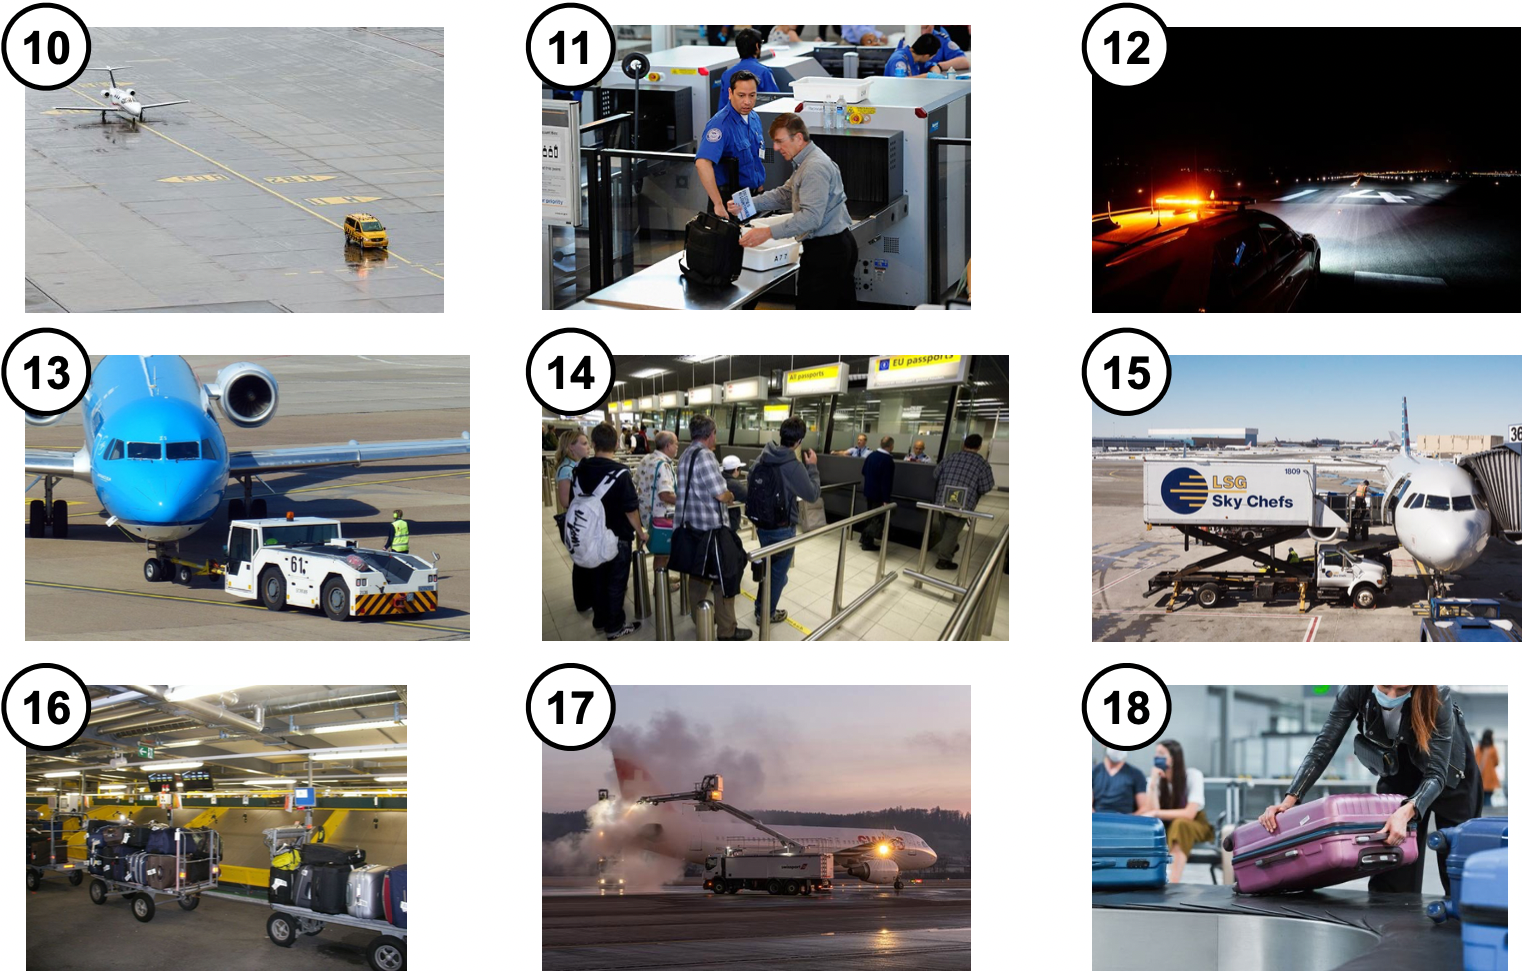
\includegraphics[width=9cm]{Images/Designations2.png}
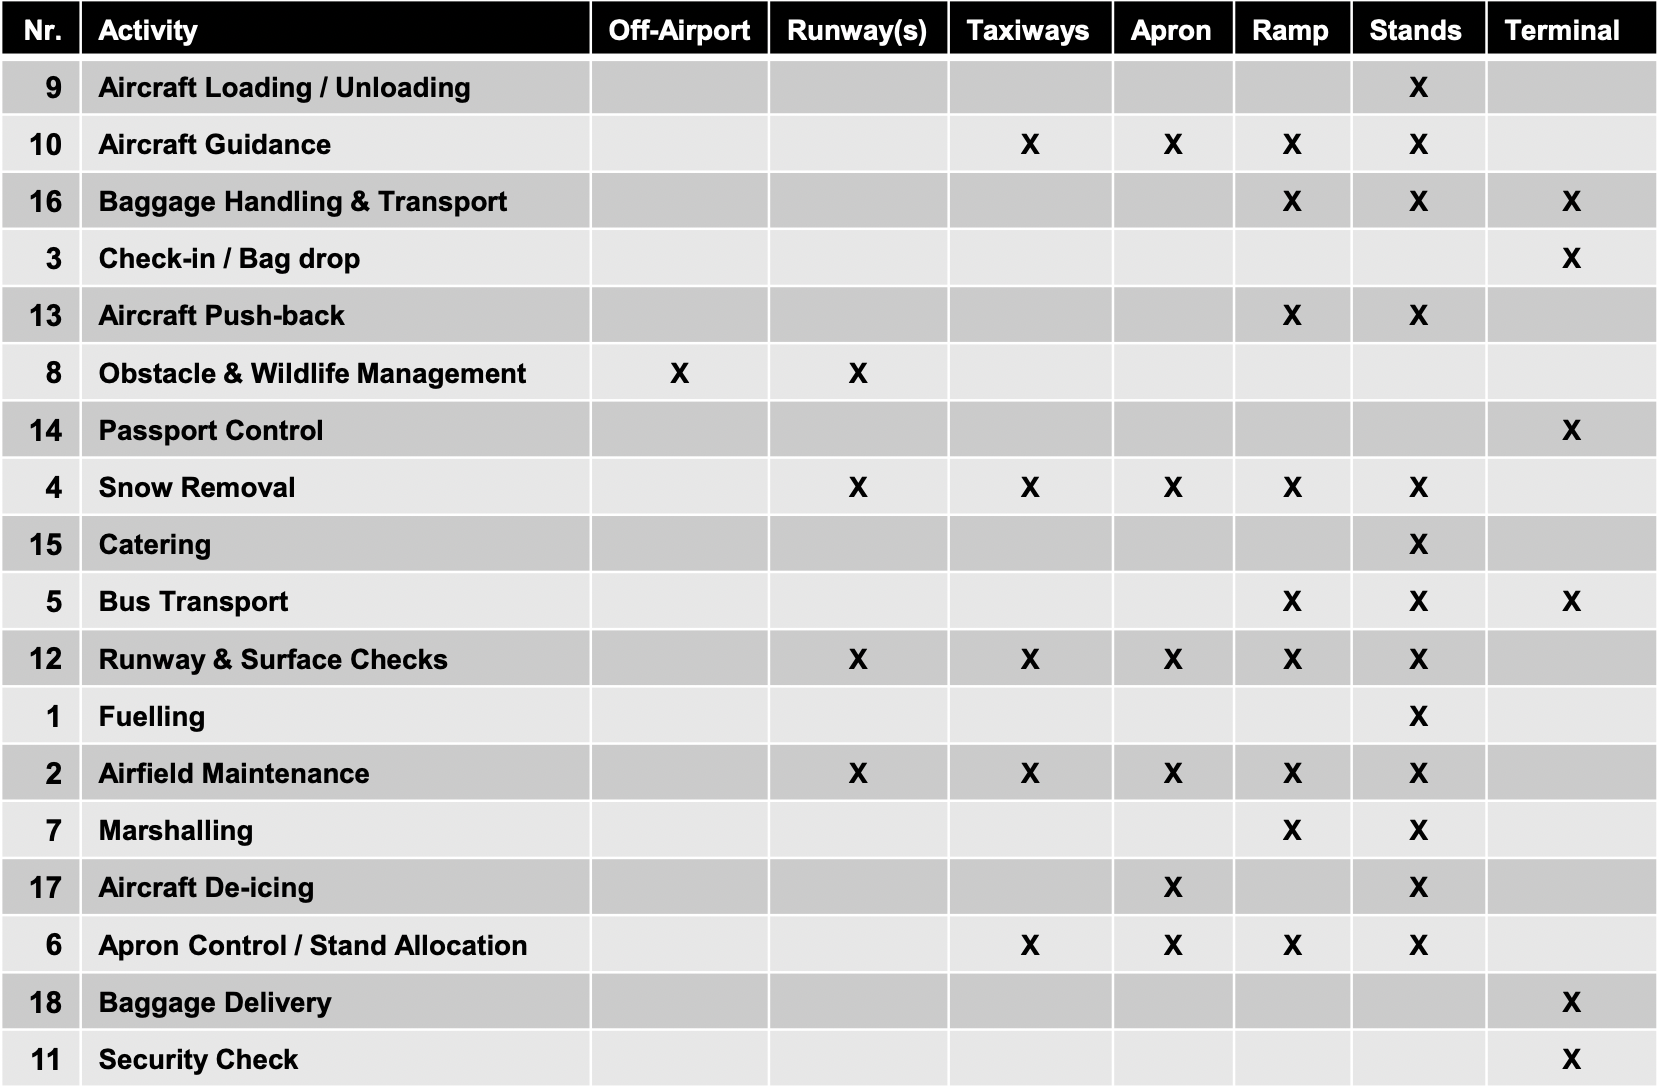
\includegraphics[width=10cm]{Images/Lists_of_Designations.png}
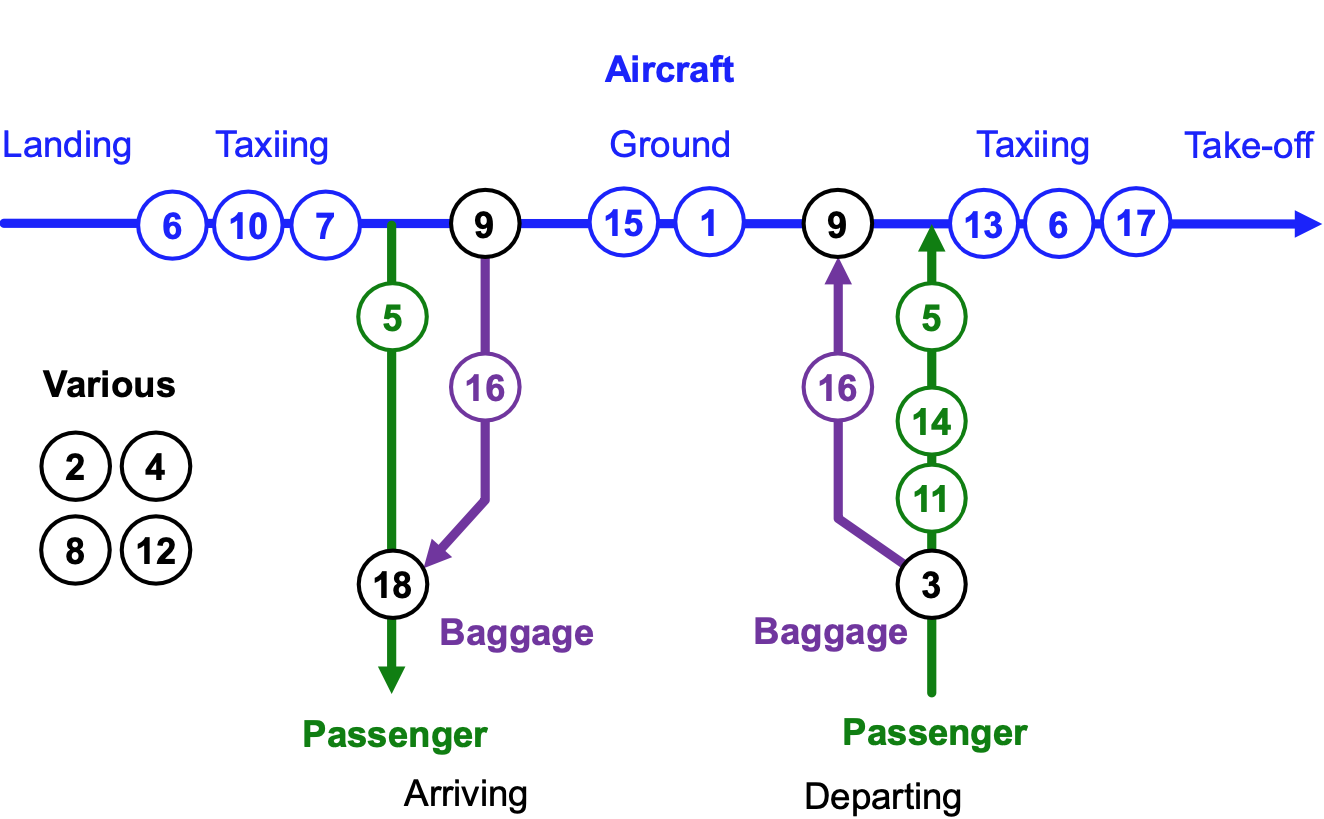
\includegraphics[width=9cm]{Images/Localisation_of_Designations.png}
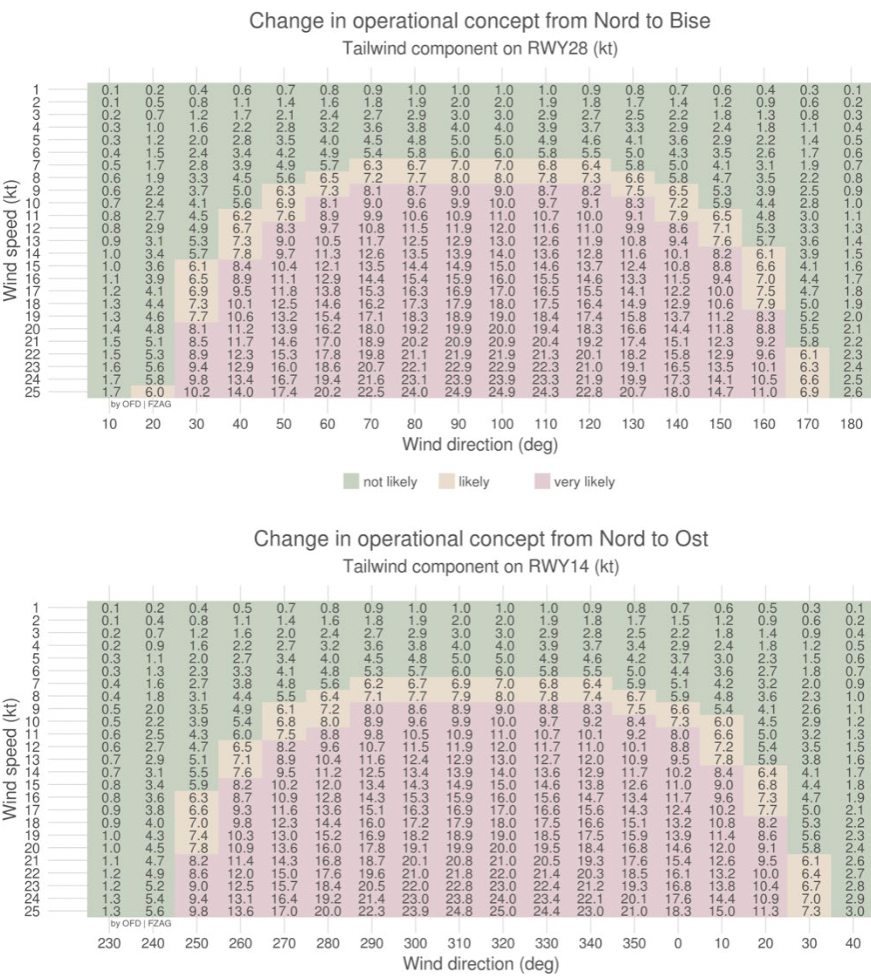
\includegraphics[width=15cm]{Images/Tailwind.png}
\end{center}
\newpage
\section{Air Freight \& Aviation Security}
\underline{\textbf{Air Cargo}} \\ 
\underline{Pre-Covid Numbers (per day)}
\begin{itemize}
    \item 18.6 Billion USD in value Cargo
    \item 29 Million parcells (659 Million on singles day)
    \item 140'000 t Cargo, 898 Million Letters 
    \item 200 race horses 
    \item 1.1 Million Smart Phones 
    \item 80'000 Flowers 
\end{itemize}
\underline{\textbf{Legal and Operational Issues - Part 1}}
\begin{itemize}
    \item Warsaw Convention + The Hague Protocol + Montreal Protocol - in CHF since 1998
    \item Conditions/Contract printed on the back of every Airway Bill (AWB)
    \item Regulates liabilities of the airline, rights of the shipper 
    \item Valid for all air transportation (regular and/or charter)
    \item Most common maximal liabilites for loss or damage 19 SDR per kg gross weight, i.e. approx. 25CHF/kg (Montreal)
    \item SR 748.411 regulates domestic air freight (between ZRH, GVA, BSL, BRN, LUG)
    \item Most countries have their own domestic transport regulations (on top of Warsaw Convention)
    \item IATA achieved standardization of transport conditions, tariffs, documentation + simpflification of transport invoicing
    \item Association IG Cargo: Lobbying, communication + PR, tackling air freight challenges by projects in industry, Exchange of information (cargo forums, presentations)
\end{itemize}
\underline{\textbf{Transport Modes and Documentation}}
\begin{itemize}
    \item Special Freigher Aviation: payload 250t 
    \item Widebody Aircraft: For B747 payload up to 140t 
    \item Narrowboday Aircraft: B737F up to 25t 
    \item Inside: Roller beds for loading/unloading 
    \item Passenger Aircraft: Cargo 50\% fo worldwide transport. However limited in size and weight 
    \item Passenger Aircraft: Loose belly load 
    \item Capacities:
    \begin{itemize}
        \item B777-300 (longhaul): 24t
        \item A380-800 (longhaul): 22t 
        \item A340-300 (longhaul): 20t
        \item A330-300 (long/medium): 18t 
        \item A320-214 (shorthaul): 3t 
        \item AVRO RJ100 (shorthaul): 0.5t
    \end{itemize}
    \item Preighter (Passenger A/C as Freigher): Flexibility 
    \item Transport Devices (Airfreight is loaded either
    loose, on pallets, in containers or in special containers (e.g., refrigerated) into the aircraft)
    \begin{itemize}
        \item Containers
        \item Pallets
    \end{itemize}
    \item Airway Bill (currently printed, should become avail. on the internet) Functions 
    \begin{itemize}
        \item contract of carriage
        \item acknowledgment of receipt
        \item special handling instructions
        \item freight bill 
        \item insurance certificate
        \item customs clearance document
        \item delivery confirmation
    \end{itemize}
\end{itemize}
\underline{\textbf{Infrastructure at Airports}}
\begin{itemize}
    \item Storage and Handling in Air
    \begin{itemize}
        \item Vault for valuables 
        \item Security screenign device 
        \item Animal Cage 
        \item Cool storage 
        \item Radioactive Material 
        \item Express-Channels 
        \item Loading areas 
    \end{itemize}
    \item Cargo Terminal 
    \item Transport to/from A/C 
    \item Loading and unloading of A/C 
\end{itemize}
\underline{\textbf{Goods typically transported by Air}}
\begin{itemize}
    \item Valuables 
    \item Sensitive Materials (Medicine, Laboratory/Research Equipment, Electronics)
    \item Urgent Shipments (Animals, Human Organs, Important Paperwork)
    \item Perishables (Fruits, Flowers, Meat, Food in General)
\end{itemize}
\underline{\textbf{Air Cargo Market Structure}}
\begin{itemize}
    \item Traditional Air Cargo: Combined logistic chains provided by independent airlines, truckers, forwarders and warehouse handlers (numerous service providers, coordinated by freight forwarders on behalf of shipper/seller or buyer/importer)
    \item Integrators: All transports and services provided by one single company
\end{itemize}
\underline{\textbf{Economic Value - Part 2}}
\begin{itemize}
    \item Stakholders 
    \begin{itemize}
        \item Supply Chain: Truckers, Ground Handlers, Security, Airport, Customs, Airline, Consignee, Shipper, Forwarder 
        \item Regulated by: International standards and norms (ICAO, ECAC, IATA), Security Regulations (ICAO, ECAC, IATA), National laws and regulations (FOCA), Customs and health regulations (EZW, BWL, BUVAL)
    \end{itemize}
\end{itemize}
\underline{\textbf{Value of global Air cargo}}
\begin{itemize}
    \item Trade by value: 35\% Air Cargo (6 Trillion per year)
    \item Trade by volume: 1\% Air Cargo 
    \item Cargo moved: 41\% of passenger A/C with Cargo filled 
    \item Air transport without cargo is not economically viable for combined airlines 
    \item COVID: Pre COVID = 94\% A/C used vs COVID = 59\%, rest of Aircraft in service (Total 34250 A/C)
\end{itemize}
\underline{\textbf{Key Figures Air Cargo Switzerland}}
\begin{itemize}
    \item Export: Value Share Swiss exports = 80\% and via swiss airports = 51\% 
    \item Import: Value Share via Swiss Airports = 35\% 
    \item Weight \% = 1\% 
    \item Value per kg export = 1'413
    \item Air Cargo Jobs CH = 25'000
    \item Indirect Air Cargo Jobs = 163'000
    \item Air Cargo: 40\% Metals, 32\% Chemicals and div. Plastics, 21\% Machinery and equip. electricals and watches, 6\% manufactured and 1\% others 
    \item Main destinations: USA (35.1\%), China (12.6\%), Japan (5.9\%), Singapore (4.6\%), Hongkong (3.9\%)... 
\end{itemize}
\underline{\textbf{Challenges}}
\begin{center}
    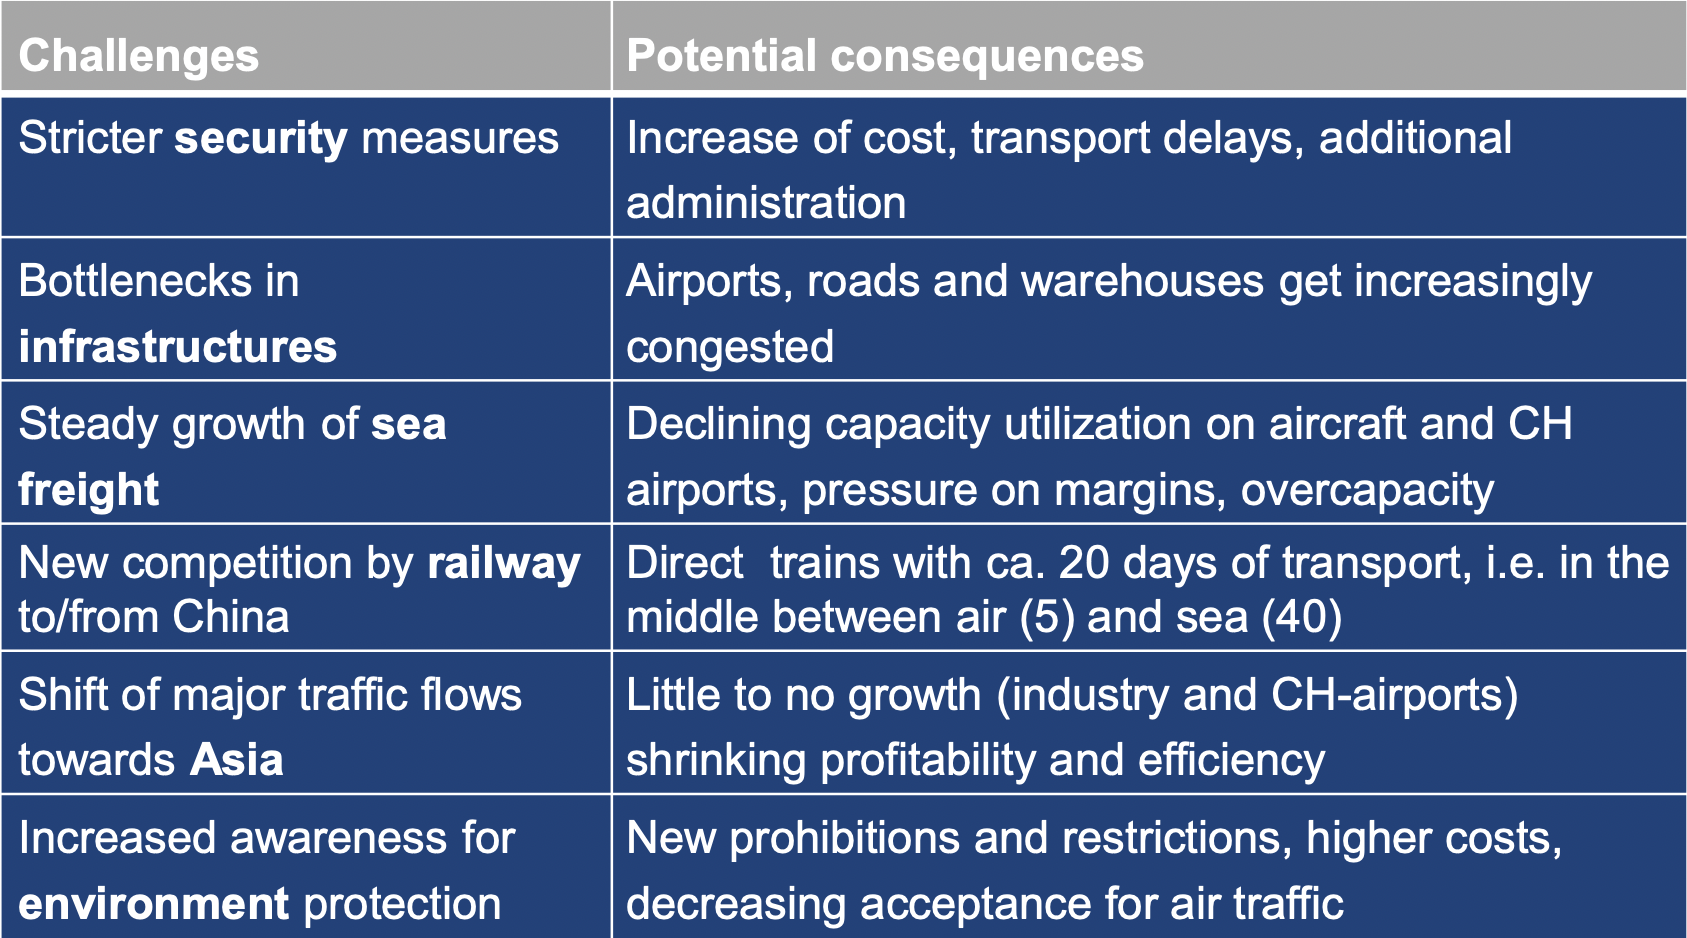
\includegraphics[width=9cm]{Images/Challenges_1.png}
    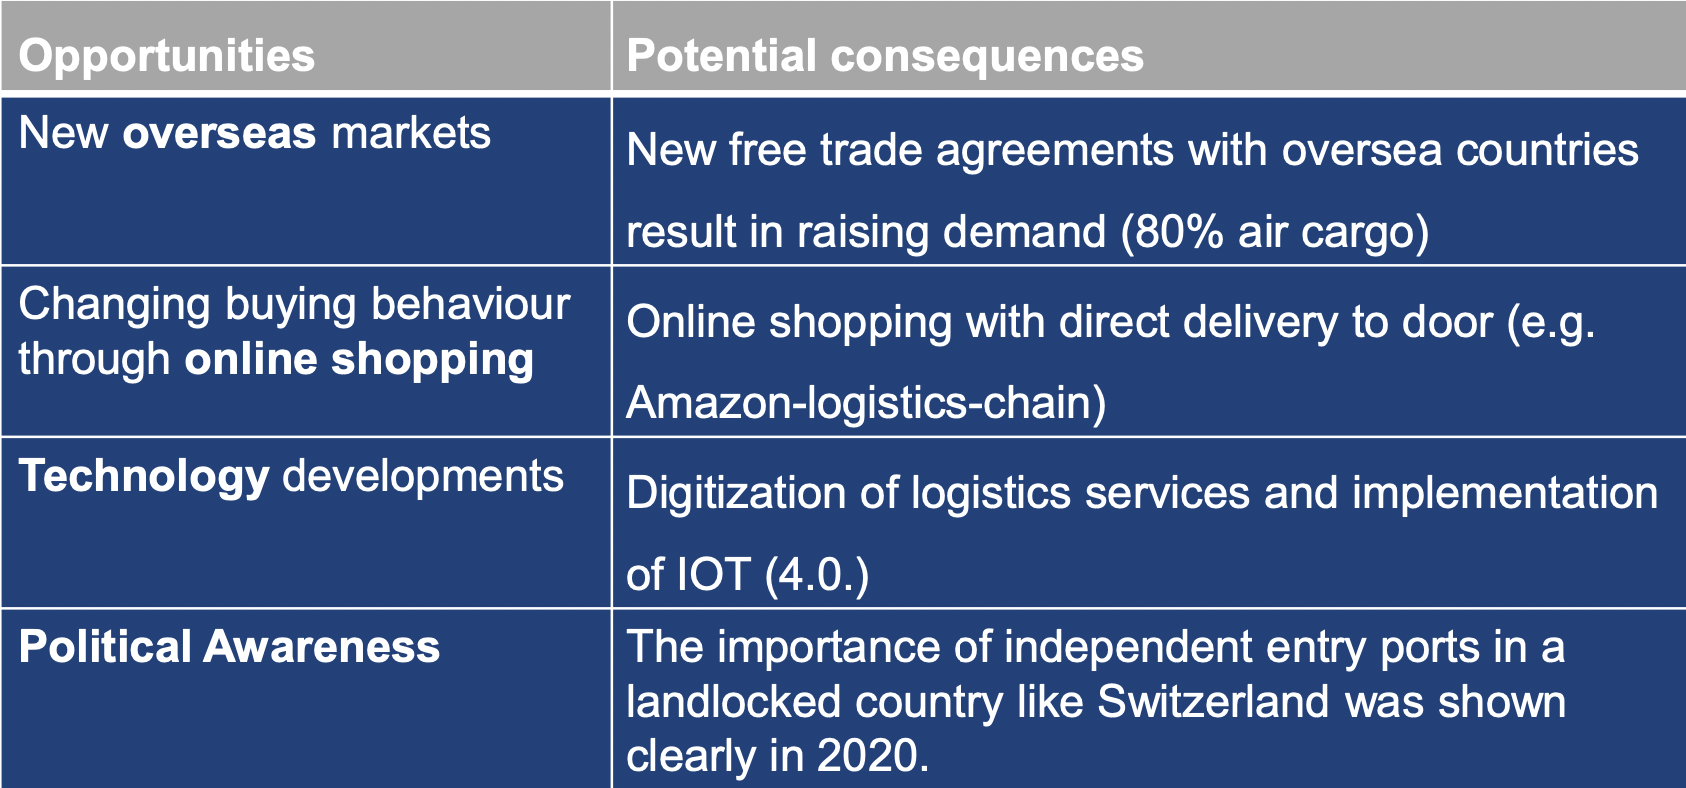
\includegraphics[width=9cm]{Images/Challenges_2.png}
\end{center}
\underline{\textbf{The ideal Swiss air cargo movement}}
\begin{itemize}
    \item Switzerland does not need Mega Cargo Hubs with unlimited space, but needs to focus on it traditional strengths in innovation, quality, reliabiliy and precision. These are the main factors
    \begin{enumerate}
        \item Adequate Infrastructure
        \item Sufficien air transport capacity 
        \item Competitive cost structures 
        \item Lean but clear regulations 
        \item Effective security measures
        \item Electronic data exchange 
        \item Opennness for new developments 
    \end{enumerate}
\end{itemize}
\underline{\textbf{Future}} \\ \\
World air cargo traffic is still expected to growth annualy 4\% over the next 20 years. E-commerce is expected to double every four years
\begin{itemize}
    \item Green/Sustainable 
    \item Being prepared 
    \item Business travel
    \item Narrow-body long-haul 
    \item Cargo vs Pax Airlines 
    \item Open Borders 
    \item Reform 
\end{itemize}
\underline{\textbf{Environmental Aspects - Part 3}}
\begin{itemize}
    \item Responsibility of logistics and transport 
    \begin{itemize}
        \item Logistics \& Transport has second largest share of CO2 emissions (24\%)
        \item In 2050, the European Energy Agency (IEA) expects that global logistics will have the largest share with up to 40\% (globalisation effect)
    \end{itemize}
    \item Huge differences in CO2 emmisions (Example Hamburg-Istanbul) - weight 500kg + no cooling 
    \begin{itemize}
        \item A321: 706 kg 
        \item Boeing 777F (freighter): 435 kg 
        \item Truck (40t): 503 kg 
        \item Container ship: 10 kg 
        \item Rail: 7kg  
    \end{itemize}
    \item Emission values of day to day products 
    \begin{itemize}
        \item CO2 output significantly higher for Air transport compared to ship 
    \end{itemize}
    \item Calculations and Compensation 
    \begin{itemize}
        \item At Zurich Airport one ton air cargo produces an average of 11 kg CO2
        \begin{itemize}
            \item 95\% by flight movements
            \item 3\% from truck transports
            \item 2\% from the airport (handling, heating, electricity, etc.)
        \end{itemize}
    \end{itemize}
    \item Conclusion and recommendation
    \begin{itemize}
        \item with the choice of the right mode of transport the emission output can be reduced
        \item Railway transport has the lowest and air cargo the highest output of CO2 per kg, however, the impact of air cargo on the global emission effects is low due to the low volumes carried by air
        \item Companies must set clear reduction goals and implement measures. They must establish clear policies when choosing their transports
        \begin{itemize}
            \item Avoid
            \item Optimise 
            \item Measure 
            \item Compensate 
        \end{itemize}
        \item Awareness in the society must be raised that not only passenger trips are generating greenhouse gases but also transport and logistics services
    \end{itemize}
\end{itemize}
\underline{\textbf{Aviation Security}}
\begin{itemize}
    \item Safety 
    \begin{itemize}
        \item Safety: Deals with preventive measures against the occurrence of events that have their origin in unintentional human and / or technical inadequacies.
        But also deals with comprehensive safety for the life and health of employees at their workplace (= occupational safety).
    \end{itemize}
    \item Security 
    \begin{itemize}
        \item Addresses preventive measures against the occurrence of events that are committed by people with willful intent against companies or organizations, as well as the limitation or control of such incidents and the damage resulting
        from them.
    \end{itemize}
    \item Most efficient security: Control the bad and leave the good
\end{itemize}
\underline{Threats}
\begin{itemize}
    \item Risk Analysis (targets of attacks are): 
    \begin{itemize}
        \item Passangers/employees 
        \item Airport Infrastructure
        \item Airplanes 
        \item Hijacking 
        \item Sabotage 
        \item Other airplanes as weapons 
    \end{itemize}
    \item Why civil aviation is an attractive target
    \begin{enumerate}
        \item Global reach, even if local 
        \item Rapid transmission of information, increasing audience
        \item Depriciate the embodiment of state power that airlines and airports symbolise 
        \item Powerful economic consequences beyond civil aviation 
        \item High lethal potential, and high probability of effecting people from multiple countries at once 
        \item Impede interconnectivity, disrupting global air transport 
        \item Instantly making powerful statements to world leaders  
    \end{enumerate}
    \item Types of Security Checks 
    \begin{itemize}
        \item Security Checks of passengers and baggage 
        \item ... staff and goods 
        \item Security measures for aircraft 
        \item ... checks of air freight and air mail 
        \end{itemize}
    \item Security Equipment 
\end{itemize}
\begin{center}
    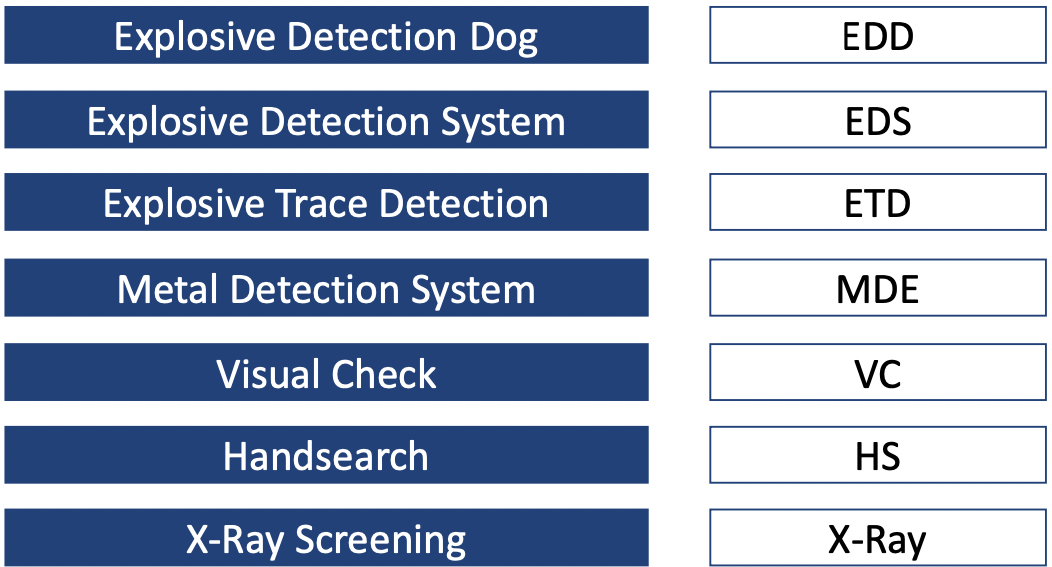
\includegraphics[width=8cm]{Images/Security Equipment.png}
\end{center}
\begin{itemize}
    \item Objects to be found
    \begin{itemize}
        \item Dangerous goods: Are not forbidden, but can be used to threaten or injure people or can cause fire and explosions
        \item Prohibited items: are forbidden under the weapons act 
    \end{itemize}
    \item Number one weapon, the Unpredicitability of passengers and luggage 
    \begin{itemize}
        \item Selected at random, and choice is not made by staff 
    \end{itemize}
    \item Legal requirements 
    \begin{itemize}
        \item FOCA: Supervisory of CH through NASP 
        \item NASP: The NASP (National Aviation Security Program) defines the standards and their implementation. Framework instructions to the participating entities are defined in it.
    \end{itemize}
    \item Future 
    \begin{itemize}
        \item Human Security Radar 
        \item Categorisation of Passengers 
        \item Drone Defence Systems 
    \end{itemize}
    \item Future Demands 
    \begin{itemize}
        \item Intelligence: Passenger differentiation based on risk and trust 
        \item Innovation: New control technology and processes
        \item Service: Different understanding of work in the aviation security sector
    \end{itemize}
    \item Current Weaknesses of today's security systems 
    \begin{itemize}
        \item Too tech-heavy 
        \item Overregulated 
        \item Pseudo Security 
    \end{itemize}
    \item Solutions 
    \begin{itemize}
        \item Raising employee awareness 
        \item Organisation with high reliability
    \end{itemize}
\end{itemize}
\end{multicols*}
\end{document}

